\documentclass[a4paper,12pt
,draft
% ,final
]{article}%

\pdfcompresslevel=0
\pdfobjcompresslevel=0

\usepackage{xr-hyper}
\usepackage[pagebackref, colorlinks, citecolor=PineGreen, linkcolor=PineGreen]{hyperref}
\hypersetup{
  final,
  pdftitle={On the homotopy theory of equivariant colored operads},
  pdfauthor={Bonventre, P. and Pereira, L. A.},
  linktoc=page
}

\externaldocument[TAS-]{TameAndSquare} % cite using names from other half


% ---- Commands on draft --------

\usepackage[dvipsnames]{xcolor}% adds colors
\usepackage{ifdraft}
\ifdraft{
  \color[RGB]{63,63,63}
  \pagecolor[RGB]{220,220,204}
  \usepackage[notref]{showkeys}
  \usepackage[margin=1in]{geometry}
  \usepackage{todonotes}
}
{
  \usepackage[notref]{showkeys}
  \usepackage[margin=1in]{geometry}
  \usepackage[disable]{todonotes}
  \usepackage[fontsize=12pt]{scrextend}
}

\usepackage{amsmath, amsthm}% {amsfonts, amssymb}


% ------ New Characters --------------------------------------

\usepackage[latin1]{inputenc}%
\usepackage{MnSymbol}
\DeclareMathAlphabet\mathbb{U}{msb}{m}{n}
%\usepackage{stmaryrd}
%\usepackage{upgreek}
\usepackage{mathrsfs}
% \usepackage[T1]{fontenc}
% \usepackage[english]{babel}
% \usepackage{fouriernc}
% \DeclareMathAlphabet{\mathscr}{U}{mathrsfs}{m}{n}`

\usepackage[normalem]{ulem}%
\usepackage{dsfont}%
\usepackage{bbm}%



%----- Enumerate ---------------------------------------------
% \usepackage{paralist} % for inparaenum
% \usepackage{enumerate}%
\usepackage[inline,shortlabels]{enumitem}% % can use \begin{enumerate*} for inparaenum


% ---------- Page Typesetting ----------
\usepackage[final]{microtype}
\usepackage{relsize}


%-------- Tikz ---------------------------

\usepackage{tikz}%
\usetikzlibrary{matrix,arrows,decorations.pathmorphing,
cd,patterns,calc}
\tikzset{%
  treenode/.style = {shape=rectangle, rounded corners,%
                     draw, align=center,%
                     top color=white, bottom color=blue!20},%
  root/.style     = {treenode, font=\Large, bottom color=red!30},%
  env/.style      = {treenode, font=\ttfamily\normalsize},%
  dummy/.style    = {circle,draw,inner sep=0pt,minimum size=2mm}%
}%

\usetikzlibrary[decorations.pathreplacing]


% ----- Labels Changed? --------

\makeatletter

\def\@testdef #1#2#3{%
  \def\reserved@a{#3}\expandafter \ifx \csname #1@#2\endcsname
  \reserved@a  \else
  \typeout{^^Jlabel #2 changed:^^J%
    \meaning\reserved@a^^J%
    \expandafter\meaning\csname #1@#2\endcsname^^J}%
  \@tempswatrue \fi}

\makeatother


%%%%%%%%%%%%%%%%%%%%%%%%% INTERNAL REFERENCES %%%%%%%%%%%%%%%%%%%%%%%%%%%%%%%%%%%

\numberwithin{equation}{section} 
\numberwithin{figure}{section}

\usepackage{mathtools}
\mathtoolsset{showonlyrefs,showmanualtags} % Only number equations which are referenced with eqref


% ------- New Theorems/ Definition/ Names-----------------------

 % \theoremstyle{plain} % bold name, italic text
\newtheorem{theorem}[equation]{Theorem}%
\newtheorem*{theorem*}{Theorem}%
\newtheorem{lemma}[equation]{Lemma}%
\newtheorem{proposition}[equation]{Proposition}%
\newtheorem{corollary}[equation]{Corollary}%
\newtheorem{conjecture}[equation]{Conjecture}%
\newtheorem*{conjecture*}{Conjecture}%
\newtheorem{claim}[equation]{Claim}%

%%%%%% Fancy Numbering for Theorems
\newtheorem{innercustomgeneric}{\customgenericname}
\providecommand{\customgenericname}{}
\newcommand{\newcustomtheorem}[2]{%
  \newenvironment{#1}[1]
  {%
   \renewcommand\customgenericname{#2}%
   \renewcommand\theinnercustomgeneric{##1}%
   \innercustomgeneric
  }
  {\endinnercustomgeneric}
}

\newcustomtheorem{customthm}{Theorem}
\newcustomtheorem{customcor}{Corollary}
%%%%%%%%%%%%%

\theoremstyle{definition} % bold name, plain text
\newtheorem{definition}[equation]{Definition}%
\newtheorem*{definition*}{Definition}%
\newtheorem{example}[equation]{Example}%
\newtheorem{remark}[equation]{Remark}%
\newtheorem{notation}[equation]{Notation}%
\newtheorem{convention}[equation]{Convention}%
\newtheorem{assumption}[equation]{Assumption}%
\newtheorem{exercise}{Exercise}%


% %%%%%%%%%%%%%%%%%%%%%%%%%%%%%%%%%%%%%%%%%%%%%%%%%%%%%%%%%%%%%%%%%%%%%%%%%%%%%%%%
% ------------------------------ COMMANDS ------------------------------

% ---------- macros

\newcommand{\set}[1]{\left\{#1\right\}}%
\newcommand{\sets}[2]{\left\{ #1 \;|\; #2\right\}}%
\newcommand{\longto}{\longrightarrow}%
\newcommand{\into}{\hookrightarrow}%
\newcommand{\onto}{\twoheadrightarrow}%

\usepackage{harpoon}
\newcommand{\vect}[1]{\text{\overrightharp{\ensuremath{#1}}}}


% ---------- operators

\newcommand{\Sym}{\ensuremath{\mathsf{Sym}}}%
\newcommand{\Fin}{\mathsf{F}}%
\newcommand{\Set}{\ensuremath{\mathsf{Set}}}
\newcommand{\Top}{\ensuremath{\mathsf{Top}}}
\newcommand{\sSet}{\ensuremath{\mathsf{sSet}}}%
\newcommand{\Cat}{\mathsf{Cat}}
\newcommand{\sCat}{\mathsf{sCat}}
\newcommand{\Op}{\mathsf{Op}}%
\newcommand{\sOp}{\ensuremath{\mathsf{sOp}}}%
\newcommand{\fgt}{\ensuremath{\mathsf{fgt}}}%
\newcommand{\dSet}{\mathsf{dSet}}
\newcommand{\Fun}{\mathsf{Fun}}
\newcommand{\Fib}{\mathsf{Fib}}
\newcommand{\Alg}{\mathsf{Alg}}
\newcommand{\Kl}{\mathsf{Kl}}



\DeclareMathOperator{\hocmp}{hocmp}%
\DeclareMathOperator{\cmp}{cmp}%
\DeclareMathOperator{\hofiber}{hofiber}%
\DeclareMathOperator{\fiber}{fiber}%
\DeclareMathOperator{\hocofiber}{hocof}%
\DeclareMathOperator{\hocof}{hocof}%
\DeclareMathOperator{\holim}{holim}%
\DeclareMathOperator{\hocolim}{hocolim}%
\DeclareMathOperator{\colim}{colim}%
\DeclareMathOperator{\Lan}{Lan}%
\DeclareMathOperator{\Ran}{Ran}%
\DeclareMathOperator{\Map}{Map}%
\DeclareMathOperator{\Id}{Id}%
\DeclareMathOperator{\mlf}{mlf}%
\DeclareMathOperator{\Hom}{Hom}%
\DeclareMathOperator{\Ho}{Ho}
\DeclareMathOperator{\Aut}{Aut}%
\DeclareMathOperator{\Stab}{Stab}
\DeclareMathOperator{\Iso}{Iso}
\DeclareMathOperator{\Ob}{Ob}

% ---------- shortcuts

\newcommand{\F}{\ensuremath{\mathcal F}}
\newcommand{\V}{\ensuremath{\mathcal V}}
\newcommand{\Q}{\ensuremath{\mathcal Q}}
\renewcommand{\O}{\ensuremath{\mathcal O}}
\renewcommand{\P}{\ensuremath{\mathcal P}}
\newcommand{\C}{\ensuremath{\mathcal C}}
\newcommand{\A}{\ensuremath{\mathcal A}}
\newcommand{\G}{\ensuremath{\mathcal G}}

\newcommand{\del}{\partial}%

\newcommand{\ki}{\chi}
\newcommand{\ksi}{\xi}
\newcommand{\Ksi}{\Xi}

\newcommand{\lltimes}{\underline{\ltimes}}

% detecting $\V$-categories:

\newcommand{\I}{\mathbb I}
\newcommand{\J}{\mathbb J}
\newcommand{\1}{\ensuremath{\mathbbm 1}}%{\ensuremath{\mathbb{id}}} %\eta

% lazy shortcuts

\newcommand{\SC}{\Sigma_{\mathfrak C}}
\newcommand{\OC}{\Omega_{\mathfrak C}}
\newcommand{\UV}{\underline{\mathcal V}}
\newcommand{\UC}{\underline{\mathfrak C}}










% %%%%%%%%%%%%%%%%%%%%%%%%%%%%%%%%%%%%%%%%%%%%%%%%%%%%%%%%%%%%%%%%%%%%%%%%%%%%%%%%%%%%%%%%%%%%%%%%%%%%
% ------------------------------ MAIN BODY ------------------------------

% ---- Title --------

\title{Fibered adjunctions and the monad for equivariant colored operads}

\author{Peter Bonventre, Lu\'is A. Pereira}%

\date{\today}


% ---- Document body --------

\begin{document}

\maketitle

\begin{abstract}
	We build model structures 
	on the category of equivariant simplicial operads
	with weak equivalences determined by families of subgroups,
	both in the context of operads with a fixed set of colors and in the context of all colored operads.
	In particular, specifying to the family of graph subgroups 
	(or, more generally, the indexing systems of Blumberg-Hill),
	this yields model structures on the category of equivariant simplicial operads
	whose weak equivalences are determined by norm map data.
\end{abstract}



\tableofcontents





\section{Intro}

Stuff
\newpage


\section{Preliminaries}\label{PRE SEC}


Much as in the non-equivariant case, 
our approach to building the model structures
in Theorem \ref{THMIII} on the category
$\mathsf{Op}^G_{\bullet}(\V)$
of equivariant operads on all sets of colors
will be to first build the model structures in Theorem \ref{THMI}
on the subcategories
$\mathsf{Op}^G_{\mathfrak{C}}(\V)$
with a fixed $G$-set of colors $\mathfrak{C}$.

However, the equivariant setting presents some technical challenges that will require us to repackage the non-equivariant narrative of
\cite{CM13b},\cite{Cav} somewhat.

To see why, recall that \cite{CM13b},\cite{Cav}
follow a ``work color by color and then assemble'' strategy.
More precisely, first the model structures on fixed color operads 
$\mathsf{Op}_{\mathfrak{C}}(\V)$
are built by identifying these as algebras over a monad
$\mathbb{F}_{\mathfrak{C}}$
on the category $\mathsf{Sym}_{\mathfrak{C}}(\V)$
of fixed color symmetric sequences,
with maps of operads that do not fix colors
only appearing afterwards when assembling the model structure on the full category $\mathsf{Op}_{\bullet}(\V)$.

However, when working equivariantly, 
while the maps in the fixed $G$-set of objects categories 
$\mathsf{Op}^G_{\mathfrak{C}}(\V)$ do fix colors, 
the $G$-action on \emph{objects}
$\O \in \mathsf{Op}^G_{\mathfrak{C}}(\V)$
involves maps of operads $\O \xrightarrow{g} \O$
that need not fix colors (unless $\mathfrak{C}$ is a trivial $G$-set).
In other words, when discussing equivariant operads even the fixed color categories 
$\mathsf{Op}^G_{\mathfrak{C}}(\V)$
requires color change data.
Due to this issue, 
our approach will be that the transition from the non-equivariant to the equivariant case is easier to describe 
if we regard the global framework,
where we consider all colors at once, as the primary framework
and then restrict to color fixed operads only when needed.

More explicitly, the basis of our approach is to combine the 
fixed color symmetric sequence categories
$\mathsf{Sym}_{\mathfrak{C}}(\V)$ for all color sets 
$\mathfrak{C} \in \mathsf{Set}$
and change of color data between them into a single category
$\mathsf{Sym}_{\bullet}(\V)$.
There is then a Grothendieck fibration
$\mathsf{Sym}_{\bullet}(\V) \to \mathsf{Set}$
which records the underlying set of colors,
and whose fiber over $\mathfrak{C}$ is 
$\mathsf{Sym}_{\mathfrak{C}}(\V)$.
Similarly, the monads $\mathbb{F}_{\mathfrak{C}}$ (and change of color data between them) 
assemble into a single monad $\mathbb{F}$
on $\mathsf{Sym}_{\bullet}(\V)$
which is suitably compatible with 
the Grothendieck fibration 
$\mathsf{Sym}_{\bullet}(\V) \to \mathsf{Set}$,
and by considering (a subcategory of) algebras over $\mathbb{F}$
one obtains the category $\mathsf{Op}_{\bullet}(\V)$
of colored operads for all colors.
These fit together as on the left below.
\begin{equation}\label{FIBADJMON EQ}
\begin{tikzcd}[row sep = small, column sep = tiny]
\Sym_\bullet(\V) \arrow[rr, "\mathbb F"] \arrow[dr]
&&
\Op_\bullet(\V) \arrow[dl]
&&& % ----------
\Sym^G_\bullet(\V) \arrow[rr, "\mathbb F^G"] \arrow[dr]
&&
\Op^G_\bullet(\V) \arrow[dl]
\\
&
\mathsf{Set}
&
&&& % ----------
&
\mathsf{Set}^G
\end{tikzcd}
\end{equation}
Within this global framework, passing to the equivariant case is simply a matter of applying $G$-objects throughout as on the right above, 
so that one has a Grothendieck fibration
$\mathsf{Sym}_{\bullet}^G \to \mathsf{Set}^G$
with a compatible monad $\mathbb{F}^G$
from which one obtains the category 
$\mathsf{Op}_{\bullet}(\V)$
of $G$-equivariant colored operads for all colors. 


The plan for this preliminary section is then as follows.
%
\S \ref{GROTFIB SEC} recalls the notion of Grothendieck fibration and
introduces some related constructions that are used throughout.
%
\S \ref{FIBCAT_SEC} discusses how the usual notions of adjunction and monad interact with Grothentieck fibrations,
allowing us to regard the monads
(and associated adjunctions)
in \eqref{FIBADJMON EQ}
as being suitably fibered over $\mathsf{Set}$ and $\mathsf{Set}^G$.
%
\S \ref{EQCOSYMSEQ SEC} then applies the abstract theory in 
\S \ref{GROTFIB SEC},\ref{FIBCAT_SEC}
to discuss the global categories
$\mathsf{Sym}_{\bullet}(\V)$,
$\mathsf{Sym}^G_{\bullet}(\V)$
of symmetric sequences, 
with most of the work being devoted to providing 
explicit descriptions of the equivariant fibers
$\mathsf{Sym}^G_{\mathfrak{C}}(\V)$
for $\mathfrak{C} \in \mathsf{Set}^G$
and of the representable functors in these fibers.
%
Lastly, in \S \ref{EQCOSYMOP SEC}, 
we describe the fibered monad $\mathbb F$ (Equation \eqref{FREEOP_EQ}, elaborated in Appendix \ref{MONAD_APDX}),
and determine the fibers of the equivariant monad $\mathbb F^G$ (Equation \eqref{FGC_EQ}).


As a side note, we observe that our discussion of fibered category theory will also help streamline our work in the sequel.
Therein, we will need to establish a Quillen equivalence
$\tau \colon \mathsf{PreOp}^G \rightleftarrows \mathsf{sOp}^G\colon N$
between the category of (simplicial) preoperads and
the category of simplicial operads.
In that work, the claim that the adjunction is Quillen 
will be greatly simplified by noting that in both categories 
the generating (trivial) cofibrations
can be described using a ``fibered simplicial cotensoring''.





\subsection{Grothendieck fibrations}\label{GROTFIB SEC}


Recall that a functor 
$\pi \colon \mathcal{C} \to \mathcal{B}$
is called a \emph{Grothendieck fibration}
if for all arrows
$\varphi \colon b' \to b$ in $\mathcal{B}$
and $c \in \mathcal{C}$ such that $\pi(c) = b$
there exists a \emph{cartesian arrow}
$\varphi^{\**}c \to c$
lifting $\varphi$,
meaning that for any choice of solid arrows
\begin{equation}\label{CARTARDEF EQ}
\begin{tikzcd}
c'' \ar{rr} \ar[dashed]{rd}[swap]{\exists!} 
&&
c
&%%
b'' \ar{rr} \ar{rd} 
&&
b
\\
& \varphi^{\**} c \ar{ru}
&
&%%
& b'\ar{ru}[swap]{\varphi}
&
\end{tikzcd}
\end{equation}
such that the right diagram commutes and 
$c'' \to c$ lifts $b'' \to b$,
there exists a unique dashed arrow
$c'' \to \varphi^{\**} c$ lifting $b'' \to b'$
and making the left diagram commute.


Moreover, writing $\mathcal{C}_b$ for the fiber over $b \in \mathcal{B}$,
a \emph{cleavage} of $\pi$ is a fixed choice of cartesian arrows
$\varphi^{\**} c \to c$
for each $\varphi \colon b' \to b$ and $c$ with $\pi(c)=b$.


Dually, if $\pi^{op} \colon \mathcal{C}^{op} \to \mathcal{B}^{op}$
is a Grothendieck fibration we 
say that $\pi$ is a \emph{Grothendieck opfibration}.
More explicitly, this means that for any arrow
$\varphi \colon b \to b'$ in $\mathcal{B}$
and $c \in \mathcal{C}$ such that 
$\pi(c) = b$ there exists a 
\emph{cocartesian arrow}
$c \to \varphi_! c$ lifting $\varphi$
and satisfying the dual of the universal property in 
\eqref{CARTARDEF EQ}.
A cleavage of an opfibration is similarly defined as a fixed choice
of cocartesian arrows 
$c \to \varphi_!c$.



\begin{notation}\label{MAPSDEC NOT}
Given any functor of categories
$\pi \colon \mathcal{C} \to \mathcal{B}$,
one has a natural decomposition of mapping sets
\begin{equation}
\mathcal{C}(c',c) = 
\coprod_{f \in \mathcal{B}(\pi(c'),\pi(c))}
 \mathcal{C}_{\varphi}\left(c',c \right)
\end{equation}
where $\mathcal{C}_{\varphi}\left(c',c \right)$ consists of the arrows projecting to $\varphi$.
\end{notation}



\begin{remark}\label{CARTCHAR REM}
Note that, specifying to the case $b'' = b'$ in 
\eqref{CARTARDEF EQ},
one has that when $\pi$ is a Grothendieck fibration the contravariant functors
\begin{equation}\label{FIXPIREP EQ}
\mathcal{C}_{\varphi}(-,c)
\colon
\mathcal{C}_{b'} 
\to
\mathsf{Set}
\end{equation}
are represented by (some choice of) $\varphi^{\**}c$.
Moreover, note that under the representing isomorphism
$\mathcal{C}_{b'}(\varphi^{\**}c,\varphi^{\**}c)
\simeq \mathcal{C}_{\varphi}(\varphi^{\**}c,c)$
the identity
$\varphi^{\**}c \xrightarrow{=} \varphi^{\**}c$
yields the canonical map
$\varphi^{\**}c \to c$ over $\varphi$.
\end{remark}


\begin{remark}\label{COMPSEMI REM}
The universal condition in \eqref{CARTARDEF EQ}
is stronger than the representability of 
\eqref{FIXPIREP EQ}.
More precisely, let us say an arrow 
$\varphi^{\**}c \to c$
is weakly cartesian if it represents \eqref{FIXPIREP EQ},
and that  
$\pi \colon \mathcal{C} \to \mathcal{B}$
is a weak Grothendieck fibration if it admits all weakly cartesian arrows.
Then $\pi$ is in fact a Grothendieck fibration,
i.e. the weakly cartesian arrows 
$\varphi^{\**}c \to c$
satisfy the stronger condition in \eqref{CARTARDEF EQ},
iff the composites of weakly cartesian arrows are again weakly cartesian, 
i.e. if 
for any composable arrows
$b'' \xrightarrow{\psi} b' \xrightarrow{\varphi} b$
and $c$ with $c \in \mathcal{C}_b$ it is
$\psi^{\**} \varphi^{\**} c \simeq 
\left( \varphi \psi \right)^{\**} c$,
where the isomorphism is in $\mathcal{C}_b$.
\end{remark}



\begin{remark}\label{ALSOOPADJ REM}
Using the universal property \eqref{CARTARDEF EQ},
a cleavage of a Grothendieck fibration 
$\pi \colon \mathcal{C} \to \mathcal{B}$
defines functors
$f^{\**} \colon \mathcal{C}_b \to \mathcal{C}_{b'}$
for each arrow $f \colon b' \to b$.

Moreover, 
the claim that $\pi$ is also an opfibration is then equivalent to the existence of left adjoints
\[
	\varphi_! \colon
	\mathcal{C}_{b'}
	\rightleftarrows
	\mathcal{C}_{b}
	\colon \varphi^{\**}
\]
for all arrows $\varphi \colon b' \to b$ in $\mathcal{B}$.
%
We note that the required condition that the functors
$\varphi_! \psi_!$ and
$(\varphi \psi)_!$
are naturally isomorphic (cf. Remark \ref{COMPSEMI REM})
is automatic, 
since these are left adjoints to 
$\psi^{\**} \varphi^{\**} \simeq 
\left( \varphi \psi \right)^{\**}$.
\end{remark}


\begin{remark}\label{FUNISGROTH REM}
Let $\pi \colon \mathcal{C} \to \mathcal{B}$
be a Grothendieck fibration and
$I$ a diagram category.
Then, 
writing $\mathcal{C}^{I}$ for the category of functors 
$I \to \mathcal{C}$ and likewise for $\mathcal{B}^I$,
the functor
$\pi^I \colon \mathcal{C}^I \to \mathcal{B}^I$
is again a Grothendieck fibration, with cartesian arrows in $\mathcal{C}^I$ being the natural transformations consisting of cartesian arrows in $\mathcal{C}$.
\end{remark}





\begin{notation}\label{GROTHCONS NOT}
Given a functor $\mathcal{B} \to \mathsf{Cat}$
let us write
$\mathcal{C}_b \in \mathsf{Cat}$
for the image of $b \in \mathcal{B}$ and 
$\varphi_! \colon \mathcal{C}_{b} \to \mathcal{C}_{b'}$
for the functor induced by
$\varphi \colon b \to b'$.

We will then write 
$\mathcal{B} \ltimes \mathcal{C}_{\bullet}$
for the associated (covariant) Grothendieck construction.

More explicitly, this is
the category whose objects 
with objects pairs 
$(b,c)$ with $b \in \mathcal{B}$ and $c \in \mathcal{C}_b$,
and with an arrow
$(b,c) \to (b',c')$
given by an arrow 
$\varphi \colon b \to b'$ in $\mathcal{B}$
together with an arrow
$f \colon \varphi_! c \to c'$ in $\mathcal{C}_{b'}$.
%
Note that the composite of 
$f \colon \varphi_! c \to c'$ and
$f' \colon \psi_! c' \to c''$ is given by
\[
\psi_! \varphi_! c \xrightarrow{\psi_!f}
\psi_! c' \xrightarrow{f'}
 c''.
\]
Lastly, note that the natural projection
$\pi \colon \mathcal{B} \ltimes \mathcal{C}_{\bullet} \to \mathcal{B}$
is naturally a Grothendieck opfibration.
\end{notation}



\begin{remark}\label{GROTHUNPCK REM}
It can be helpful to simplify notation 
and write elements $(b,c)$ of $\mathcal{B} \ltimes \mathcal{C}_{\bullet}$ simply as $c$.
Under this convention we depict arrows in 
$\mathcal{B} \ltimes \mathcal{C}_{\bullet}$
as composites $c \rightsquigarrow \varphi_! c \xrightarrow{f} c'$
where 
$c \rightsquigarrow \varphi_! c$
denotes the cocartesian arrow from $c$ to $\varphi_! c$
and $f$ is the fiber arrow.
With this convention,
cocartesian and fiber composites are obvious:
$c \rightsquigarrow
\varphi_! c 
\rightsquigarrow
\psi_! \varphi_! c$
equals 
$c \rightsquigarrow
(\psi \varphi_!) c$
while
$c \xrightarrow{f} c' \xrightarrow{f'} c''$
equals
$c \xrightarrow{f'f} c''$.
The only non-obvious composites are then those of the form
$c \xrightarrow{f} c' \rightsquigarrow \varphi_! c'$,
which are determined by the commutativity of the square
\begin{equation}\label{GROTHUNPCK EQ}
\begin{tikzcd}
	c \ar{d}[swap]{f} 
	\arrow[rightsquigarrow]{r}
&
	\varphi_! c \arrow{d}{\varphi_! f}
\\
	c' \arrow[rightsquigarrow]{r} &
	\varphi_! c'
\end{tikzcd}
\end{equation}
\end{remark}




\begin{remark}\label{SPLITOPFIB REM}
If $\pi \colon \mathcal{C} \to \mathcal{B}$
is an opfibration then, by (the dual of) Remark \ref{COMPSEMI REM},
for any cleavage one must have associativity isomorphisms
$\varphi_! \psi_! \simeq \left(\varphi \psi\right)_!$,
but these need not be equalities.
Should a cleavage be strictly associative, i.e. 
$\varphi_! \psi_! = \left(\varphi \psi\right)_!$
for all composable $\varphi,\psi$
and unital, i.e.
$(id_b)_! = id_{\mathcal{C}_b}$,
then the Grothendieck opfibration is called \emph{split}.

One can show that an opfibration is split iff it is isomorphic to a Grothendieck construction in the sense of Notation \ref{GROTHCONS NOT}.
\end{remark}


The following are the two main instances of 
Notation \ref{GROTHCONS NOT}
we will use.





\begin{example}\label{GLTIMES EQ}
When $G$ is a group regarded as a category with a single object,
a functor
$G \to \mathsf{Cat}$
consists of a single category $\C$ with a $G$-action.

In this case, $G \ltimes \mathcal{C}$
can be thought of as the category obtained from $\mathcal{C}$
by formally adding additional
``action arrows''
$c \xrightarrow{g} gc$ for each $g\in G,c\in \mathcal{C}$.

More explicitly, an arrow from $c$ to $c'$
in $G \ltimes \mathcal{C}$
is uniquely described as an arrow
$\varphi \colon gc \to c'$ in $\mathcal{C}$ for some $g \in G$,
with the composite of 
$\varphi \colon gc \to c'$
and
$\bar{\varphi} \colon \bar{g}c' \to c''$
given by
the composite
$ \bar{g}g c \xrightarrow{\bar{g} \varphi} \bar{g}c' \xrightarrow{\bar{\varphi}} c''$ in $\C$.
\end{example}




\begin{remark}\label{INVLTIMES REM}
	If $G$ is a group one has an inversion isomorphism
	$G \simeq G^{op}$ given by $g \mapsto g^{-1}$.
	If $\mathcal{C}$ is a $G$-category, 
	then so is $\mathcal{C}^{op}$,
	and the inversion isomorphism lifts
	to an isomorphism
	$G \ltimes \mathcal{C}^{op} \simeq \left(G \ltimes \mathcal{C}\right)^{op}$ which is the identity on objects.
	Indeed, an arrow from $c$ to $\bar{c}$
	in $G \ltimes \mathcal{C}^{op}$
	is an arrow $f \colon \bar{c} \to gc$ in $\mathcal{C}$
	while an arrow in $\left(G \ltimes \mathcal{C}\right)^{op}$
	is an arrow
	$f' \colon g \bar{c} \to c$ in $\mathcal{C}$.
	The isomorphism then identifies 
	the arrow of $G \ltimes \mathcal{C}^{op}$
	represented by
	$f \colon \bar{c} \to gc$ 
	with the arrow of $\left(G \ltimes \mathcal{C}\right)^{op}$
	represented by
	$g^{-1}f \colon g^{-1}\bar{c} \to c$.
\end{remark}




\begin{notation}\label{SIGWR NOT}
Let $\Sigma = \coprod_{n \geq 0} \Sigma_n$
be the \emph{symmetric category},
whose objects are the non-negative integers $n\geq 0$,
and whose arrows are all automorphisms,
with $n$ having automorphism group $\Sigma_n$.
 
For any category $\mathcal{C}$ there is then a functor
\begin{equation}
	\Sigma^{op} \longto \Cat,
	\qquad
	n \mapsto \mathcal C^{\times n}
\end{equation}
and we will abbreviate
$\Sigma \wr \C = 
\left(\Sigma^{op} \ltimes \mathcal C^{\times (-)}\right)^{op}$.

Unpacking notation, 
the elements of $\Sigma \wr \mathcal{C}$
are tuples
$(c_i)_{1 \leq i \leq n}$
of elements $c_i \in \mathcal{C}$ for some $n \geq 0$,
and a map of tuples $(c_i) \to (d_i)$, 
necessarily of the same size $n$,
consists of a permutation 
$\sigma \in \Sigma_n$
together with maps
$c_i \to d_{\sigma(i)}$
for $1 \leq i \leq n$.
\end{notation}




\begin{remark}\label{FWR REM}
Writing $\mathsf{F}$ for the skeleton of 
the category of finite sets consisting of the sets 
$\underline{n} = \{1,\cdots,n\}$ for $n \geq 0$,
we can regard
$\Sigma \subset \mathsf{F}$
as the maximal subgroupoid.

The tuple category $\Sigma \wr \mathcal{C}$
in Notation \ref{SIGWR NOT}
is then a subcategory of an analogous category
$\mathsf{F} \wr \mathcal{C}$.
\end{remark}



\begin{remark}
It is clear from the description
of $\Sigma \wr (-)$
as a category of tuples that, 
should $(\V,\otimes)$ be a \emph{symmetric} monoidal category,
then $\otimes$
induces a functor
$\Sigma \wr \V \to \mathcal{V}$
via $(v_i) \mapsto \bigotimes_i v_i$.

In fact, one can reverse this process: a symmetric monoidal structure on $\V$ can be described as a functor
$\Sigma \wr \V \to \V$
satisfying suitable associativity and unitality conditions, and we will make use of this alternative description when defining operads.

However, there is a slight caveat. 
We will in fact prefer to describe a symmetric monoidal structure
as a functor
$\left(\Sigma \wr \V^{op}\right)^{op} \to \V$
or, equivalently, 
$\Sigma \wr \V^{op} \to \V^{op}$.
The equivalence between this description and the one above
follows since a (symmetric) monoidal structure $\otimes$ on $\V$ is also a monoidal structure on $\V^{op}$
(or, using the isomorphism
$\Sigma \simeq \Sigma^{op}$ given by $\sigma \mapsto \sigma^{-1}$,
since $\Sigma \wr \V^{op} \simeq \left(\Sigma \wr \V \right)^{op}$).
The reason for us to prefer this seemingly more cumbersome setup is because it actually seems to be more natural in practice.
For example, if $\otimes = \Pi$ is the cartesian product, 
then in addition to symmetry isomorphisms, 
$\Pi$ also admits projection maps and diagonals and to encode these one must use a map
$\left(\mathsf{F} \wr \mathcal{V}^{op}\right)^{op} \to \mathcal{V}$
rather than
$\mathsf{F} \wr \mathcal{V} \to \mathcal{V}$.
\end{remark}




\begin{remark}\label{WRDIAG REM}
If $\mathcal{C}$ is a category with a $G$-action,
the constructions in 
Example \ref{GLTIMES EQ} and Notation \ref{SIGWR NOT}	
can be applied in either order to obtain categories
$G \ltimes (\Sigma \wr \mathcal{C})$
and
$\Sigma \wr (G \ltimes \mathcal{C})$.

In either of these categories, the objects are the tuples
$(c_i)$ with $c_i \in \mathcal{C}$.
%
As for the arrows,
in $G \ltimes (\Sigma \wr \mathcal{C})$
an arrow $(c_i) \to (d_i)$
between tuples of size $n$ is encoded by arrows 
$gc_i \to d_{\sigma(i)}$
in $\C$ for some $g\in G$, $\sigma \in \Sigma_n$
while in $\Sigma \wr (G \ltimes \mathcal{C})$
such an arrow is encoded by arrows
$g_i c_i \to d_{\sigma(i)}$
in $\C$ for some $(g_i) \in G^{\times n}$, $\sigma \in \Sigma_n$.
Hence, we see that there is an inclusion of categories
	\begin{equation} 
	G \ltimes (\Sigma \wr \mathcal C) \to \Sigma \wr (G \ltimes \mathcal C).
	\end{equation}
Informally, $G \ltimes (\Sigma \wr \mathcal C)$
is the subcategory where the only
$G$-action arrows are diagonal action arrows
(i.e. those corresponding to constant tuples $(g)_{1 \leq i \leq n} \in G^{\times n}$).
\end{remark}




\begin{remark}
Let $\pi \colon \mathcal{C} \to \mathcal{B}$ be a Grothendieck fibration.
Then if the base $\mathcal{B}$ and fibers 
$\mathcal{C}_b$
are all complete, so is the total category $\mathcal{C}$.
%
Indeed, given a diagram $I \xrightarrow{c_{\bullet}} \mathcal{C}$,\
and writing
$b = \lim_{i \in I} \pi(c_i)$
and 
$\varphi_i \colon b \to \pi(c_i)$
for the canonical maps,
one has
\begin{equation}\label{LIMINFIB EQ}
\lim_{i \in I} c_i = 
\lim_{i \in I} \varphi_{i}^{\**}c_i
\end{equation}
where the second limit formula is computed in $\mathcal{C}_b$.

Moreover, letting $\bar{\varphi}_i \colon \bar{b} \to \pi(c_i)$
be an arbitrary cone in $\mathcal{B}$
and $\bar{\varphi} \colon \bar{b} \to b$
the induced map.
Then \eqref{LIMINFIB EQ} implies that one further has
\begin{equation}\label{LIMINFIBSUP EQ}
\bar{\varphi}^{\**}\left(\lim_{i \in I} c_i\right) 
	= 
\bar{\varphi}^{\**}\left(\lim_{i \in I} \varphi_{i}^{\**}c_i\right)
	=
\lim_{i \in I} \bar{\varphi}^{\**} \varphi_{i}^{\**}c_i
	=
\lim_{i \in I} \bar{\varphi}_{i}^{\**}c_i.
\end{equation}
\end{remark}





\subsection{Fibered adjunctions and fibered monads}
\label{FIBCAT_SEC}



\begin{definition}\label{FIBADJ DEF}
Let 
$\pi \colon \mathcal{C} \to \mathcal{B}$,
$\pi \colon \mathcal{D} \to \mathcal{B}$
be funtors with a common target.
A \emph{fibered adjunction} is an adjunction
\[
L \colon \mathcal{C} \rightleftarrows \mathcal{D} \colon R
\]
where the functors $L,R$, 
unit $\eta \colon id_{\mathcal{C}} \Rightarrow RL$ and 
counit $\epsilon \colon LR \Rightarrow id_{\mathcal{D}}$
are all fibered, i.e.
\[
\pi L=\pi, \qquad
\pi R = \pi, \qquad
\pi \eta = id_{\pi}, \qquad 
\pi\epsilon = id_{\pi}.
\]
\end{definition}



\begin{remark}
A fibered adjunction induces natural isomorphisms
\[
\mathcal{D}_{\varphi}\left(Lc,d\right)
\simeq
\mathcal{C}_{\varphi}\left(c,Rd\right)
\]
for each $c\in \mathcal{C}$, $d \in \mathcal{D}$, 
$\varphi \colon \pi(c)\to \pi(d)$. 
\end{remark}



\begin{proposition}\label{FIBADJCAR PROP}
Let $L \colon \mathcal{C} \rightleftarrows \mathcal{D} \colon R$
be an adjunction between Grothendieck fibrations.

If the adjunction is fibered then 
%the right adjoint
$R$ is 
a fibered functor which preserves cartesian arrows.

Conversely, if the right adjoint $R$ is 
a fibered functor which preserves cartesian arrows, 
then one can modify the left adjoint (and unit, counit)
so that the adjunction becomes a fibered adjunction.
\end{proposition}


\begin{proof}
For the first claim, 
letting $\Phi \colon \bar{d} \to d$ be a cartesian arrow, 
the fact that $R(\Phi)$ is again cartesian follows from
Remark \ref{CARTCHAR REM} applied to the composite
\[
\mathcal{C}_{\pi(\bar{d})}
	\left(-,R\bar{d}\right)
	\simeq 
\mathcal{D}_{\pi(\bar{d})}
	\left(L(-),\bar{d}\right)
	\xrightarrow{\simeq}
\mathcal{D}_{\pi(\Phi)}\left(L(-),d\right)
	\simeq
\mathcal{C}_{\pi(\Phi)}\left(-,Rd\right).
\]
For the ``conversely'' claim,
noting that by assumption $\pi RL = \pi L$,
one can choose a cartesian natural transformation $\bar{L} \to L$
(i.e. a cartesian arrow in $\mathcal{D}^{\mathcal{C}}$)
over the projection of the adjunction unit

$\pi \xrightarrow{\pi \eta} \pi RL$
(which is an arrow in $\mathcal{E}^{\mathcal{C}}$).
Moreover, noting that by assumption
$R\bar{L} \to RL$ is again cartesian, we write
$id_{\mathcal{C}} \xrightarrow{\bar{\eta}} R \bar{L} \to RL$
for the natural factorization
as well as $\bar{\epsilon}$ for the composite
$\bar{L}R \to LR \xrightarrow{\epsilon} id_{\mathcal{D}}$.
We claim that $\bar{L},R,\bar{\eta},\bar{\epsilon}$
now form a fibered adjunction, with the non obvious claim being that this is in fact still an adjunction.
That the composite
$R\xrightarrow{\bar{\eta}R} R\bar{L}R \xrightarrow{R\bar{\epsilon}} R$
is the identity follows since this is 
$R \xrightarrow{\bar{\eta} R} R\bar{L}R \to RLR \xrightarrow{R \epsilon} R$ and thus
$R \xrightarrow{\eta R} RLR \xrightarrow{R \epsilon} R$.
The remaining claim is that the top horizontal composite in the diagram below is the identity, 
\begin{equation}
\begin{tikzcd}
		\bar{L} \arrow[d] \arrow{r}{\bar{L}\bar{\eta}}
	&
		\bar{L} R \bar{L} \arrow[d] \ar{r} \ar{d}
		\arrow[bend left]{rr}{\bar{\epsilon}\bar{L}}
	&
		L R \bar{L} \ar{r}{\epsilon \bar{L}} \ar{d}
	&
		\bar{L} \ar {d}
\\
		L \arrow{r}{L\bar{\eta}}
		\arrow[bend right]{rr}[swap]{L \eta}
	&
		LR\bar{L} \ar{r}
	&
		LRL \ar{r}{\epsilon L}
	&
		L
\end{tikzcd}
\end{equation}
and since 
$\bar{L} \to L$ is cartesian, 
is in fact enough to show that the overall composite $\bar{L} \to L$
is the standard map, which is clear. 
\end{proof}



\begin{remark}
Let $\pi \colon \mathfrak{C} \to \mathcal{B}$
be a functor that preserves coproducts and $G$ a group.
Then the free-forget adjunctions 
\begin{equation}
\begin{tikzcd}[column sep =50pt]
	\mathcal{C}
	\arrow[shift left]{r}{G \cdot (-)}
	\arrow[d, "\pi"']
&
	\mathcal{C}^G 
	\arrow[shift left]{l}{\mathsf{fgt}}
	\arrow[d, "\pi"]
\\
	\mathcal{B} 
	\arrow[shift left]{r}{G \cdot (-)}
&
	\mathcal{B}^G
	\arrow[shift left]{l}{\mathsf{fgt}}
\end{tikzcd}
\end{equation}
are compatible in the sense that both the left and right adjoints commute with the projections $\pi$.
In addition, given $b \in \mathcal{B}$, $b' \in \mathcal{B}^G$
and $\varphi \colon b \to b'$ a map in $\mathcal{B}$, write
$G\cdot \varphi \colon G\cdot b \to b'$
for the adjoint map.
Then for $c \in \mathcal{C}_b$ and $c' \in \mathcal{C}^G_{b'}$
one has that the left isomorphism below decomposes
into the isomorphisms on the right
\begin{equation}\label{ADJOVADJ EQ}
\C(c,c') 
\simeq 
\C^G(G \cdot c,c')\qquad
\C_{\varphi}(c,c') 
\simeq 
\C^G_{G\cdot\varphi}(G \cdot c,c')
\end{equation}
\end{remark}




\begin{definition}\label{FIBMON DEF}
Given a functor $\pi \colon \mathcal{C} \to \mathcal{B}$,
a \textit{fibered monad} is a monad $T \colon \mathcal{C} \to \mathcal{C}$ such that 
the functor $T$,
multiplication 
$\mu \colon TT \Rightarrow T$
and unit $\eta \colon I \Rightarrow T$
are all fibered, i.e.
\[
\pi T = \pi,\qquad
\pi\mu=\pi\eta=id_{\pi}.
\]
%\[
%\begin{tikzcd}
%\mathcal{C} \ar{rr}{T} \ar{rd}[swap]{\pi} && \mathcal{C} \ar{dl}{\pi}
%\\
%& \mathcal{D}
%\end{tikzcd}
%\]

Moreover, a \textit{fiber algebra} is a $T$-algebra $c \in \mathcal{C}$
such that the multiplication map
$Tc \xrightarrow{m} c$ satisfies 
$\pi(m)=id_{\pi(c)}$.
%
Lastly, we write $\mathsf{Alg}^{\pi}_T(\mathcal{C}) \subseteq \mathsf{Alg}_T(\mathcal{C})$ for the full subcategory of fiber algebras.
\end{definition}


\begin{remark}
For each $b\in \mathcal{B}$, a fibered monad $T$ restricts to a monad on each fiber $\mathcal{C}_b$, and we write $T_b$ to denote that restricted monad.
\end{remark}


\begin{remark}
If $T$ is a fibered monad then any free algebra $Tc$ is automatically a fiber algebra, so that the free $T$-algebra functor factors
as 
$\mathcal{C} \to \mathsf{Alg}^{\pi}_T(\mathcal{C}) \subseteq \mathsf{Alg}_T(\mathcal{C})$.
\end{remark}



\begin{proposition}\label{FIBALGGR PROP}
Given a fibered monad on a Grothendieck fibration $\pi \colon \mathcal{C} \to \mathcal{B}$
the projection $\mathsf{Alg}^{\pi}_T(\mathcal{C}) \to \mathcal{B}$
is again a Grothendieck fibration.

Moreover, the free-algebra and forgetful functors then form a fibered adjunction
$\mathcal{C} \rightleftarrows \mathsf{Alg}^{\pi}_T(\mathcal{C})$.
\end{proposition}


The key to this proof is that fiber algebra structures can be ``pulled back'' along cartesian arrows
(which, by Proposition \ref{FIBADJCAR PROP}, must be the case if $\mathcal{C} \rightleftarrows \mathsf{Alg}^{\pi}_T(\mathcal{C})$ is to be a fibered adjunction). 



\begin{proof}
Given a cartesian arrow $\Phi \colon \bar{c} \to c$ on $\mathcal{C}$ and a fiber algebra structure on $c$, we claim there is a unique fiber algebra structure on $\bar{c}$ making $\Phi$ into an algebra map. Indeed, the properties of cartesian arrows imply that there is a unique way to choose a dashed fiber arrow in the diagram
\[
\begin{tikzcd}
	T \bar{c} \ar{r}{T \Phi} \ar[dashed]{d} & T c \ar{d}
\\
	\bar{c} \ar{r}[swap]{\Phi} & c
\end{tikzcd}
\]
which provides the multiplication on $\bar{c}$.
The claims that $T\bar{c} \to \bar{c}$ is indeed an algebra structure and that 
$\Phi$ is again cartesian when viewed as an algebra map likewise follow from 
$\Phi$ being cartesian in $\mathcal{C}$.

For the ``moreover'' claim concerning the 
$\mathcal{C} \rightleftarrows \mathsf{Alg}^{\pi}_T(\mathcal{C})$
adjunction,
this follows by noting that the adjunction unit is the unit
$I \Rightarrow T$ of the monad $T$, 
which is fibered by assumption,
while the counit, evaluated on a fiber algebra $c$, is the multiplication $Tc \to c$, and hence fibered by definition of fiber algebra.
\end{proof}



\begin{remark}\label{FIBMONCL REM}
Suppose a cleavage of a Grothendieck fibration
$\pi \colon \mathcal{C} \to \mathcal{B}$ 
has been chosen.

A fibered monad $T$ is then equivalent to the data of the fiber monads 
$T_b$ on the fibers $\mathcal{C}_b$ together with,
for each arrow $\varphi \colon b' \to b$ in $\mathcal{B}$,
natural transformations
$T_{b'} \varphi^{\**} \Rightarrow \varphi^{\**} T_{b}$
such that
\begin{itemize}
\item[(a)]
for composites $b'' \xrightarrow{\psi} b' \xrightarrow{\varphi} b$
and identities $b \xrightarrow{id_b} b$
the induced diagrams below commute
\begin{equation}\label{GROTHASS EQ}
\begin{tikzcd}
	T_{b''} \psi^{\**} \varphi^{\**} 
	\ar[Rightarrow]{r} \ar[Leftrightarrow]{d}[swap]{\simeq} &
	\psi^{\**} T_{b'} \varphi^{\**} \ar[Rightarrow]{r} &
	\psi^{\**} \varphi^{\**}  T_{b} \ar[Leftrightarrow]{d}{\simeq} &
	T_b \ar[equal]{r} \ar[Leftrightarrow]{d}[swap]{\simeq} &
	T_b \ar[Leftrightarrow]{d}{\simeq}
\\
	T_{b''} (\varphi \psi)^{\**} \ar[Rightarrow]{rr}{} &&
	(\varphi \psi)^{\**} T_{b} &
	T_b id_b^{\**} \ar[Rightarrow]{r}{} &
	id_b^{\**} T_{b}
\end{tikzcd}
\end{equation}
\item[(b)] the natural squares below commute 
\begin{equation}\label{GROTHCART EQ}
\begin{tikzcd}
	T_{b'} T_{b'} \varphi^{\**} \ar[Rightarrow]{r} \ar[Rightarrow]{d}[swap]{} &
	T_{b'} \varphi^{\**} T_{b} \ar[Rightarrow]{r} &
	\varphi^{\**} T_{b} T_{b} \ar[Rightarrow]{d}{} &
	\varphi^{\**} \ar[equal]{r} \ar[Rightarrow]{d}&
	\varphi^{\**} \ar[Rightarrow]{d}
\\
	T_{b'} \varphi^{\**} \ar[Rightarrow]{rr}{} &&
	\varphi^{\**} T_{b} &
	T_{b'} \varphi^{\**} \ar[Rightarrow]{r}{} &
	\varphi^{\**} T_{b}
\end{tikzcd}
\end{equation}
\end{itemize}
% $\varphi_f$ is induced by applying $T$ to the chosen pullback arrows, 
% (a) is then functoriality of $T$ with respect to pullback arrows
% \eqref{GROTHCART EQ} is the naturality of $\mu \colon TT \Rightarrow T$ and $\eta I \Rightarrow T$ with regard to pullback arrows.
\end{remark}



\begin{remark}\label{ABSPUSH REM}
	Suppose the Grothendieck fibration 
	$\pi \colon \mathcal{C} \to \mathcal{B}$
	in Remark \ref{FIBMONCL REM}
	is also an opfibration so that,
	by Remark \ref{ALSOOPADJ REM},
	the cleavage functors $\varphi^{\**}$ for 
	$\varphi \colon b' \to b$
	admit left adjoints $\varphi_!$.

	Then $\varphi^{\**} T_b \varphi_!$ has a monad structure
	(obtained by combining the multiplication and unit of $T_b$ with the unit and counit of the $(\varphi_!,\varphi^{\**})$ adjunction)
	and the commutativity of the diagrams in $\eqref{GROTHCART EQ}$
      is equivalent to the claim that the induced natural transformation
      $T_{b'} \Rightarrow \varphi^{\**}T_{b}\varphi_{!}$
      is a map of monads.
\end{remark}



\begin{remark}\label{ALGPUSHLL REM}
Suppose that both $\mathcal{C}$ and $\mathsf{Alg}_T^{\pi}(\mathcal{C})$
admit adjunctions as in 
Remark \ref{ABSPUSH REM} for each map $\varphi \colon b' \to b$.
We denote these two adjunctions by
\[
\varphi_! \colon \mathcal{C}_{b'} 
\rightleftarrows
\mathcal{C}_{b}\colon \varphi^{\**}
\qquad
\check{\varphi}_! \colon \mathsf{Alg}_{T_{b'}}(\mathcal{C}_{b'}) 
\rightleftarrows 
\mathsf{Alg}_{T_{b}}(\mathcal{C}_{b})\colon \varphi^{\**}
\]
to emphasize the fact that the algebraic cleavage functor $\varphi^{\**}$ lifts the underlying $\varphi^{\**}$ (cf. the proof of Proposition \ref{FIBALGGR PROP}).


On the other hand, the algebraic $\check{\varphi}_!$ functor is not a lift of
the underlying $\varphi_!$.
Rather, by the dual of Proposition \ref{FIBADJCAR PROP}
one has that $T \colon \mathcal{C} \to \mathsf{Alg}_T^{\pi}(\mathcal{C})$ preserves cocartesian arrows,
so that the map $T_{b'} \Rightarrow \check{\varphi}_! T_{b}$
consisting of algebraic cocartesian arrows
is identified with 
$T_{b'} \Rightarrow T_{b} \varphi_!$,
i.e. the image under $T$
of the natural map
$id_{\mathcal{C}_{b'}} \Rightarrow \varphi_!$
consisting of underlying cocartesian arrows.


Thus, since any 
$c \in \mathsf{Alg}_{T_{b'}}(\mathcal{C}_{b'})$
is given by a coequalizer of free algebras
$c \simeq coeq(T_{b'}T_{b'} c \rightrightarrows T_{b'} c)$,
one has the formula
$\check{\varphi}_! c \simeq 
coeq(T_{b}\varphi_!T_{b'} c \rightrightarrows T_{b}\varphi_! c)$.
%{\color{OliveGreen} with the interesting arrow given intrinsically by the composite
%  \[
%        T_{d'} f_! T_d \Rightarrow T_{d'} f_! f^{\**} T_{d'} f_! \Rightarrow T_{d'} T_{d'} f_! \Rightarrow T_{d'} f_!.
%  \]
%}
\end{remark}




\begin{proposition}\label{DIAGRAMFM_PROP}
Let $I$ be a fixed diagram category, and $T$ a fibered monad with respect to a Grothendieck fibration 
$\pi \colon \mathcal{C} \to \mathcal{B}$. Then:
\begin{itemize}
%\item[(i)] $\pi^I\colon \mathcal{C}^I \to \mathcal{B}^I$ is again a Grothendieck fibration;
\item[(i)] $T^I$ is a fibered monad with respect to $\pi^I\colon \mathcal{C}^I \to \mathcal{B}^I$;
\item[(ii)] there is a natural identification 
$\mathsf{Alg}_{T^I}^{\pi^I}(\mathcal{C}^I)
\simeq
\left(\mathsf{Alg}_T^{\pi}(\mathcal{C})\right)^I$.
\end{itemize}
\end{proposition}

\begin{proof}
%(i) is well known (one can simply create cartesian arrows pointwise), and 
Both parts follow readily from the definitions.
\end{proof}






\subsection{Equivariant colored symmetric sequences}
\label{EQCOSYMSEQ SEC}


\begin{definition}\label{CSYM DEF}
	Let $\mathfrak {C} \in \mathsf{Set}$ be a fixed set of colors (or objects).
	A tuple
    $\vect C = (\mathfrak c_1, \dots, \mathfrak c_n; \mathfrak c_0) \in \mathfrak{C}^{\times n+1}$
	is called a \textit{$\mathfrak {C}$-signature} of \textit{arity} $n$.
	The \textit{$\mathfrak C$-symmetric category} $\Sigma_{\mathfrak C}$ is the category whose objects are the $\mathfrak{C}$-signatures and the morphisms are action maps
\begin{equation}\label{CSYM EQ1}
\vect{C} =
(\mathfrak c_1, \dots, \mathfrak c_n; \mathfrak c_0) \xrightarrow{\sigma} (\mathfrak c_{\sigma^{-1}(1)}, \dots, \mathfrak c_{\sigma^{-1}(n)}; \mathfrak c_0)
= \vect{C} \sigma^{-1}
\end{equation}
for each permutation $\sigma \in \Sigma_n$, with the natural notion of composition.

	Alternatively, we will find it useful to visualize signatures as corollas (i.e. trees with a single node)
	with edges decorated by colors in $\mathfrak{C}$, as depicted below, so that the map labeled $\sigma$
        is the unique map of trees indicated such that the coloring of an edge equals the coloring of its image.
\begin{equation}\label{CSYM EQ2}
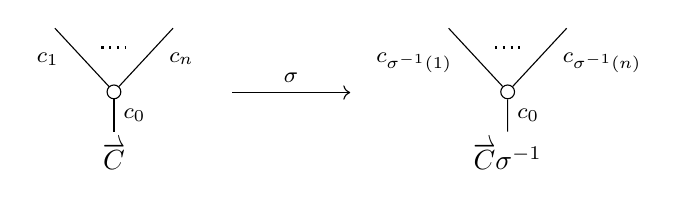
\begin{tikzpicture}
      [grow=up,auto,level distance=2.3em,every node/.style = {font=\footnotesize},dummy/.style={circle,draw,inner sep=0pt,minimum size=1.75mm}]
      
      \node at (0,0) [font=\normalsize]{$\vect{C}$}
		child{node [dummy] {}
			child{
			edge from parent node [swap,near end] {$\mathfrak c_n$} node [name=Kn] {}}
			child{
			edge from parent node [near end] {$\mathfrak c_1$}
node [name=Kone,swap] {}}
		edge from parent node [swap] {$\mathfrak c_0$}
		};
		\draw [dotted,thick] (Kone) -- (Kn) ;
	\node at (5,0) [font=\normalsize] {$\vect{C} \sigma^{-1}
	$}
		child{node [dummy] {}
			child{
			edge from parent node [swap,near end] {$\mathfrak c_{\sigma^{-1}(n)}$} node [name=Kn] {}}
			child{
			edge from parent node [near end] {$\mathfrak c_{\sigma^{-1}(1)}$}
node [name=Kone,swap] {}}
		edge from parent node [swap] {$\mathfrak c_0$}
		};
		\draw [dotted,thick] (Kone) -- (Kn) ;

\draw[->] (1.5,0.8) -- node{$\sigma$} (3,0.8);
\end{tikzpicture}
\end{equation}
Given any map of colors $\varphi \colon \mathfrak{C} \to \mathfrak{D}$ there is a functor (abusively written)
$\varphi \colon \Sigma_{\mathfrak{C}} \to \Sigma_{\mathfrak{D}}$,
given by 
$\varphi (\mathfrak c_1, \dots, \mathfrak c_n; \mathfrak c_0) = (\varphi(\mathfrak c_1),\cdots,\varphi(\mathfrak c_n);\varphi(\mathfrak c_0))$. 
\end{definition}


\begin{remark}\label{GLOBSIG REM}
The notation $\vect{C} \sigma^{-1}$
in \eqref{CSYM EQ1},\eqref{CSYM EQ2}
reflects the fact that $\Sigma_n$
acts on the right on $\mathfrak{C}$-signatures of arity $n$
via 
$\vect{C} \sigma = (\mathfrak{c}_i)\sigma = 
(\mathfrak{c}_{\sigma(i)})$,
where we make the convention that $\sigma(0)=0$.
\end{remark}



\begin{remark}
If one regards $\mathfrak{C} \in \mathsf{Set}$
as a discrete category, 
following Notation \ref{SIGWR NOT} one has an identification 
of groupoids
$\Sigma_{\mathfrak{C}} = (\Sigma \wr \mathfrak{C}) \times \mathfrak{C}$,
where the 
$\Sigma \wr \mathfrak{C}$ factor accounts for the sources
$\mathfrak{c}_1,\cdots,\mathfrak{c}_n$ of a signature
and the $\mathfrak{C}$ factor accounts for the target 
$\mathfrak{c}_0$.
\end{remark}



\begin{notation}
We will (slightly abusively) write
$\Sigma_{\bullet} \to \mathsf{Set}$
for the Grothendieck construction (see Notation \ref{GROTHCONS NOT})
of the functor
$\mathsf{Set} \to \mathsf{Cat}$ given by
$\mathfrak{C} \mapsto \Sigma_{\mathfrak{C}}$.

More explicitly, 
the objects of $\Sigma_{\bullet}$
are the $\vect{C} \in \Sigma_{\mathfrak{C}}$ 
for some set of colors $\mathfrak{C}$
and an arrow from
$\vect{C} \in \Sigma_{\mathfrak{C}}$ to
$\vect{D} \in \Sigma_{\mathfrak{D}}$
over $\varphi \colon \mathfrak{C} \to \mathfrak{D}$
is an arrow
$\varphi \vect{C} \to \vect{D}$ in $\Sigma_{\mathfrak{D}}$.
\end{notation}


\begin{definition}
Let $\mathcal{V}$ be a category.
The category $\mathsf{Sym}_\bullet(\mathcal{V})$ of
\textit{symmetric sequences on $\mathcal{V}$} 
(on all colors) is the category with:
\begin{itemize}
\item objects given by pairs $(\mathfrak C, X)$ with
      $\mathfrak{C} \in \mathsf{Set}$ a set of colors and
      $X \colon \Sigma_{\mathfrak{C}}^{op} \to \mathcal{V}$ a functor;
\item arrows $(\mathfrak C, X) \to (\mathfrak D, Y)$ given by a map 
      $\varphi \colon \mathfrak{C} \to \mathfrak{D}$ of colors and a natural transformation $X \Rightarrow Y \varphi$ as below.
\begin{equation}
\begin{tikzcd}[row sep = tiny, column sep = 45pt]
                  \Sigma_{\mathfrak{C}}^{op} \arrow[dr, "X"{name=U}] 
                  \arrow{dd}[swap]{\varphi}
\\
	& \mathcal{V}
\\
                  |[alias=V]| \Sigma_{\mathfrak{D}}^{op} \arrow[ur, "Y"']
                  \arrow[Leftarrow, from=V, to=U,shorten >=0.25cm,shorten <=0.25cm]
\end{tikzcd}
\end{equation}
\end{itemize}
\end{definition}


\begin{remark}\label{SUBCATDOWNL REM}
Given a category $\V$, let $\Cat \downarrow^l \V$ denote the category with
objects given by functors $\mathcal{C} \to \V$,
and arrows from $\mathcal{C} \to \V$ to $\mathcal{D} \to \V$
given by pairs 
$(\varphi,\phi)$ with 
$\varphi \colon \mathcal{C} \to \mathcal{D}$ a functor and
$\phi$ a natural transformation
\begin{equation}\label{SUBCATDOWNL EQ}
\begin{tikzcd}[row sep = tiny, column sep = 45pt]
	\mathcal C \arrow{dr}[name=U]{} \arrow{dd}[swap]{\varphi}
\\
	& \mathcal{V}
\\
	|[alias=V]| \mathcal D \arrow{ur}[swap]{}
	\arrow[Leftarrow, from=V, to=U,shorten >=0.25cm,shorten <=0.25cm
    ,swap,"\phi"]
\end{tikzcd}
\end{equation}
Then $\mathsf{Sym}_{\bullet}(\mathcal{V})$ is naturally a (neither wide nor full) subcategory of the $\mathsf{Cat}\downarrow^l \mathcal{V}$.
\end{remark}



\begin{remark}\label{COLCHADJ REM}
We caution that 
$\mathsf{Sym}_{\bullet}(\V)$
is rather different from the presheaf category 
$\mathsf{Fun}(\Sigma_{\bullet}^{op},\V)$.

Instead, one should think of 
$\mathsf{Sym}_{\bullet}(\V)$
as a form of ``fibered presheaves''.
More precisely, 
one has a (split) Grothendieck fibration
$\mathsf{Sym}_{\bullet}(\V) \to \mathsf{Set}$
with fiber over 
$\mathfrak{C} \in \mathsf{Set}$
the presheaf category
$\Sym_{\mathfrak C}(\V)=
\mathsf{Fun}(\Sigma_{\mathfrak{C}}^{op},\mathcal{V})$.
Note that for any map
$\varphi \colon \mathfrak{C} \to \mathfrak{D}$
one has adjunctions
\begin{equation}\label{COLCHADJ EQ}
\varphi_! \colon \Sym_{\mathfrak C}(\V) 
\rightleftarrows 
\Sym_{\mathfrak D}(\V) \colon \varphi^{\**}
\end{equation}
where $\varphi^{\**}$
(resp. $\varphi_!$)
is precomposition with (left Kan extention along)
$\varphi\colon 
\Sigma^{op}_{\mathfrak{C}}
\to 
\Sigma^{op}_{\mathfrak{D}}
$
so that the Grothendieck fibration
$\mathsf{Sym}_{\bullet}(\V) \to \mathsf{Set}$
is also an opfibration. 
\end{remark}


\begin{remark}\label{SUBCOCART REM}
The forgetful functor $\mathsf{Cat} \downarrow^l \mathcal{V} \to \mathcal{V}$
remembering only the source category is likewise both a fibration and an opfibrations, 
with a diagram \eqref{SUBCATDOWNL EQ}
being a cartesian arrow if  $\phi$ an isomorphism
and cocartesian if it is a left Kan extension. 
\end{remark}


Building on Remark \ref{COLCHADJ REM},
one can define a fibered Yoneda embedding, as in the following,
where we abbreviate
$\mathsf{Sym}_{\bullet} = \mathsf{Sym}_{\bullet}(\mathsf{Set})$.

\begin{notation}\label{FIBYON NOT}
Let $\mathfrak{C} \in \mathsf{Set}$, $\vect{C} \in \Sigma_{\mathfrak{C}}$.
We write
$\Sigma_{\mathfrak{C}}[\vect{C}] 
\in \mathsf{Sym}_{\mathfrak{C}} = \mathsf{Set}^{\Sigma_{\mathfrak{C}}^{op}}$ for the representable presheaf
\[\Sigma_{\mathfrak{C}}[\vect{C}](-)
= \Sigma_{\mathfrak{C}}(-,\vect{C}).\]
Moreover, we define the \emph{fibered Yoneda embedding}
\begin{equation}\label{FIBYON EQ}
\Sigma_{\bullet} \xrightarrow{\Sigma_{\bullet}[-]} \mathsf{Sym}_{\bullet}
\end{equation}
as $\Sigma_{\mathfrak{C}}[\vect{C}]$
when evaluated on an object
$\vect{C} \in \Sigma_{\mathfrak{C}} \subset \Sigma_{\bullet}$
and, on an arrow 
$\varphi \vect{C} \to \vect{D}$
over $\varphi \colon \mathfrak{C} \to \mathfrak{D}$,
as the natural transformation
$\Sigma_{\mathfrak{C}}[\vect{C}]
\Rightarrow
\varphi^{\**}
\Sigma_{\mathfrak{D}}[\vect{D}]
$ given by the natural composites
\[\Sigma_{\mathfrak{C}}[\vect{C}](-)
= \Sigma_{\mathfrak{C}}(-,\vect{C})
\to 
\Sigma_{\mathfrak{D}}(\varphi(-),\varphi\vect{C})
\to
\Sigma_{\mathfrak{D}}(\varphi(-),\vect{D})
=
\varphi^{\**} \Sigma_{\mathfrak{D}}[\vect{D}](-).
\]
\end{notation}



\begin{proposition}\label{FIBYONPUSH PROP}
Let $\vect{C} \in \Sigma_{\mathfrak{C}}$,
$\varphi \colon \mathfrak{C} \to \mathfrak{D}$
be a map of colors and consider the adjunction \eqref{COLCHADJ EQ}.

Then the adjoint of the canonical map
$\Sigma_{\mathfrak{C}}[\vect{C}]
\to
\varphi^{\**}\Sigma_{\mathfrak{D}}[\varphi\vect{C}]$
in $\mathsf{Sym}_{\mathfrak{C}}$
is an isomorphism
$\varphi_{!} \Sigma_{\mathfrak{C}}[\vect{C}]
\xrightarrow{\simeq}
\Sigma_{\mathfrak{D}}[\varphi\vect{C}]$
in $\mathsf{Sym}_{\mathfrak{D}}$.
\end{proposition}


Alternatively, this result states that 
the fibered Yoneda $\Sigma_{\bullet}[-]$
preserves cocartesian arrows.


\begin{proof}
For $Y \in \mathsf{Sym}_{\mathfrak{D}}$, by the (usual) Yoneda lemma one has isomorphisms
\begin{equation}\label{TWOYON EQ}
\mathsf{Sym}_{\mathfrak{D}}
(\Sigma_{\mathfrak{D}}[\varphi \vect{C}],Y)
\simeq
Y(\varphi \vect{C})
\simeq
\mathsf{Sym}_{\mathfrak{C}}(\Sigma_{\mathfrak{C}}[\vect{C}],\varphi^{\**}Y)
\end{equation}
proving 
$\Sigma_{\mathfrak{D}}[\varphi \vect{C}] \simeq \varphi_! \Sigma_{\mathfrak{C}}[\vect{C}]$.
That this identification is adjoint to the canonical map
$\Sigma_{\mathfrak{C}}[\vect{C}]
\to
\varphi^{\**}\Sigma_{\mathfrak{C}}[\varphi\vect{C}]$
in $\mathsf{Sym}_{\mathfrak{C}}$
follows since this sends
$id_{\vect{C}}$ to $id_{\varphi\vect{C}}$
(and since these identities determine the isomorphisms in \eqref{TWOYON EQ}).
\end{proof}



Now let $G$ be a group. Writing 
$\mathsf{Sym}^G_\bullet(\mathcal{V})
=
\left(\mathsf{Sym}_\bullet(\mathcal{V})\right)^G$
for the category of $G$-objects
in $\mathsf{Sym}_{\bullet}(\V)$,
the abstract nonsense argument in Remark \ref{FUNISGROTH REM}
yields that
$\mathsf{Sym}^G_\bullet(\mathcal{V}) \to \mathsf{Set}^G$
is again a Grothendieck fibration.
For each $\mathfrak{C} \in \mathsf{Set}^G$
we will then write
$\mathsf{Sym}^G_{\mathfrak{C}}(\V)$
to denote the fiber of
$\mathsf{Sym}^G_\bullet(\mathcal{V}) \to \mathsf{Set}^G$
over $\mathfrak{C}$.
We caution that 
$\mathsf{Sym}^G_{\mathfrak{C}}(\V)$
\emph{is not}
the category 
$\left(\mathsf{Sym}_{\mathfrak{C}}(\V)\right)^G$
of $G$-objects in $\mathsf{Sym}_{\mathfrak{C}}(\V)$
unless the $G$-action on $\mathfrak{C}$
happens to be trivial.

We will thus find it convenient to have a more explicit description of
$\mathsf{Sym}^G_{\mathfrak{C}}(\V)$,
provided by the following result, 
which is a slight strengthening of
\cite[Lemma A.6]{BP_geo}.
In fact, we prove a slightly more general description
for the categories $\mathsf{Cat} \downarrow^l \mathcal{V}$
in Remark \ref{SUBCATDOWNL REM},
for which the natural ``source category'' functor
$\mathsf{Cat} \downarrow^l \mathcal{V} \to \mathsf{Cat}$
is likewise a split Grothendieck fibration
with fiber over $\mathcal{C} \in \mathsf{Cat}$
given by
$\mathsf{Fun}(\mathcal{C},\mathcal{V})$.



\begin{proposition}\label{EQUIVFNCON PROP}
Let $G$ be a group and $\mathfrak{C} \in \mathsf{Set}^G$
be a $G$-set. Then there is a natural identification
\[
\mathsf{Sym}^G_{\mathfrak{C}}(\V)
\simeq
\mathsf{Fun}(G \ltimes \Sigma^{op}_{\mathfrak{C}},\V).
\]
More generally, 
for a category $\mathcal{B}$
the fiber of
$\left(\mathsf{Cat} \downarrow^l \V \right)^{\mathcal{B}}
\to \mathsf{Cat}^{\mathcal{B}}$
over a functor
$\mathcal{B} \xrightarrow{b \mapsto \mathcal{C}_b} \mathsf{Cat}$
is given by
\begin{equation}\label{FUNBLTICV EQ}
\mathsf{Fun}(\mathcal{B} \ltimes \mathcal{C}_{\bullet},\V).
\end{equation}
%\begin{equation}
%	\begin{tikzcd}
%		&
%		\mathsf{Sym}(\mathcal{V}) \arrow{d}{\mathsf{fgt}}
%&
%		&
%		\mathsf{Cat}\downarrow^l \mathcal{V} \arrow{d}{\mathsf{fgt}}
%\\
%		G \arrow{r}[swap]{\mathfrak{C}} \arrow[dashed]{ru} &
%		\mathsf{Set}
%&
%		\mathcal{D} \arrow{r}[swap]{\mathcal{C}_{\bullet}} \arrow[dashed]{ru} &
%		\mathsf{Cat}
%	\end{tikzcd}
%\end{equation}
\end{proposition}



\begin{proof}
It is immediate from the definitions that
$\mathsf{Sym}^G_{\mathfrak{C}}(\C)$
matches the fiber of 
$\left(\mathsf{Cat} \downarrow^l \V \right)^{G}
\to \mathsf{Cat}^{G}$
over $\Sigma_{\mathfrak{C}}^{op} \in \mathsf{Cat}^G$,
so we need only address the general case.

As in Notation \ref{GROTHCONS NOT},
let us write $\varphi_! \colon \mathcal{C}_b \to \mathcal{C}_{b'}$
for the functor induced by the arrow 
$\varphi_! \colon b \to b'$
in $\mathcal{B}$.
Unpacking definitions, an object of 
$\left(\mathsf{Cat} \downarrow^l \V \right)^{\mathcal{B}}$
over 
$\mathcal{C}_{\bullet} \colon \mathcal{B} \to \mathsf{Cat}$
corresponds to the data of functors
$\gamma_b \colon \mathcal{C}_b \to \mathcal{V}$ for each $b \in \mathcal{B}$
and natural transformations
$\phi_{\varphi} \colon \gamma_b \Rightarrow \gamma_{b'} \varphi_!$
for each $\varphi \colon b \to b'$ in $\mathcal{B}$
\begin{equation}\label{EQUIVFUNEX EQ}
\begin{tikzcd}[row sep = tiny, column sep = 50pt]
		\mathcal{C}_{b} \arrow{dr}[name=U]{\gamma_b} \arrow{dd}[swap]{\varphi_!}
	\\
		& \mathcal{V}
	\\
		|[alias=V]| \mathcal{C}_{b'} \arrow{ur}[swap]{\gamma_{b'}}
	\arrow[Leftarrow, from=V, to=U,shorten >=0.25cm,shorten <=0.25cm
	,swap,"\phi_{\varphi}"
	]
\end{tikzcd}
\end{equation}
subject to the requirements that
$\gamma_b \overset{\phi_{\varphi}}{\Rightarrow}
\gamma_{b'} \varphi_!
\overset{\phi_{\psi}\varphi_!}{\Rightarrow}
\gamma_{b'} \varphi_! \psi_!
$
equals 
$\gamma_b \overset{\phi_{\psi\varphi}}{\Rightarrow}
\gamma_{b'} \varphi_! \psi_!
$
for composable $b \xrightarrow{\varphi} b' \xrightarrow{\psi} b''$
and that
$\phi_{id_b} = id_{\gamma_b}$.

We now claim that the data above is exactly the data of a functor
$F \colon \mathcal{B} \ltimes \mathcal{C}_{\bullet} \to \mathcal{V}$.
To ease notation, we follow
Remark \ref{GROTHUNPCK REM}
and describe arrows in 
$\mathcal{B} \ltimes \mathcal{C}_{\bullet}$
as composites
$c \rightsquigarrow \varphi_! c \xrightarrow{f} c'$.
On fiber arrows 
$f\colon c \to c'$ in $\mathcal{C}_b$
set $F(f) = \gamma_b(f)$
and on cocartesian arrows set
$F(c \rightsquigarrow \varphi_! c) =
(\phi_{\varphi})_c$.
Then:
\begin{enumerate*}[label=(\roman*)]
\item
associavity and unitality of $F$ with respect to fiber arrows is equivalent to associativity and unitality of the $\gamma_b$;
\item associavity and unitality of $F$ with respect to the cocartesian arrows is equivalent to the conditions following 
\eqref{EQUIVFUNEX EQ};
\item $F$ respecting the commutative squares \eqref{GROTHUNPCK EQ}
is equivalent to naturality of the $\phi_{\varphi}$.
\end{enumerate*}

This finishes the proof that \eqref{FUNBLTICV EQ} has the correct set of objects. The claim that it also has the correct arrows is similar.
\end{proof}



Following the previous result, 
we will represent $G$-equivariant symmetric sequences
$X \in \mathsf{Sym}^G_{\mathfrak{C}}(\mathcal{V})$
for some $\mathfrak{C} \in \mathsf{Set}^G$
as functors
$X \colon G \ltimes \Sigma_{\mathfrak{C}}^{op} \to \mathcal{V}$.

Similarly, objects of
$\left( \mathsf{Cat} \downarrow^{l} \mathcal{V} \right)^G$
are represented by functors $G \ltimes \mathcal{C} \to \V$.


\begin{remark}\label{RHOPURP REM}
Recall that if $\mathcal{C}\in \mathsf{Cat}^G$
is a category with a $G$-action then 
$\Sigma \wr \mathcal{C}$
has a $G$-action where $G$ acts diagonally on tuples $(c_i)$ with $c_i \in \mathcal{C}$.
Therefore, by applying the 
$\Sigma \wr (-)$
construction to the categories
$\mathsf{Cat} \downarrow^l \V$
in Remark \ref{SUBCATDOWNL REM}
(note that that one can apply $\Sigma \wr (-)$
to the entirety of diagram \eqref{SUBCATDOWNL REM})
one obtains a description of the functor
\begin{equation}\label{RHOPURP EQ}
\begin{tikzcd}[column sep =40,row sep =0]
	\left( \mathsf{Cat} \downarrow^{l} \mathcal{V} \right)^G
	\ar{r}{\Sigma \wr (-) } &
	\left( \mathsf{Cat} \downarrow^{l} \Sigma \wr \mathcal{V} \right)^G
\\
	G \ltimes \mathcal{C} \to \mathcal{V} \ar[mapsto]{r} &
	\left(G \ltimes (\Sigma \wr \mathcal{C}) \to 
	\Sigma \wr (G \ltimes  \mathcal{C}) \to \Sigma \wr \mathcal{V}\right)
\end{tikzcd}
\end{equation}
where the natural functor
$G \ltimes (\Sigma \wr \mathcal{C}) \to 
\Sigma \wr (G \ltimes  \mathcal{C})$
is the inclusion described in Remark \ref{WRDIAG REM}.
\end{remark}


Since  
$\mathsf{Sym}^G_{\mathfrak{C}}(\mathcal{V}) \simeq 
\V^{G \ltimes \Sigma^{op}}$ is again a functor category, 
we will find it useful to discuss representable functors.
In the following discussion 
we set $\V = \mathsf{Set}$ and abbreviate
$\mathsf{Sym}^G_{\mathfrak{C}} = \mathsf{Sym}^G_{\mathfrak{C}}(\mathsf{Set})$.

As the objects of 
$G \ltimes \Sigma^{op}_{\mathfrak{C}}$
are simply the signatures
$\vect{C} \in \Sigma_{\mathfrak{C}}$,
each such signature induces a representable functor
$\left(G \ltimes \Sigma^{op}_{\mathfrak{C}}\right)(\vect{C},-)$
in 
$\mathsf{Sym}^G_{\mathfrak{C}}$.
However, caution is needed.
If one forgets the $G$-action on $\mathfrak{C}$,
then $\vect{C} \in \Sigma_{\mathfrak{C}}$
likewise induces the representable functor 
$\Sigma_{\mathfrak{C}}[\vect{C}]=\Sigma^{op}_{\mathfrak{C}}(\vect{C},-)$
in 
$\mathsf{Sym}_{\mathfrak{C}}$
as discussed in Notation \ref{FIBYON NOT}.
%
As such, our next task is to understand the relation between 
$\left(G \ltimes \Sigma^{op}_{\mathfrak{C}}\right)(\vect{C},-)$
and 
$\Sigma_{\mathfrak{C}}[\vect{C}]$
in such a way that we have analogues of the 
fibered Yoneda \eqref{FIBYON EQ}
and Proposition \ref{FIBYONPUSH PROP}.


As in our previous work in 
\cite[Not. 5.56]{Per18}, \cite[\S 2.3]{BP_edss}
the key to achieve this will be to extend the
$\Sigma_{\mathfrak{C}}[\vect{C}]$
notation to be defined not only for corollas $\vect{C}$
but also for ``colored forests of corollas''.
In fact, we will do a little more. 
In anticipation of our discussion of operads, 
we will extend this notation by defining 
$\Sigma_{\mathfrak{C}}[\vect{F}]$
for $\vect{F}$ a general colored forest (of trees).


\begin{definition}\label{COLFOR DEF}
Let $\mathfrak{C}$ be a set of colors.
The category $\Phi_{\mathfrak{C}}$ of $\mathfrak{C}$-colored forests has
\begin{itemize}
\item objects pairs
$\vect{F} = (F,\mathfrak{c})$
where 
$F\in \Phi$ is a forest
and 
$\mathfrak{c}\colon \boldsymbol{E}(F) \to \mathfrak{C}$ 
is a coloring of its edges;
\item a map
$\vect{F}=(F,\mathfrak{c}) \to 
(F',\mathfrak{c}') = \vect{F'}$
is a map $\rho \colon F \to F'$ in $\Phi$
such that
$\mathfrak{c} = \mathfrak{c}' \rho$.
\end{itemize}
If $\varphi\colon \mathfrak{C} \to \mathfrak{D}$ is a map of colors,
we write
$\varphi \colon \Phi_{\mathfrak{C}} \to \Phi_{\mathfrak{D}}$
for the functor sending 
$\vect{F} = (F,\mathfrak{c})$
to 
$\varphi\vect{F} = (F,\varphi\mathfrak{c})$.
Note that this defines a Grothendieck opfibration
\begin{equation}\label{PHIBGRO EQ}
\Phi_{\bullet} \to \mathsf{Set}
\end{equation}
whose objects are the $\vect{F} \in \Phi_{\mathfrak{C}}$ for some
$\mathfrak{C} \in \mathsf{Set}$
and with an arrow
from $\vect{F}$ to $\vect{F'}$
over
$\varphi \colon \mathfrak{C} \to \mathfrak{D}$
given by an arrow
$\varphi \vect{F} \to \vect{F'}$ in $\Phi_{\mathfrak{D}}$.
\end{definition}


For each vertex $v \in \boldsymbol{V}(F)$
in a forest, 
we write $F_v$ for the associated corolla.
Note that given a $\mathfrak{C}$-coloring $\vect{F}$ on $F$
one one likewise obtains colorings
$\vect{F}_v$ on $F_v$.



\begin{notation}
Given $\vect{F} \in \Phi_{\mathfrak{C}}$
we define
\begin{equation}\label{GENSIGC EQ}
\Sigma_{\mathfrak{C}}[\vect{F}]=
\coprod\nolimits^{\mathfrak{C}}_{v \in \boldsymbol{V}(F)} 
\Sigma_{\mathfrak{C}}[\vect{F}_v]
\end{equation}
where we highlight that the coproduct $\amalg^{\mathfrak{C}}$ is fibered, i.e. it takes place in $\mathsf{Sym}_{\mathfrak{C}}$
rather than $\mathsf{Sym}_{\bullet}$.
\end{notation}




\begin{example}\label{COLFORES EX}
Let 
$\mathfrak{C} = \{ \mathfrak{a}, \mathfrak{b}, \mathfrak{c} \}$.
On the left below we depict a $\mathfrak{C}$-colored forest 
$\vect{F} = \vect{T} \amalg \vect{S}$
with tree components $\vect{T},\vect{S}$.
\begin{equation}
	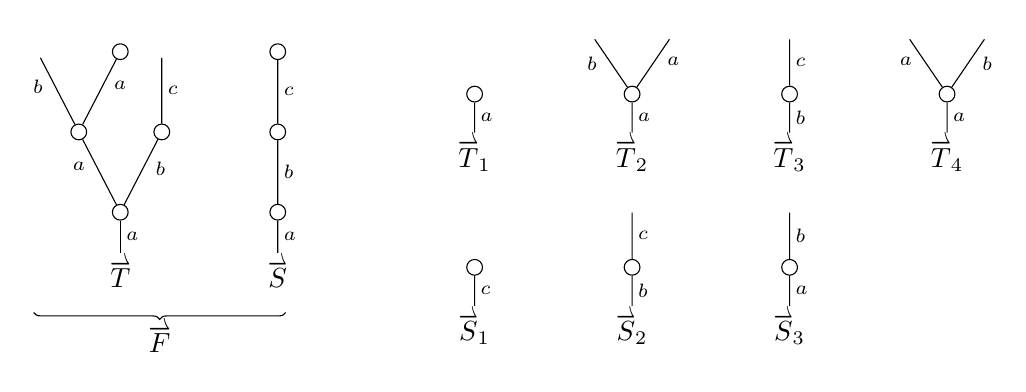
\begin{tikzpicture}[auto,grow=up, level distance = 2.2em,
	every node/.style={font=\scriptsize,inner sep = 2pt}]%
		\tikzstyle{level 2}=[sibling distance=3em]%
			\node at (0,0) [font = \normalsize] {$\vect{T}$}%	
				child{node [dummy] {}%
					child[level distance = 2.9em]{node [dummy] {}%
						child{node {}%
						edge from parent node [swap] {$\mathfrak{c}$}}%
					edge from parent node [swap,near end] {$\mathfrak{b}$}}%
					child[level distance = 2.9em]{node [dummy] {}%
						child[level distance = 2.9em]{node [dummy] {}%
						edge from parent node [swap,	near end] {$\mathfrak{a}$}}%
						child[level distance = 2.9em]{node {}%
						edge from parent node [near end] {$\mathfrak{b}$}}%
					edge from parent node [near end] {$\mathfrak{a}$}}%
				edge from parent node [swap] {$\mathfrak{a}$}};%
			\node at (2,0) [font = \normalsize] {$\vect{S}$}%	
				child{node [dummy] {}%
					child[level distance = 2.9em]{node [dummy] {}%
						child{node [dummy] {}%
						edge from parent node [swap] {$\mathfrak{c}$}}%
					edge from parent node [swap] {$\mathfrak{b}$}}%
				edge from parent node [swap] {$\mathfrak{a}$}};%
			\node at (4.5,1.5) [font = \normalsize] {$\vect{T}_1$}%	
				child{node [dummy] {}%
				edge from parent node [swap] {$\mathfrak{a}$}};%
			\node at (6.5,1.5) [font = \normalsize] {$\vect{T}_2$}%	
				child{node [dummy] {}%
					child{node {}%
					edge from parent node [swap, near end] {$\mathfrak{a}$}}%
					child{node {}%
					edge from parent node [near end] {$\mathfrak{b}$}}%
				edge from parent node [swap] {$\mathfrak{a}$}};%
			\node at (8.5,1.5) [font = \normalsize] {$\vect{T}_3$}%	
				child{node [dummy] {}%
					child{node {}%
					edge from parent node [swap] {$\mathfrak{c}$}}%
				edge from parent node [swap] {$\mathfrak{b}$}};%
			\node at (10.5,1.5) [font = \normalsize] {$\vect{T}_4$}%	
				child{node [dummy] {}%
					child{node {}%
					edge from parent node [swap, near end] {$\mathfrak{b}$}}%
					child{node {}%
					edge from parent node [near end] {$\mathfrak{a}$}}%
				edge from parent node [swap] {$\mathfrak{a}$}};%
			\node at (4.5,-0.7) [font = \normalsize] {$\vect{S}_1$}%	
				child{node [dummy] {}%
				edge from parent node [swap] {$\mathfrak{c}$}};%
			\node at (6.5,-0.7) [font = \normalsize] {$\vect{S}_2$}%	
				child{node [dummy] {}%
					child{node {}%
					edge from parent node [swap] {$\mathfrak{c}$}}%
				edge from parent node [swap] {$\mathfrak{b}$}};%
			\node at (8.5,-0.7) [font = \normalsize] {$\vect{S}_3$}%	
				child{node [dummy] {}%
					child{node {}%
					edge from parent node [swap] {$\mathfrak{b}$}}%
				edge from parent node [swap] {$\mathfrak{a}$}};%
		\draw[decorate,decoration={brace,amplitude=2.5pt}] (2.1,-0.5) -- (-1.1,-0.5) 
		node[midway,inner sep=4pt,font=\normalsize]{$\vect{F}$}; %
	\end{tikzpicture}%
\end{equation}%
Moreover, on the right we depict the $\mathfrak{C}$-signatures/corollas
$\vect{T}_i$ and $\vect{S}_j$
corresponding to the vertices of $T,S$ so that
\[
\Sigma_{\mathfrak{C}}[\vect{F}]=
\Sigma_{\mathfrak{C}}[\vect{T}] 
\amalg^{\mathfrak{C}}
\Sigma_{\mathfrak{C}}[\vect{S}]=
\left(
\coprod_{1\leq i \leq 4}^{\mathfrak{C}}
\Sigma_{\mathfrak{C}}[\vect{T}_i] 
\right)
\amalg^{\mathfrak{C}}
\left(
\coprod_{1\leq j \leq 3}^{\mathfrak{C}}
\Sigma_{\mathfrak{C}}[\vect{S}_j]
\right)
\]
\end{example}





\begin{remark}
The representables $\Sigma_{\mathfrak{C}}[-]$ in \eqref{GENSIGC EQ}
do not quite define a full functor on $\Phi_{\bullet}$
due to the fact that the only maps of forests 
sending vertices to vertices are the outer maps.
Writing $\Phi^o_{\bullet} \hookrightarrow \Phi_{\bullet}$
for the wide subcategory of those arrows whose underlying maps of uncolored forests are outer,
one has that \eqref{FIBYON EQ}
extends to give generalized fibered Yoneda embeddings
(where the right functor is obtained from the left functor by taking $G$-objects)
\[
\Phi_{\bullet}^o 
\xrightarrow{\Sigma_{\bullet}[-]}
\mathsf{Sym}_{\bullet},
\qquad
\Phi_{\bullet}^{o,G}
\xrightarrow{\Sigma_{\bullet}[-]}
\mathsf{Sym}^G_{\bullet}
\]
which are fibered over $\mathsf{Set}$ and $\mathsf{Set}^G$, respectively.
Note that Proposition \ref{FIBYONPUSH PROP} automatically generalizes, i.e. one has natural identifications
\begin{equation}\label{PUSHEQAG EQ}
\varphi_! \Sigma_{\mathfrak{C}}[\vect{F}] \simeq 
\Sigma_{\mathfrak{D}}[\varphi \vect{F}]
\end{equation}
for each map of colors
$\varphi \colon \mathfrak{C} \to \mathfrak{D}$
(which is an equivariant map in the equivariant case).
\end{remark}




\begin{notation}
We write $(-)^{\tau} \colon \Phi \to \Phi_{\bullet}$
for the \emph{tautological coloring} functor
which sends $F \in \Phi$ to 
$F^{\tau} \in \Phi_{\boldsymbol{E}(T)}$
where
$F^{\tau} = (F,\mathfrak{t})$ is the underlying forest $F$
together with the identity coloring
$\mathfrak{t} \colon \boldsymbol{E}(T) \xrightarrow{=} \boldsymbol{E}(T)$.
Moreover, we then abbreviate 
$\Sigma_{\tau}[F] = \Sigma_{\boldsymbol{E}(F)}[F^{\tau}]$.
\end{notation}


\begin{remark}
For any colored forest $\vect{F}=(F,\mathfrak{c})$,
regarding $\mathfrak{c} \colon \boldsymbol{E}(T) \to \mathfrak{C}$
as a change of color map, 
one has $\vect{F} = \mathfrak{c} F^{\tau}$,
so that \eqref{PUSHEQAG EQ} then yields that
\begin{equation}\label{CANPUSH EQ}
\Sigma_{\mathfrak{C}}[\vect{F}] = 
\mathfrak{c}_! \Sigma_{\tau}[F]
\end{equation}
\end{remark}


\begin{definition}
Let $G$ be a group,
$\mathfrak{C} \in \mathsf{Set}^G$
be a $G$-set of colors, 
and $\vect{C} \in \Sigma_{\mathfrak{C}}$ be a $\mathfrak{C}$-signature/corolla.
Write
$\vect{C} = (C,\mathfrak{c})$
with $C\in \Sigma$ the underlying corolla
and 
$\mathfrak{c} \colon \boldsymbol{E}(T) \to \mathfrak{C}$.

Writing 
$G \cdot \mathfrak{c} \colon G \cdot \boldsymbol{E}(T) \to \mathfrak{C}$
for the adjoint map, 
$G \in C \in \Phi^G$
for the $G$-free forest determined by $C$,
and noting that
$\boldsymbol{E}(G \cdot C) \simeq 
G \cdot \boldsymbol{E}(C)$
we define $G \cdot_{\mathfrak{C}} \vect{T} \in \Phi^G_{\mathfrak{C}}$ by
\begin{equation}\label{GCDTCC EQ}
G \cdot_{\mathfrak{C}} \vect{C} = 
(G \cdot \mathfrak{c})(G \cdot C)^{\tau}.
\end{equation}
\end{definition}



\begin{remark}
Regarding the $G$-action maps 
$g \colon \mathfrak{C} \to \mathfrak{C}$,
one has the more explicit formula
\[
G \cdot_{\mathfrak{C}} \vect{C}
= 
\coprod_{g \in G}
g \vect{C}
\]
However, in practice
we will prefer \eqref{GCDTCC EQ} for technical reasons.
\end{remark}


\begin{remark}
One can moreover extend \eqref{GCDTCC EQ}
to define a functor
$G \cdot_{\mathfrak{C}} (-) \colon \Phi_{\mathfrak{C}}
\to \Phi_{\mathfrak{C}}^G$
which is the left adjoint to the forgetful functor
$ \Phi_{\mathfrak{C}}^G
\to \Phi_{\mathfrak{C}}$.
\end{remark}


\begin{example}\label{GDOTCC EX}
Let $G = \{1,i,-1,-i\} \simeq \mathbb{Z}_{/4}$ 
be the group of quartic roots of unit and
$\mathfrak{C} = \{\mathfrak{a}, -\mathfrak{a}, i\mathfrak{a},-i,\mathfrak{a}, \mathfrak{b}, i \mathfrak{b} \}$ where we implicitly have
$-\mathfrak{b} = \mathfrak{b}$.
The following depicts the forest (of corollas) $G \cdot_{\mathfrak{C}} \vect{C}
$
for $\vect{C}$ the leftmost corolla.
\begin{equation}
	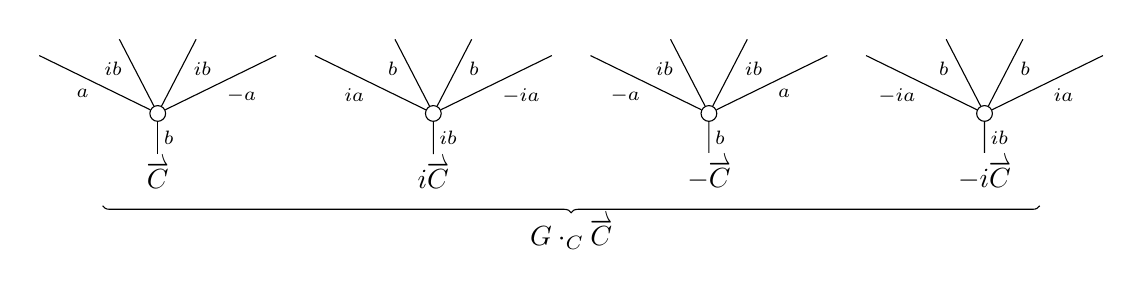
\begin{tikzpicture}[auto,grow=up, level distance = 2.2em,
	every node/.style={font=\scriptsize,inner sep = 2pt}]%
		\tikzstyle{level 2}=[sibling distance=3em]%
			\node at (0,0) [font = \normalsize] {$\vect{C}$}%	
				child{node [dummy] {}%
					child{node {}%
					edge from parent node [swap] {$-\mathfrak{a}$}}%
					child[level distance = 2.9em]{node {}%
					edge from parent node [swap,	near end] {$i\mathfrak{b}$}}%
					child[level distance = 2.9em]{node {}%
					edge from parent node [near end] {$i\mathfrak{b}$}}%
					child{node {}%
					edge from parent node  {$\mathfrak{a}$}}%
				edge from parent node [swap] {$\mathfrak{b}$}};%
			\node at (3.5,0) [font = \normalsize] {$i\vect{C}$}%	
				child{node [dummy] {}%
					child{node {}%
					edge from parent node [swap] {$-i\mathfrak{a}$}}%
					child[level distance = 2.9em]{node {}%
					edge from parent node [swap,	near end] {$\mathfrak{b}$}}%
					child[level distance = 2.9em]{node {}%
					edge from parent node [near end] {$\mathfrak{b}$}}%
					child{node {}%
					edge from parent node  {$i\mathfrak{a}$}}%
				edge from parent node [swap] {$i\mathfrak{b}$}};%
			\node at (7,0) [font = \normalsize] {$-\vect{C}$}%	
				child{node [dummy] {}%
					child{node {}%
					edge from parent node [swap] {$\mathfrak{a}$}}%
					child[level distance = 2.9em]{node {}%
					edge from parent node [swap,	near end] {$i\mathfrak{b}$}}%
					child[level distance = 2.9em]{node {}%
					edge from parent node [near end] {$i\mathfrak{b}$}}%
					child{node {}%
					edge from parent node  {$-\mathfrak{a}$}}%
				edge from parent node [swap] {$\mathfrak{b}$}};%
			\node at (10.5,0) [font = \normalsize] {$-i\vect{C}$}%	
				child{node [dummy] {}%
					child{node {}%
					edge from parent node [swap] {$i\mathfrak{a}$}}%
					child[level distance = 2.9em]{node {}%
					edge from parent node [swap,	near end] {$\mathfrak{b}$}}%
					child[level distance = 2.9em]{node {}%
					edge from parent node [near end] {$\mathfrak{b}$}}%
					child{node {}%
					edge from parent node  {$-i\mathfrak{a}$}}%
				edge from parent node [swap] {$i\mathfrak{b}$}};%
		\draw[decorate,decoration={brace,amplitude=2.5pt}] (11.2,-0.4) -- (-0.7,-0.4) 
		node[midway,inner sep=4pt,font=\normalsize]{$G \cdot_{\mathfrak{C}} \vect{C}$}; %
	\end{tikzpicture}%
\end{equation}%
Note that the pairs $\vect{C},-\vect{C}$
and $i\vect{C},-i\vect{C}$ are isomorphic in $\Sigma_{\mathfrak{C}}$
while any other pair such as, say, $\vect{C},i\vect{C}$ is not.
In general, it is moreover possible for two or more tree components of
$G \cdot_{\mathfrak{C}} \vect{C}$ to be equal.
\end{example}




\begin{proposition}\label{REPALTDESC PROP}
For any $G$-set of colors $\mathfrak C$
and $\mathfrak{C}$-signature
$\vect{C} \in \Sigma_{\mathfrak{C}}$
one has a natural identification
\[
(G \ltimes \Sigma^{op}_{\mathfrak{C}})(\vect{C},-)
\simeq 
\Sigma_{\mathfrak{C}} [G \cdot_{\mathfrak{C}} \vect{C}].
\]
\end{proposition}



\begin{proof}
Recalling the $C_{\varphi}(-,-)$ notation (cf. Notation \ref{MAPSDEC NOT})
for maps over $\varphi\colon b \to b'$ we likewise write 
$\mathsf{Sym}^G_{\varphi}(-,-),\mathsf{Sym}_{\varphi}(-,-)$
for maps over the map of colors $\varphi$.
The result now follows from the string of isomorphisms
(which show that $\vect{C}$ represents
$\Sigma_{\mathfrak{C}} [G \cdot_{\mathfrak{C}} \vect{C}] \in \mathsf{Set}^{G \ltimes \Sigma^{op}_{\mathfrak{C}}}$)
\[
	\mathsf{Sym}^G_{\mathfrak{C}}
	(\Sigma_{\mathfrak{C}} [G \cdot_{\mathfrak{C}} \vect{C}],X)
\simeq
	\mathsf{Sym}^G_{G \cdot \mathfrak{c}}
	(\Sigma_{\tau} [G \cdot C],X)
\simeq
	\mathsf{Sym}_{\mathfrak{c}}
	(\Sigma_{\tau} [C],X)
\simeq
	\mathsf{Sym}_{\mathfrak{C}}
	(\Sigma_{\mathfrak{C}}[\vect{C}],X)
=
	X(\vect{C})
\]
where: 
\begin{enumerate*}[label=(\roman*)]
\item the first and third steps 
use the canonical pushforwards \eqref{CANPUSH EQ}
and (the dual of) Remark \ref{CARTCHAR REM};
\item
the second step uses \eqref{ADJOVADJ EQ}
and the observation that
$\Sigma_{\tau}[G \cdot C] \simeq G \cdot \Sigma_{\tau}[C]$;
\item the last step is the Yoneda lemma in $\mathsf{Sym}_{\mathfrak{C}}$.
\end{enumerate*}
\end{proof}




We end this section by discussing convenient notation  
for subgroups 
$\Lambda \leq \mathsf{Aut}_{G \ltimes \Sigma_{\mathfrak{C}}^{op}}(\vect{C})$
of a $\mathfrak{C}$-signature $\vect{C}$
when regarded as an object of 
$G \ltimes \Sigma_{\mathfrak{C}}^{op}$.



\begin{remark}\label{SIGACT REM}
Extending Remark \ref{GLOBSIG REM}, 
the group $G \times \Sigma_n^{op}$
acts on the set $\Sigma_{\mathfrak{C},n}$
of $n$-ary $\mathfrak{C}$-signatures
$\vect{C} = (\mathfrak{c}_1,\cdots,\mathfrak{c}_n;\mathfrak{c}_0)$
via the assigment (where $g \in G$ acts on the left and $\sigma \in \Sigma_n$ on the right)
\begin{equation}\label{SIGACT_EQ}
	g \vect{C} \sigma =
	g (\mathfrak{c}_1,\cdots,\mathfrak{c}_n;\mathfrak{c}_0) \sigma
=
	(g\mathfrak{c}_{\sigma(1)},\cdots,g\mathfrak{c}_{\sigma(n)};g\mathfrak{c}_{\sigma(0)})
\end{equation}
or, more compactly, $g (\mathfrak{c}_i) \sigma = (g \mathfrak{c}_{\sigma(i)})$.

Moreover, the natural functor 
$G \ltimes \Sigma^{op}_{\mathfrak{C}}
\to G \times \Sigma^{op}$
which forgets colors is faithful,
with an arrow
$\vect{C} \to \vect{C'}$
between arity $n$ signatures
in $G \ltimes \Sigma_{\mathfrak{C}}^{op}$
given by 
$(g,\sigma) \in G \times \Sigma_n^{op}$
such that
$g \vect{C} \sigma = \vect{C'}$.
\end{remark}



\begin{remark}\label{GCDOTCATS REM}
If  $C \in \Sigma$ is the $n$-corolla
one has a natural identification
$\boldsymbol{E}(G\cdot C) = G \times \underline{n}_+$
where
$\underline{n}_+ = \{0,1,\cdots,n\}$.
The automorphisms of
$G \cdot C$ in $\Phi^G$
are then naturally identified with the group
$G^{op} \times \Sigma_n$,
with the automorphism
$G \cdot C \xrightarrow{(g,\sigma)} G \cdot C$
given on edges by
$(\bar{g},i) \mapsto (\bar{g}g,\sigma(i))$.
\end{remark}

 

\begin{remark}\label{COLCHSQ REM}
Let $g\vect{C} \sigma = \vect{C'}$
as in Remark \ref{SIGACT REM}.
Then $\vect{C},\vect{C'}$
have the same underlying corolla $C$ and, 
writing $\mathfrak{c},\mathfrak{c}'\colon 
\boldsymbol{E}(C)=\underline{n}_+ \to \mathfrak{C}$
for the colorings,
one can rewrite $g\vect{C} \sigma = \vect{C'}$
as 
$g \mathfrak{c} \sigma = \mathfrak{c}'$.

One then has a diagram below in $\Phi^G_{\bullet}$,
with the vertical maps given by the map 
$G \cdot C \xrightarrow{(g,\sigma)} G \cdot C$
in the underlying forest,
\begin{equation}\label{COLCHSQ EQ}
\begin{tikzcd}
G \cdot C^{\tau} \ar{d}[swap]{(g,\sigma)} 
\ar{r}{G \cdot \mathfrak{c}'}
&
G \cdot_{\mathfrak{C}} \vect{C'}
\ar{d}{(g,\sigma)}
\\
G \cdot C^{\tau} \ar{r}[swap]{G \cdot \mathfrak{c}}
&
G \cdot_{\mathfrak{C}} \vect{C}
\end{tikzcd}
\end{equation}
and where the right vertical map respects colors,
i.e. is a map in $\Phi^G_{\mathfrak{C}}$.
Note that this reflects Proposition \ref{REPALTDESC PROP},
which implies that a map $\vect{C} \to \vect{C'}$ in
$G \ltimes \Sigma_{\mathfrak{C}}^{op}$
is identified with a map 
$\Sigma_{\mathfrak{C}}[G \cdot_{\mathfrak{C}} \vect{C'}]
\to
\Sigma_{\mathfrak{C}}[G \cdot_{\mathfrak{C}} \vect{C}]$
in $\mathsf{Sym}^G_{\mathfrak{C}}$.
\end{remark}






\begin{example}
In Example \ref{GDOTCC EX}
the permutation $(14)(23) \in \Sigma_4$
gives a map $\vect{C} \to -\vect{C}$ in $\Sigma_{\mathfrak{C}}$
and thus induces an automorphism of
$\vect{C}$ in $G \ltimes \Sigma_{\mathfrak{C}}^{op}$.
\end{example}



\begin{definition}\label{STABS DEF}
If a subgroup $\Lambda \leq G \times \Sigma_n^{op}$
fixes a signature 
$\vect{C} = (\mathfrak{c}_1,\cdots,\mathfrak{c}_n;\mathfrak{c}_0)$,
i.e. if
$g\mathfrak{c}_{\sigma(i)} = \mathfrak{c}_i$
for all $(g, \sigma) \in \Lambda, 0 \leq i \leq n$,
we say that \textit{$\Lambda$ stabilizes $\vect C$}. 
% \emph{$\vect{C}$ and $\Lambda$ are compatible}.
\end{definition}



\begin{remark}\label{CHOOSESIGN REM}
For $\Lambda \leq G \times \Sigma_n^{op}$ 
the projection to $\Sigma_n^{op}$ yields a
right action of $\Lambda$ on 
$\underline{n}_+ = \{0,1,\cdots,n\}$.

Writing $\Lambda_i\leq \Lambda$ for the stabilizer of $i \in \underline{n}_{+}$ and $H_i = \pi_G(\Lambda_i)$
for its projection onto $G$,
one then has $H_i = g H_{\sigma(i)} g^{-1}$ for all
$(g, \sigma) \in \Lambda$.

Moreover, it readily follows that the 
signatures $\vect{C}$ that $\Lambda$ stabilizes
are in bijection with choices of 
$H_i$-fixed colors $\mathfrak{c}_i$ 
for $i$ ranging over a set of representatives of
the orbits $\underline{n}_+ /\Lambda$.
\end{remark}






\subsection{Equivariant colored symmetric operads}
\label{EQCOSYMOP SEC}

Our goal in this section is to describe the category 
$\mathsf{Op}^{G}_{\bullet}(\V)$
of equivariant colored operads.


We start by considering the non-equivariant case
$G = \**$,
for which we will describe
$\mathsf{Op}_{\bullet}(\V)$
as the category of fiber algebras over a certain fibered monad $\mathbb{F}$ on 
$\mathsf{Sym}_\bullet(\mathcal{V})$.

The restrictions of $\mathbb{F}$ to each fiber
$\mathsf{Sym}_{\mathfrak{C}}(\V)$,
i.e. the fiber monads $\mathbb{F}_{\mathfrak{C}}$,
are simply the ``free operad with set of objects $\mathfrak{C}$'' monads,
which are well known to be defined using 
$\mathfrak{C}$-colored trees.

\begin{definition}
      Let $\Omega_{\mathfrak C}$ denote the category of $\mathfrak C$-colored forests.
      \todo[inline]{add Definition \ref{COLFOR DEF}}

      $\Omega_{\mathfrak{C}} \subset \Phi_{\mathfrak{C}}$
      for the subcategory of $\mathfrak{C}$-colored forests which happen to be trees,
      as well as 
      $\Omega^0_{\mathfrak{C}} \subseteq \Omega_{\mathfrak{C}}$
      for the wide subcategory whose arrows are the isomorphisms.
\end{definition}




Next, following \cite[Notation 3.33]{BP_geo}
there is a ``colored arity functor''
\begin{equation}\label{LRDEF EQ}
\Omega_{\mathfrak C}^0 \xrightarrow{\mathsf{lr}_{\mathfrak C}} \Sigma_{\mathfrak{C}}
\end{equation}
which we call the \emph{leaf-root functor}, described as follows.
Given $\vect{T} \in \Omega^0_{\mathfrak{C}}$, 
its leaf-root
$\mathsf{lr}(\vect{T}) \in \Sigma_{\mathfrak{C}}$
is the only $\mathfrak{C}$-corolla
admitting a planar tall map
$\mathsf{lr}(\vect{T}) \to \vect{T}$,
where by ``tall map'' we mean a map
which sends leaves to leaves and the root to the root.


\begin{example}
For $\vect{T},\vect{S}$ the trees in Example \ref{COLFORES EX},
we depict $\mathsf{lr}(\vect{T})$, $\mathsf{lr}(\vect{S})$
which, informally, are obtained by keeping only the leaves and roots of those trees.
\begin{equation}
	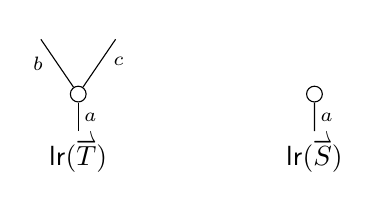
\begin{tikzpicture}[auto,grow=up, level distance = 2.2em,
	every node/.style={font=\scriptsize,inner sep = 2pt}]%
		\tikzstyle{level 2}=[sibling distance=3em]%
			\node at (0,0) [font = \normalsize] {$\mathsf{lr}(\vect{T})$}%	
				child{node [dummy] {}%
					child{node {}%
					edge from parent node [swap, near end] {$\mathfrak{c}$}}%
					child{node {}%
					edge from parent node [near end] {$\mathfrak{b}$}}%
				edge from parent node [swap] {$\mathfrak{a}$}};%
			\node at (3,0) [font = \normalsize] {$\mathsf{lr}(\vect{S})$}%	
				child{node [dummy] {}%
				edge from parent node [swap] {$\mathfrak{a}$}};%
	\end{tikzpicture}%
\end{equation}%
Alternatively, in signature notation we have
$\mathsf{lr}(\vect{T}) = (\mathfrak{b},\mathfrak{c};\mathfrak{a})$
and 
$\mathsf{lr}(\vect{S}) = (;\mathfrak{a})$.
\end{example}



\begin{remark}
Note that for a stick tree 
$\eta_{\mathfrak{c}}$
consisting of a single edge decorated by the color 
$\mathfrak{c} \in \mathfrak{C}$
it is 
$\mathsf{lr}(\eta_{\mathfrak{c}}) = (\mathfrak{c};\mathfrak{c})$,
which is the corolla with two edges (a leaf and a root) both labeled by $\mathfrak{c}$.
\end{remark}

\begin{remark}
      The colored leaf-root functor is in fact fibered over $\mathsf{Set}^G$:
      For any map of colors $\phi \colon \mathfrak C \to \mathfrak D$, we have
      the following commuting diagram.
      \begin{equation}
            \label{COLORLR_EQ}
            \begin{tikzcd}
                  \Omega_{\mathfrak C}^0 \arrow[r, "\phi"] \arrow[d, "\mathsf{lr}_{\mathfrak C}"']
                  &
                  \Omega_{\mathfrak D}^0 \arrow[d, "\mathsf{lr}_{\mathfrak D}"]
                  \\
                  \Sigma_{\mathfrak C} \arrow[r, "\phi"]
                  &
                  \Sigma_{\mathfrak D}
            \end{tikzcd}
      \end{equation}
\end{remark}

For each $\mathfrak{C}$-signature $\vect{C}$,
we write $\vect{C} \downarrow \Omega_{\mathfrak{C}}^0$
for the undercategory with respect to $\mathsf{lr}$, 
whose objects consist of a tree $\vect{T}\in \Omega_{\mathfrak{C}}^0$
together with a choice of isomorphism 
$\vect{C} \to \mathsf{lr}(\vect{T})$.
Morally, $\vect{C} \downarrow \Omega_{\mathfrak{C}}^0$
is the ``groupoid of trees with arity $\vect{C}$. 

We can now provide the ``usual'' formula for the ``free operad monad''
(see \cite[page 816]{BM07} for the non-colored case).
Letting 
$X \in \mathsf{Sym}_{\mathfrak{C}}(\V)$
then for each $\mathfrak{C}$-signature we have
\begin{equation}\label{FROPEXP EQ}
\mathbb{F}_{\mathfrak{C}} X (\vect{C})
=
\coprod_{[\vect{T}] \in 
\mathsf{Iso}(\vect{C} \downarrow \Omega^0_{\mathfrak{C}})}
\left(
\left(
\bigotimes_{v \in \boldsymbol{V}(T)} X(\vect{T}_v)
\right)
\cdot_{\mathsf{Aut}_{\Omega_{\mathfrak{C}}}(\vect{T})}
\mathsf{Aut}_{\Sigma_{\mathfrak{C}}}(\vect{C})
\right)
\end{equation}
where $\mathsf{Iso}(-)$ denotes isomorphism classes of objects.

However, one drawback of the formula  
\eqref{FROPEXP EQ}
is that it is not immediately clear how it should be modified 
in the equivariant case,
where $\mathfrak{C}$ is a $G$-set
and $X \in \mathsf{Sym}^G_{\mathfrak{C}}$
is a functor 
$X \colon G \ltimes \Sigma_{\mathfrak{C}}^{op} \to \V$.
To address this we first repackage \eqref{FROPEXP EQ}, 
following our approach in \cite[\S 4]{BP_geo}.
We first need to define another functor which we call the \emph{vertex functor}.
As motivation, we note that
in \eqref{FROPEXP EQ}
the $\mathsf{Aut}_{\Omega_{\mathfrak{C}}}(\vect{T})$-action
on the term
$\bigotimes_{v \in \boldsymbol{V}(T)} X(\vect{T}_v)$
depends on both permutations 
of the set $\boldsymbol{V}(T)$
and on automorphisms of the corollas $\vect{T}_v$.
As such, rather than regard the vertices of $\vect{T}$ as merely a set
we define 
\begin{equation}\label{VFUNDEF EQ}
\Omega_{\mathfrak{C}}^0 \xrightarrow{\boldsymbol{V}} \Sigma \wr \Sigma_{\mathfrak{C}}
\qquad 
\vect{T} \mapsto 
\boldsymbol{V}(\vect{T})=(\vect{T}_v )_{v \in \boldsymbol{V}(T)}
\end{equation}
In words, $\boldsymbol{V}(\vect{T})$
is the tuple of colored corollas indexed by the vertices of $T$. 
Note that
by regarding $\boldsymbol{V}(\vect{T})$ as an object in 
$\Sigma \wr \Sigma_{\mathfrak{C}}$ rather than just a set we can keep track of extra automorphism data.

Noting that both the leaf root and vertex functors are naturally compatible with change of colors 
$\varphi \colon \mathfrak{C} \to \mathfrak{D}$, 
we can now provide the following alternative 
description of \eqref{FROPEXP EQ}.



\begin{definition}\label{FREEOP DEF}
Let $\mathcal{V}$ be a closed symmetric monoidal category.

The \textit{fibered free operad monad} $\mathbb{F}$ on $\mathsf{Sym}_\bullet(\mathcal{V})$ 
assigns to 
$\Sigma_{\mathfrak{C}}^{op} \xrightarrow{X} \mathcal{V}$
the left Kan extension
\begin{equation}\label{FREEOP_EQ}
\begin{tikzcd}[column sep = 50pt]
	\Omega^{0,op}_{\mathfrak{C}}
	\arrow[d, "\mathsf{lr}^{op}"']
	\arrow[r, "\boldsymbol{V}^{op}"]
&
	(\Sigma \wr \Sigma_{\mathfrak{C}})^{op} \arrow[r, "(\Sigma \wr X^{op})^{op}"]
	\arrow[dl, Rightarrow]
&
	(\Sigma \wr \V^{op})^{op} \arrow[r, "\otimes"]
&
	\V
\\
	\Sigma^{op}_{\mathfrak{C}}
	\arrow[urrr, "\Lan = \mathbb F_{\mathfrak{C}} X = \mathbb F X"']
\end{tikzcd}
\end{equation}
\end{definition}
The complete discussion of the monad structure
$\mathbb{F}\mathbb{F} \Rightarrow \mathbb{F}$,
$id \Rightarrow \mathbb{F}$ is postponed to Appendix \ref{MONAD_APDX},
culminating in Definition \ref{COLORMON DEF}.


\begin{remark}\label{CONVER REM}
To relate \eqref{FROPEXP EQ} and \eqref{FREEOP_EQ} recall that 
for any span 
$\bar{\mathcal{G}} \overset{k}{\leftarrow} \mathcal{G} \xrightarrow{X} \mathcal{V}$
with $\mathcal{G},\bar{\mathcal{G}}$ groupoids
one has the formula
\[\Lan X (\bar{G}) \simeq 
\colim_{(k(g) \to \bar{g})\in (\mathcal{G} \downarrow \bar{g})} X(g) \simeq
\coprod_{[k(g) \to \bar{g}] 
\in \mathsf{Iso}(\mathcal{G} \downarrow \bar{g})}
\mathsf{Aut}_{\bar{\mathcal{G}}}(\bar{g})
\cdot_{\mathsf{Aut}_{\mathcal{G}}(g)}
X(g)
\]
where the second equality uses the observation that
$\mathcal{G} \downarrow \bar{g}$
is also a groupoid.
\end{remark}


By the abstract nonsense argument in 
Proposition \ref{DIAGRAMFM_PROP}
we have that, by taking $G$-objects, 
$\mathbb{F}$ also induces a fibered monad 
$\mathbb{F}^G$ on $\mathsf{Sym}^G_{\bullet}(\V)$.

To describe $\mathbb{F}^G$,
note that \eqref{FREEOP_EQ}
can be regarded as an arrow in 
the category $\mathsf{Cat} \downarrow^l \V$
from Remark \ref{SUBCATDOWNL REM}
which, being a left Kan extension, is cocartesian over $\mathsf{Cat}$ (cf. Remark \ref{SUBCOCART REM}).
Hence, if $X \in \mathsf{Sym}_{\bullet}^G(\V)$
is $G$-equivariant, 
\eqref{FREEOP_EQ} is then a cocartesian arrow in 
$\left(\mathsf{Cat} \downarrow^l \V\right)^G$
over $\mathsf{Cat}^G$.
By Proposition \ref{EQUIVFNCON PROP},
we can hence rewrite 
such a $G$-equivariant \eqref{FREEOP_EQ}
as the left Kan extension for a span
$G \ltimes \Sigma^{op}_{\mathfrak{C}}
\leftarrow 
G \ltimes \Omega^{0,op}_{\mathfrak{C}}
\to 
\V$.
To describe fully describe this span,
we need to understand how equivariance 
affects the top composite in \eqref{FREEOP_EQ},
with the non-obvious issue being that of understanding
what happens to the middle map
therein, which can be described using
Remark \ref{RHOPURP REM}.
Putting all of this together
(and using the isomorphisms
$G \ltimes \mathcal{C}^{op} \simeq (G \ltimes \mathcal{C})^{op}$
from Remark \ref{INVLTIMES REM})
we get the following.


\begin{proposition}\label{FGC PROP}
      The monad $\mathbb{F}^G$ on $\mathsf{Sym}^G_{\bullet}(\V)$
      assigns to 
      $G \ltimes \Sigma^{op}_{\mathfrak{C}} \xrightarrow{X} \V$
      the left Kan extension below.
\begin{equation}\label{FGC_EQ}
\begin{tikzcd}[column sep = 28pt]
	G \ltimes \Omega^{0,op}_{\mathfrak{C}}
	\arrow[d, "G \ltimes \mathsf{lr}_{\mathfrak C}^{op}"']
	\arrow[r, "G \ltimes \boldsymbol{V}^{op}"]
&[6pt]
	G \ltimes (\Sigma \wr \Sigma_{\mathfrak{C}})^{op} \arrow{r}
	\arrow[dl, Rightarrow, shorten >=0.15cm,shorten <=0.15cm]
&
	\left( \Sigma \wr \left( G^{op} \ltimes \Sigma_{\mathfrak{C}} \right) \right)^{op}
	\arrow[r, "(\Sigma \wr X^{op})^{op}"]
&[10pt]
	\left(\Sigma \wr \V^{op}\right)^{op} \arrow[r, "\otimes"]
&
	\V
\\
	G \ltimes \Sigma^{op}_{\mathfrak{C}}
	\arrow[urrrr, "\Lan = \mathbb F_{\mathfrak{C}}^G X = \mathbb F^G X"', end anchor = south west]
\end{tikzcd}
      \end{equation}
\end{proposition}







\begin{remark}\label{FROPEXPG REM}
By Remark \ref{CONVER REM} we now have the following analogue of
\eqref{FROPEXP EQ}.
\begin{equation}\label{FROPEXPG EQ}
\mathbb{F}^G_{\mathfrak{C}} X (\vect{C})
=
\coprod_{[\vect{T}] \in 
\mathsf{Iso}(\vect{C} \downarrow G^{op} \ltimes \Omega^0_{\mathfrak{C}})}
\left(
\left(
\bigotimes_{v \in \boldsymbol{V}(T)} X(\vect{T}_v)
\right)
\cdot_{\mathsf{Aut}_{G^{op} \ltimes \Omega_{\mathfrak{C}}}(\vect{T})}
\mathsf{Aut}_{G^{op} \ltimes \Sigma_{\mathfrak{C}}}(\vect{C})
\right)
\end{equation}
In comparing \eqref{FROPEXPG EQ} with \eqref{FROPEXP EQ} note that since 
$G^{op} \ltimes \Omega^0_{\mathfrak{C}}$
has more morphisms than
$\Omega^0_{\mathfrak{C}}$,
equation \eqref{FROPEXPG EQ} has less coproduct summands than \eqref{FROPEXP EQ},
though this is compensated by the fact that the inductions
$(-)\cdot_{\mathsf{Aut}_{G^{op} \ltimes \Omega_{\mathfrak{C}}}(\vect{T})}
\mathsf{Aut}_{G^{op} \ltimes \Sigma_{\mathfrak{C}}}(\vect{C})$
are correspondingly larger than the inductions
$(-)\cdot_{\mathsf{Aut}_{\Omega_{\mathfrak{C}}}(\vect{T})}
\mathsf{Aut}_{\Sigma_{\mathfrak{C}}}(\vect{C})$.
\end{remark}





\begin{remark}\label{OP_MAP REM}
      Following Remark \ref{ALGPUSHLL REM},
      for any map of $G$-sets 
      $\varphi \colon \mathfrak C \to \mathfrak D$
      and $\mathfrak D$-symmetric sequence $X$
      one has a pullback $\mathfrak C$-symmetric sequence $\varphi^{\**}X$
      given by
      $\varphi^{\**}X(\vect D) = X(\varphi(\vect D))$
      which is an operad if $X$ itself is an operad.
      Moreover, one then has a pair of adjunctions 
\begin{equation}\label{GC_CHANGE_EQ}
\begin{tikzcd}
	\Op^G_{\mathfrak C}(\V) 
	\arrow[shift left]{r}{\check{\varphi}_!}
	\arrow[d, "\mathsf{fgt}"']
&
	\Op^G_{\mathfrak D}(\V) 
	\arrow[shift left]{l}{\varphi^{\**}}
	\arrow[d, "\mathsf{fgt}"]
\\
	\Sym^G_{\mathfrak C}(\V) 
	\arrow[shift left]{r}{\varphi_!}
&
	\Sym^G_{\mathfrak D}(\V) 
	\arrow[shift left]{l}{\varphi^{\**}}
\end{tikzcd}
\end{equation}
      where we highlight that
      the right adjoints are compatible with the forgetful functors, in the sense that 
      $\varphi^{\**} \circ \mathsf{fgt} = 
      \mathsf{fgt} \circ \varphi^{\**}$, 
      but the left adjoints are not:
      $\varphi_!$ is simply a left Kan extension, while $\check{\varphi}_!$ is given by the coequalizer
\begin{equation}\label{CFS_EQ}
	\check{\varphi}_! \O \simeq \mathop{coeq}(\mathbb F_{\mathfrak D} \varphi_! \mathbb F_{\mathfrak C}\O \rightrightarrows \mathbb F_{\mathfrak D} \varphi_! \O).
\end{equation}
	In general, we can not give a more explicit description of $\check{\varphi}_!$.
	However, when $\varphi$ is injective, $\varphi_!X$ is simply 
	the extension by $\emptyset$
	from which it follows that 
	$\mathbb F_{\mathfrak D} \varphi_! = \varphi_! \mathbb F_{\mathfrak C}$,
	and \eqref{CFS_EQ}
	then says that
	$\check{\varphi}_! \O
	\simeq
	coeq \left( \varphi_! \mathbb{F}_{\mathfrak{C}}  \mathbb{F}_{\mathfrak{C}} \O
		\rightrightarrows 
	\varphi_!  \mathbb{F}_{\mathfrak{C}} \O
	\right)
	\simeq 
	\varphi_! \left( coeq \left( 
	\mathbb{F}_{\mathfrak{C}}  \mathbb{F}_{\mathfrak{C}} \O
	\rightrightarrows 
	\mathbb{F}_{\mathfrak{C}} \O
	\right) \right)
	\simeq 
	\varphi_! \O$,
	so that  	
	$\varphi_! \circ \mathsf{fgt} \simeq 
	\mathsf{fgt} \circ \check{\varphi}_!$.
	in this case.
\end{remark}




 
\subsection{Homotopy theory of operads with a fixed color $G$-set}
\label{OPC_MS_SEC}


We recall the fiber $\mathbb{F}^G_{\mathfrak{C}}$ from Proposition \ref{FGC PROP}
of the fibered monad $\mathbb{F}^G$.
% (and further fleshed out in {\color{red} Definition \ref{COLORMON DEF} (more detail needed)}).

Our goal in this section is to prove 
Theorem \ref{THMI} by transferring the $\F$-model structures on
$\mathsf{Sym}^G_{\mathfrak{C}}(\V)$
from Definition \ref{SYMGFV DEF}
to $\mathsf{Op}^G_{\mathfrak{C}}(\V)$
along the free-forgetful adjunction
\begin{equation}\label{OPAUTADJ EQ}
\mathbb{F}^G_{\mathfrak{C}} \colon
\mathsf{Sym}^G_{\mathfrak{C}}(\V)
\rightleftarrows
\mathsf{Op}^G_{\mathfrak{C}}(\V)
\colon \mathsf{fgt}
\end{equation}
so that a map in $\mathsf{Op}^G_{\mathfrak{C}}(\V)$
is a weak equivalence/fibration iff the underlying map in 
$\mathsf{Sym}^G_{\mathfrak{C}}(\V)$ is so.
%


The key to proving Theorem \ref{THMI} will be a suitable filtration of free operad extensions in $\mathsf{Op}_{\mathfrak{C}}^G(\V)$,
i.e. of pushouts as in \eqref{OURE EQ} below.
This filtration is given by Lemma \ref{OURE LEM},
whose proof is postponed to \S \ref{PUSHOUT_SEC} in the Appendix.
%culminating in Proposition \ref{FILTPUSHG PROP}.
The following discussion and lemma summarizes the properties of the filtration we will use.

We denote by $\Omega^a_{\mathfrak{C}}$
a variant of the category of trees, 
which we refer to as ``alternating trees''.
Its objects can be thought of as trees $\vect{T}$ 
whose set of vertices is partitioned into ``active'' and ``inert'' vertices,
$\boldsymbol{V}(\vect T) = 
\boldsymbol{V}^{ac}(\vect T) \amalg \boldsymbol{V}^{in}(\vect T)$,
in such a way that adjacent vertices are in different sides of the partition and the ``outer vertices'' (i.e. those adjacent to a leaf or root) are active.
Its maps are informally described as tall maps of trees that 
``send inert vertices to inert vertices''.



\begin{example}\label{ALTMAP EX}
	The following depicts an alternating map between alternating trees
	in $\Omega^a$.
	Active vertices are black $\bullet$ and inert vertives are white $\circ$.
	\[
	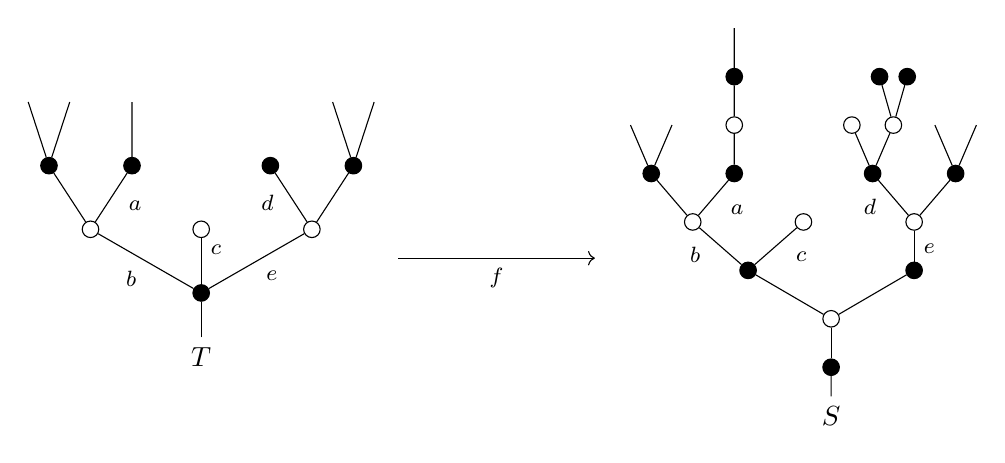
\begin{tikzpicture}[grow=up,auto,level distance=2.3em,every node/.style = {font=\footnotesize},dummy/.style={circle,draw,inner sep=0pt,minimum size=2.1mm}]
	\tikzstyle{level 2}=[sibling distance = 4em]
	\tikzstyle{level 3}=[sibling distance = 3em]
	\tikzstyle{level 4}=[sibling distance = 1.5em]
	\node at (0,0.75) [font = \normalsize] {$T$}
	child{node [dummy,fill = black] {}
		child{node [dummy,fill=white] {}
			child{node [dummy,fill = black] {}
				child
				child
			}
			child{node [dummy,fill = black] {}
				edge from parent node [near end] {$d$}}
			edge from parent node [swap] {$e$}}
		child{node [dummy,fill=white] {}
			edge from parent node [swap, near end] {$c$}}
		child{node [dummy,fill=white] {}
			child{node [dummy,fill = black] {}
				child
				edge from parent node [swap, near end] {$a\phantom{d}$}}
			child{node [dummy,fill = black] {}
				child
				child
			}
			edge from parent node {$b$}}
	};
	\begin{scope}[level distance=1.75em]
	\tikzstyle{level 3}=[sibling distance = 6em]
	\tikzstyle{level 4}=[sibling distance = 4em]
	\tikzstyle{level 5}=[sibling distance = 3em]
	\tikzstyle{level 6}=[sibling distance = 1.5em]
	\tikzstyle{level 7}=[sibling distance = 1em]
	\node at (8,0) [font = \normalsize] {$S$}
	child{node [dummy,fill = black] {}
		child{node [dummy,fill = white] {}
			child{node [dummy,fill = black] {}
				child{node [dummy,fill=white] {}
					child{node [dummy,fill = black] {}
						child
						child
					}
					child{node [dummy,fill = black] {}
						child{node [dummy,fill=white] {}
							child{node [dummy,fill = black] {}}
							child{node [dummy,fill = black] {}}
						}
						child{node [dummy,fill=white] {}}
						edge from parent node [near end] {$d$}}
					edge from parent node [swap] {$e\phantom{1}$}}
			}
			child{node [dummy,fill = black] {}
				child{node [dummy,fill=white] {}
					edge from parent node [swap, near end] {$c\phantom{1}$}}
				child{node [dummy,fill=white] {}
					child{node [dummy,fill = black] {}
						child{node [dummy,fill=white] {}
							child{node [dummy,fill = black] {}
								child
							}
						}
						edge from parent node [swap,near end] {$a\phantom{d}$}}
					child{node [dummy,fill = black] {}
						child
						child
					}
					edge from parent node [near end] {$\phantom{1}b$}}
			}
		}
	};
	\end{scope}
	\draw [->] (2.5,2) -- node [swap] {$f$} (5,2);
	\end{tikzpicture}
	\]
\end{example}




Furthermore, we write
$\Omega_{\mathfrak C}^a[k] \subseteq \Omega_{\mathfrak C}^a$
for the full subcategory of $\vect{T}$ such that 
$|\boldsymbol{V}^{in}(\vect{T})| = k$,
i.e. such that $\vect{T}$ has exactly $k$ inert vertices.
Crucially, $\Omega^a_{\mathfrak{C}}[k]$
turns out to be a groupoid.
%
Adapting \eqref{LRDEF EQ} and \eqref{VFUNDEF EQ}, 
we have functors
\[
\mathsf{lr}_{\mathfrak C}^{a} \colon
\Omega^a_{\mathfrak{C}}[k]
\to
\Sigma_{\mathfrak{C}}
	\qquad
\boldsymbol{V}^{in} \colon
\Omega^a_{\mathfrak{C}}[k]
\to
\Sigma_k \wr \Sigma_{\mathfrak{C}}
\]
where $\mathsf{lr}_{\mathfrak C}^{a}$ is defined as before (one just ignores the vertex partition data)
and $\boldsymbol{V}^{in}$ is the tuple containing only the inert vertices.



\begin{lemma}\label{OURE LEM}
Fix a $G$-set of colors $\mathfrak{C}$ and let
$u\colon X \to Y$ be a map in $\mathsf{Sym}^G_{\mathfrak{C}}(\V)$
and
$\mathbb{F} X \to \O$ be a map in $\mathsf{Op}^G_{\mathfrak{C}}(\V)$.
Then, for the pushout 
\begin{equation}\label{OURE EQ}
\begin{tikzcd}
	\mathbb F X \arrow[d, "\mathbb{F}u"'] \arrow[r]
&
	\O \arrow[d]
\\
	\mathbb F Y \arrow[r]
&
\O[u]
\end{tikzcd}
\end{equation}
in the category of operads $\mathsf{Op}^G_{\mathfrak{C}}(\V)$
the map $\O \to \O[u]$ admits an underlying filtration
\begin{equation}\label{OUFILRE EQ}
\O = \O_0 \to \O_1 \to \O_2 \to \cdots \to \O_{\infty} = \O[u]
\end{equation}
of maps in $\mathsf{Sym}^G_{\mathfrak{C}}(\V)$ 
where each map $\O_{k-1} \to \O_k$ fits into a pushout
\begin{equation}\label{OUPUSHRE EQ}
\begin{tikzcd}
	\bullet 
	\arrow{d}[swap]{\left(\mathsf{lr}_{\mathfrak C}^{a,op}\right)_!
	n_k^{(\O,X,Y)}}
	 \arrow[r]
&
	\O_{k-1} \arrow[d]
\\
	\bullet \arrow[r]
&
	\O_k
\end{tikzcd}
\end{equation}
where 
$
\left(\mathsf{lr}_{\mathfrak C}^{a,op}\right)_! \colon
\mathcal{V}^{G \ltimes \Omega^a_{\mathfrak{C}}[k]^{op}}
\to
\mathcal{V}^{G \ltimes \Sigma_{\mathfrak{C}}^{op}}
=
\mathsf{Sym}^G_{\mathfrak{C}}(\V)
$
is as in Proposition \ref{EQQUILADJ PROP}
and $n_k^{(\O,X,Y)}$ is the natural transformation in 
$\mathcal{V}^{G \ltimes \Omega^a_{\mathfrak{C}}[k]^{op}}$
whose constituent arrows for $\vect{T} \in \Omega^a_{\mathfrak C}[k]$ are
\begin{equation}\label{NKOXY EQ}
n_k^{(\O,X,Y)}(\vect{T})=
	\left(
		\bigotimes_{v \in \boldsymbol{V}^{ac}(\vect{T})}\O(\vect{T}_v)
	\otimes
		\mathop{\mathlarger{\mathlarger{\mathlarger{\square}}}}\limits_{v \in \boldsymbol{V}^{in}(\vect{T})} u(\vect{T}_v)
          \right)
          =
          \left(
                \mathop{\mathlarger{\mathlarger{\mathlarger{\square}}}}\limits_{v \in \boldsymbol{V}^{ac}(\vect{T})} \left( \emptyset \to \O(\vect{T}_v)\right) 
          \square
          \mathop{\mathlarger{\mathlarger{\mathlarger{\square}}}}\limits_{v \in \boldsymbol{V}^{in}(\vect{T})} u(\vect{T}_v)
          \right)
\end{equation}
\end{lemma}


We can now prove our first main result, Theorem \ref{THMI}.


\begin{proof}[Proof of Theorem \ref{THMI}]    
Writing
$\mathcal{I}_{\mathfrak{C},\mathcal{F}}$,
$\mathcal{J}_{\mathfrak{C},\mathcal{F}}$
for the generating sets
of the $\F$-model structure on 
$\mathsf{Sym}^G_{\mathfrak{C}}(\V)$
(cf. Remark \ref{VGSIGF REM}),
it is immediate by adjunction
that the desired transfer $\F$-model structure
on $\mathsf{Op}^G_{\mathfrak{C}}(\V)$
will have generating sets 
$\mathbb{F}^G_{\mathfrak{C}}\mathcal{I}_{\mathfrak{C},\mathcal{F}}$,
$\mathbb{F}^G_{\mathfrak{C}}\mathcal{J}_{\mathfrak{C},\mathcal{F}}$.
	 
By \cite[Thm. 11.3.2]{Hir03} we need only show that
all maps in
$(\mathbb{F}^G_{\mathfrak{C}}\mathcal{J}_{\mathfrak{C},\mathcal{F}})$-cell
are $\F$-weak equivalences in $\mathsf{Sym}^G_{\mathfrak{C}}(\V)$.
Moreover, since trivial $\F$-cofibrations are genuine trivial cofibrations and 
genuine weak equivalences are $\F$-weak equivalences, one needs only consider the genuine case, i.e. the case of $\F_{all}$ the family of all subgroups (this repeats the argument in \eqref{FAMTOGEN EQ}).


Since we are assuming $\V$ satisfies the global monoidal axiom, 
it is thus enough to show that pushouts of maps in 
$(\mathbb{F}^G_{\mathfrak{C}}\mathcal{J}_{\mathfrak{C},\mathcal{F}_{all}})$,
i.e. maps $\O \to \O[u]$ in \eqref{OURE EQ}
for $u \in \mathcal{J}_{\mathfrak{C},\mathcal{F}_{all}}$
are equivariant $\otimes$-trivial cofibrations
in $\mathsf{Sym}^G_{\mathfrak{C}}(\V) = \V^{G \ltimes \Sigma^{op}_{\mathfrak{C}}}$.



We thus now assume $u \in \mathcal{J}_{\mathfrak{C},\mathcal{F}_{all}}$.
Now note that for $\vect{T} \in \Omega^a_{\mathfrak{C}}[k]$
it is
\[
	\mathop{\mathlarger{\mathlarger{\mathlarger{\square}}}}\limits_{v \in \boldsymbol{V}^{in}(\vect{U})} u(\vect{T}_v)
=
	u^{\square k}\left( \boldsymbol{V}^{in}(\vect T) \right)
\]
where
$u^{\square k} \in 
\V^{\Sigma_k \wr (G \ltimes \Sigma^{op}_{\mathfrak{C}})}$
is as defined in \eqref{FSQNDEF EQ}.
By Proposition \ref{SIGMAWRGF PROP}
$u^{\square k}$ is a genuine trivial cofibration in 
$\V^{\Sigma_k \wr (G \ltimes \Sigma^{op}_{\mathfrak{C}})}$
so that by
Proposition \ref{EQQUILADJ PROP}
$u^{\square k}(\boldsymbol{V}^{in}(-))$
is similarly a genuine trivial cofibration in 
$\V^{G \ltimes \Omega^{a,op}_{\mathfrak{C}}[k]}$.
It is now clear that
the map $n_k^{(\O,X,Y)}$ in \eqref{NKOXY EQ}
is an equivariant
$\otimes$-trivial cofibration in 
$\V^{G \ltimes \Omega^{a,op}_{\mathfrak{C}}[k]}$,
so that by 
Proposition \ref{REGEOTCOF PROP}
the maps $\O_{k-1} \to \O_{k}$
in the pushouts \eqref{OUPUSHRE EQ}
are genuine $\otimes$-trivial cofibrations
in 
$\mathsf{Sym}^G_{\mathfrak{C}}(\V)
= \V^{G\ltimes \Sigma^{op}_{\mathfrak{C}}}$.
Thus the composite $\O \to \O[u]$
is also an
equivariant $\otimes$-trivial cofibration
and the result follows.
\end{proof}




For later reference, 
we highlight two consequences of the previous proof.


\begin{remark}\label{GOTC_REM}
$\F$-trivial cofibrations in $\Op^G_{\mathfrak C}(\V)$ are underlying genuine $\otimes$-trivial cofibrations
in $\mathsf{Sym}^G_{\mathfrak C}(\V)$.
\end{remark}

\begin{remark}
The generating (trivial) cofibrations in
$\mathsf{Op}^G_{\mathfrak{C},\F}(\V)$
are the sets
\begin{equation}\label{FVGSIGF EQ}
	\mathbb{F}^G_{\mathfrak{C}}\mathcal{I}_{\mathfrak{C},\mathcal{F}}
=
	\left\{
	\mathbb{F}^G_{\mathfrak{C}}
	\left(\Sigma_{\mathfrak{C}}[G \cdot_{\mathfrak{C}} \vect{C}]/\Lambda \cdot i \right)
	\right\}
\qquad \qquad
	\mathbb{F}^G_{\mathfrak{C}}\mathcal{I}_{\mathfrak{C},\mathcal{F}}
=
	\left\{
	\mathbb{F}^G_{\mathfrak{C}}
	\left(\Sigma_{\mathfrak{C}}[G \cdot_{\mathfrak{C}} \vect{C}]/\Lambda \cdot j \right)
	\right\}
\end{equation}
where $\vect{C}$ ranges over $\Sigma_{\mathfrak{C}}$,
$\Lambda$ ranges over $\F_{\vect{C}}$,
$i$ ranges over $\mathcal{I}$ and
$j$ ranges over $\mathcal{J}$.
\end{remark}



\begin{corollary}\label{OPADJ_COR}
\begin{enumerate}[label=(\roman*)]
\item \label{OPCOCHADJ_LBL}
	For any $(G,\Sigma)$-family $\F$ and map of colors 
	$\varphi \colon \mathfrak C \to \mathfrak D$, the induced adjunction
		\[
		\check{\varphi}_! \colon \mathsf{Op}^G_{\mathfrak{C},\F}
			\rightleftarrows
		\mathsf{Op}^G_{\mathfrak{D},\F} \colon \varphi^{\**}
		\]
	is a Quillen adjunction.
\item \label{OPFIXSETCHGR_LBL}
	For any homomorphism $\phi \colon G \to \bar G$,
	$(G,\Sigma)$-family $\F$ and $(\bar G,\Sigma)$-family $\bar{\F}$,
	and $\bar G$-set of colors $\bar{\mathfrak C}$,
	the adjunction
		\[
		\check{\phi}_! \colon \mathsf{Op}^G_{\bar{\mathfrak{C}},\F}
			\rightleftarrows
		\mathsf{Op}^{\bar{G}}_{\bar{\mathfrak{C}},\bar{\F}} \colon \phi^{\**}
		\]
	is a Quillen adjunction whenever $\F \subseteq \phi^{\**} \bar{\F}$.
\item \label{OPCOMBADJ_LBL}
	For any homomorphism $\phi \colon G \to \bar G$,
	$(G,\Sigma)$-family $\F$ and $(\bar G,\Sigma)$-family $\bar{\F}$,
	and $G$-set of colors $\mathfrak C$,
	the adjunction
            \[
                  \bar{G} \cdot_G (-) \colon \mathsf{Op}^G_{\mathfrak{C},\F}
                  \rightleftarrows
                  \mathsf{Op}^{\bar{G}}_{\bar{G} \cdot_G \mathfrak{C},\bar{\F}} \colon \mathsf{fgt}
            \]
	is a Quillen adjunction whenever $\F \subseteq \phi^{\**} \bar{\F}$.
      \end{enumerate}
\end{corollary}

\begin{proof}
	Since operadic weak equivalences, fibrations and the forgetful functors $\varphi^{\**},\phi^{\**}$
	are all defined in terms of the underlying symmetric sequences,
	this is immediate from Corollary \ref{SYMADJ_COR}.
\end{proof}






\begin{remark}\label{CSPNTHI REM}
When \eqref{OURE EQ}
is a diagram in $\mathsf{Cat}^G_{\mathfrak{C}}(\V)$, 
the map 
$n_k^{(\mathcal{O},X,Y)}(\vect{T})$
in \eqref{NKOXY EQ}
is necessarily $\emptyset \to \emptyset$
unless $\vect{T}$ is a linear tree.
But if $\vect{T}$ is linear
its automorphism group in 
$G \ltimes \Omega_{\mathfrak{C}}^{a,op}[k]$
is simply a subgroup of $G$
and does not permute the factors in \eqref{NKOXY EQ}.
Hence, the key claim in the proof of Theorem \ref{THMI} that 
$n_k^{(\mathcal{O},X,Y)}$
is an equivariant $\otimes$-trivial cofibration in
$\V^{G \ltimes \Omega_{\mathfrak{C}}^{a,op}[k]}$
follows by replacing the use of Proposition \ref{SIGMAWRGF PROP}
with the more elementary
Proposition \ref{RESGEN PROP},
and thus does not require
the cofibrant pushout powers condition
in Definition \ref{CSPP_DEF} and Theorem \ref{THMI}.
\end{remark}




\begin{remark}\label{THMISM REM}
	If $\O$ in \eqref{OURE EQ}
	is known to be underlying genuine cofibrant
	(i.e. $\F_{all}$-cofibrant) in 
	$\mathsf{Sym}^{G}_{\mathfrak{C}}(\V)$ 
	then, replacing the use of the global monoid axiom with 
	Proposition \ref{RESGEN PROP},
	the argument in the proof of Theorem \ref{THMI}
	shows that the maps
	$\O_{k-1} \to \O_k$
	and their composite
	$\O \to \O[u]$
	are genuine trivial cofibrations
	(rather than just genuine $\otimes$-trivial cofibrations).
	
	On the other hand, conditions (i),(ii),(iii),(iv) in Theorem \ref{THMI}
	suffice to show that if $\O$ is $\mathcal{F}_{all}$-cofibrant in 
	$\mathsf{Op}^G_{\mathfrak{C}}(\V)$
	then it is underlying $\mathcal{F}_{all}$-cofibrant in 
	$\mathsf{Sym}^G_{\mathfrak{C}}(\V)$
	(this follows either by the proof of Theorem \ref{THMII} in \S \ref{INDSYS SEC},
	or by repeating the argument in the proof of Theorem \ref{THMI} but now with $u \in \mathcal{I}_{\mathfrak{C},\F_{all}}$
	a generating cofibration).
	
	Therefore, by \cite[Thm. 2.2.2]{WY18},
	the semi-model structure analogue of Theorem \ref{THMI}
	does not require the global monoid axiom (v).
\end{remark}
  




\section{The monad for free colored operads}
\label{MONAD_APDX}

This appendix is fairly technical.
Its goal is to complete Definition \ref{FREEOP DEF}
by fully describing the monad structure 
on the fibered free operad monad $\mathbb{F}$
of \eqref{FREEOP_EQ},
and to use this to prove some technical results used in the rest of the paper, 
most notably the key filtration result in Lemma \ref{OURE LEM}.


Our approach builds off our previous work in \cite{BP_geo},
and is motivated by the fact that the left Kan extension in \eqref{FREEOP_EQ} makes the monad structure somewhat awkward to describe and work with directly.
As such, our strategy is to note that there is an adjunction 
\begin{equation}\label{SPANSYMADJ EQ}
\mathsf{Lan} \colon
\mathsf{WSpan}^l(\Sigma_{\bullet}^{op},\mathcal{V}) 
	\rightleftarrows
\mathsf{Sym}_{\bullet}(\mathcal{V})
\colon \iota
\end{equation}
that identifies $\mathsf{Sym}_{\bullet}(\V)$ 
as a reflexive subcategory of a larger category 
$\mathsf{WSpan}^l(\Sigma_{\bullet}^{op},\mathcal{V})$
of spans, with the left Kan extension being the reflection.
We then build a monad $N$ on the larger category 
$\mathsf{WSpan}^l(\Sigma_{\bullet}^{op},\mathcal{V})$
and show that this monad can be transferred to 
$\mathsf{Sym}_{\bullet}(\mathcal{V})$.




We begin by establishing technical definitions and relations which are the key constituents of the monad in \S \ref{CSTRINGS_SEC} and \S \ref{WRACONST SEC}.
In \S \ref{NONEQMON SEC}, we construct the monad describing colored operads $\Op(\V)$, as well as provide a useful filtration on free extensions of operads.
In \S \ref{EQMON_SEC}, we upgrade these discussions to the equivariant case.





\subsection{Colored strings}
\label{CSTRINGS_SEC}


We now recall and adapt many 
of the key notions from \cite{BP_geo}.

Firstly, just as in \S \ref{EQCOSYMOP SEC}
we write 
$\Omega_{\mathfrak{C}}$
for the category of 
$\mathfrak{C}$-colored trees
$\vect{T} = (T,\mathfrak{c}\colon \boldsymbol{E}(T) \to \mathfrak{C})$
and color preserving maps.

We will make use of certain special types of maps in $\Omega_{\mathfrak{C}}$, all of which are defined in terms of the underlying map of trees.
A map $f \colon \vect{T} \to \vect{S}$
is called:
\emph{planar} is the underlying map of trees is planar;
\emph{tall} if it sends leaves to leaves and the root to the root;
an \emph{outer face}
if for any factorization 
$f = f' t$ with $t$ a tall map one has that $t$ is an isomorphism. 

Any map $\vect{T} \xrightarrow{f} \vect{S}$ in $\Omega_{\mathfrak{C}}$
then has a factorization
$\vect{T} \xrightarrow{f^t} \vect{R} \xrightarrow{f^o} \vect{S}$,
unique up to unique isomorphism,
with $f^t$ a tall map and $f^o$ an outer map.
Moreover, this factorization is strictly unique if $f,f^o$ are required to be planar.

\begin{notation}
	Given a planar map $\vect{T} \to \vect{S}$
	and $v \in \boldsymbol{V}(T)$
	we write
	$\vect{T}_v \to \vect{S}_v \to \vect{S}$
	for the ``tall map followed by outer face''
	factorization of the composite
	$\vect{T}_v \to \vect{T} \to \vect{S}$.
\end{notation}



\begin{example}
Consider the planar map $f \colon T \to S$ on the left below
sending each edge of $T$ to the edge of $S$ with the same letter.
For each of the four vertices $v_1,v_2,v_3,v_4$ of $T$
(these are ordered according to the planarization of $T$, 
following the convention in \cite[\S 3.1]{BP_geo})
we present the corresponding planar outer face
$S_{v_i}$ on the right.
\begin{equation}
\begin{tikzpicture}[auto,grow=up, level distance = 2.2em,
every node/.style={font=\scriptsize,inner sep = 2pt}]%
\tikzstyle{level 2}=[sibling distance=3em]%
\node at (0,0) [font = \normalsize] {$T$}%	
child{node [dummy] {}%
	child[level distance = 2.9em]{node [dummy] {}%
		child{node {}%
		edge from parent node [swap] {$c_1$}}%
	edge from parent node [swap,near end] {$c_2$}}%
	child[level distance = 2.9em]{node {}%
	edge from parent node [swap,near end] {$e$}}%
	child[level distance = 2.9em]{node [dummy] {}%
		child[level distance = 2.9em]{node [dummy] {}%
		edge from parent node [swap, near end] {$b$}}%
		child[level distance = 2.9em]{node {}%
		edge from parent node [near end] {$a$}}%
	edge from parent node [near end] {$d$}}%
edge from parent node [swap] {$r$}};%
\node at (4.3,0) [font = \normalsize] {$S$}%	
child{node [dummy] {}%
	child[level distance = 2.9em, sibling distance = 6em]{node [dummy] {}%
		child[sibling distance = 2em]{node {}%
		edge from parent node [swap] {$c$}}%
		child[level distance = 2.9em, sibling distance = 2em]{node {}%
		edge from parent node {$e$}}%
	edge from parent node [swap,near end] {}}%
	child[level distance = 2.9em, sibling distance = 6em]{node [dummy] {}%
		child[level distance = 2.9em, sibling distance = 2em]{node [dummy] {}%
			child[level distance = 2.9em]{node [dummy] {}%
			edge from parent node [swap] {}}%
		edge from parent node [swap, near end] {$b$}}%
		child[level distance = 2.9em, sibling distance = 2em]{node [dummy] {}%
		edge from parent node {}}%
		child[level distance = 2.9em, sibling distance = 2em]{node [dummy] {}%
			child[level distance = 2.9em]{node {}%
			edge from parent node [swap] {}}%
			child[level distance = 2.9em]{node {}%
			edge from parent node [swap] {}}%
		edge from parent node [near end] {$a$}}%
	edge from parent node [near end] {$d$}}%
edge from parent node [swap] {$r$}};%
\node at (10.5,2.5) [font = \normalsize] {$S_{v_1}$}%	
child{node [dummy] {}%
	child{node [dummy] {}%
		edge from parent node [swap] {}}%
	edge from parent node [swap] {$b$}};%
\node at (8.5,1.5) [font = \normalsize] {$S_{v_2}$}%	
child{node [dummy] {}%
	child{node {}%
	edge from parent node [swap, near end] {$b$}}%
	child{node [dummy]{}%
	edge from parent node {}}%
	child{node {}%
	edge from parent node [near end] {$a$}}%
edge from parent node [swap] {$d$}};%
\node at (11,-0.3) [font = \normalsize] {$S_{v_4}$}%	
child{node [dummy] {}%
	child{node [dummy]{}%
		child{node {}%
		edge from parent node [swap, near end] {$c$}}%
		child{node {}%
		edge from parent node [near end] {$e$}}%
	edge from parent node {}}%
	child{node {}%
	edge from parent node [near end] {$d$}}%
edge from parent node [swap] {$r$}};%
\node at (12.5,2.5) [font = \normalsize] {$S_{v_3}$}%	
child{node {}%
edge from parent node [swap] {$c$}};%
		\draw[<-] (3,0.3) -- (1.3,0.3) 
node[midway,inner sep=4pt,font=\normalsize]{$f$}; %
\end{tikzpicture}%
\end{equation}%
\end{example}



We next recall some notation concerning 
the $\Sigma \wr (-)$ construction from Notation \ref{SIGWR NOT}.
For any fixed $\mathcal{C}$
there is a natural ``unary tuple functor''
$\delta^{0} \colon \mathcal{C} \to \Sigma \wr \mathcal{C}$
sending
$c \in \mathcal{C}$ to $(c) \in \Sigma \wr \mathcal{C}$
as well as a natural ``concatenation functor''
$\sigma^0 \colon \Sigma \wr \Sigma \wr \mathcal{C} 
\to \Sigma \wr \mathcal{C}$ given by 
\[
\left(
(c_{1,1},\cdots,c_{1,n_1}),
(c_{2,1},\cdots,c_{2,n_2}),
\cdots,
(c_{k,1},\cdots,c_{k,n_k})
\right)
\mapsto
\left(
c_{1,1},\cdots,c_{1,n_1},
c_{2,1},\cdots,c_{2,n_2},
\cdots,
c_{k,1},\cdots,c_{k,n_k}
\right)
\]
More generally, these functors are part of 
an augmented cosimplicial object
$\Sigma^{\wr n+1} \wr \C, n\geq -1$ in $\mathsf{Cat}$,
meaning that one has maps
\[
	\Sigma^{\wr n+1} \wr \mathcal{C} 
	\xrightarrow{\sigma^i},
	\Sigma^{\wr n} \wr \mathcal{C},
\quad
	0 \leq i \leq n - 1
\qquad \qquad
	\Sigma^{\wr n+1} \wr \mathcal{C} 
	\xrightarrow{\delta^j},
	\Sigma^{\wr n+2} \wr \mathcal{C},
\quad
	0 \leq j \leq n+1
\]
satisfying the cosimplicial identities. 
Explicitly, $\sigma^i$ concatenates the $(i+1)$-th and $(i+2)$-th coordinates
and $\delta^j$ inserts a unary coordinate in the $(j+1)$-th position.



\begin{definition}
Let $\mathfrak{C}$ be a set of colors.
For $n \geq 0$, the category $\Omega_{\mathfrak{C}}^n$ of \textit{$n$-strings} has as objects strings $\vect{T}_0 \to \vect{T}_1 \to \cdots \to \vect{T}_n$ of maps that are planar and tall, and arrows given by tuples of compatible isomorphisms.
In addition, we set $\Omega^{-1}_{\mathfrak{C}} = \Sigma_{\mathfrak{C}}$.
\end{definition}


\begin{remark}\label{ADDCOROL REM}
	By definition of tall planar map, 
	all trees $T_i$ in a string have the same leaf-root
	$\mathsf{lr}(\vect{T}_i)$. The convention $\Omega^{-1}_{\mathfrak{C}} = \Sigma_{\mathfrak{C}}$ 
	is motivated by the fact that one can 
	canonically extend an $n$-string as
	\[\mathsf{lr}(\vect{T}_0)=\vect{T}_{-1} \to \vect{T}_0 \to \vect{T}_1 \to \cdots \to \vect{T}_n.\]
\end{remark}




The key functors discussed in \cite[\S 3.4]{BP_geo} now extend to the strings
$\Omega_{\mathfrak{C}}^n$.
Firstly, one has simplicial operators
\[
d^i \colon \Omega_{\mathfrak{C}}^n \to \Omega_{\mathfrak{C}}^{n-1},
\quad 0 \leq i \leq n;
\qquad \qquad
s^j \colon \Omega_{\mathfrak{C}}^{n} \to \Omega_{\mathfrak{C}}^{n+1},
\quad -1 \leq j \leq n
\]
which remove (resp. repeat) the $i$-th (resp. $j$-th) tree in the string (where the boundary cases must be interpreted in light of 
Remark \ref{ADDCOROL REM}).
Secondly, there are vertex operators
\[
\Omega^{n}_{\mathfrak{C}}
\xrightarrow{\boldsymbol{V}^0}
\Sigma \wr \Omega^{n}_{\mathfrak{C}}
\qquad \qquad
(\vect{T}_0 \to \vect{T}_1 \to \cdots \to \vect{T}_n)
\mapsto
(\vect{T}_{1,v} \to \cdots \to \vect{T}_{n,v})_{v \in \boldsymbol{V}(T_0)}
\]
where we note that the indexing set 
$\boldsymbol{V}(T_0)$ of the tuple
is ordered according to the planarization of $T_0$.
Moreover, one iteratively defines higher order vertex functors
by setting 
$\boldsymbol{V}^{k}\colon \Omega^{n}_{\mathfrak{C}}
\to \Sigma \wr \Omega^{n-k-1}_{\mathfrak{C}}$
to be the composite
\begin{equation}\label{VKDEF EQ}
\Omega^{n}_{\mathfrak{C}}
\xrightarrow{\boldsymbol{V}}
\Sigma \wr\Omega^{n-1}_{\mathfrak{C}}
\xrightarrow{\Sigma \wr \boldsymbol{V}^{k-1}}
\Sigma^{\wr 2} \wr \Omega^{n-k-1}_{\mathfrak{C}}
\xrightarrow{\sigma^0}
\Sigma \wr \Omega^{n-k-1}_{\mathfrak{C}}.
\end{equation}
One can show there is an identification
$\boldsymbol{V}^k(\vect{T}_0 \to \vect{T}_1 \to \cdots \to \vect{T}_n)
\simeq (\vect{T}_{k+1,v} \to \cdots \to \vect{T}_{n,v})_{v \in \boldsymbol{V}(T_k)}$, though some care is needed:
in this formula the order on $\boldsymbol{V}(T_k)$
depends on all the trees in the substring
$\vect{T}_0 \to \cdots \to \vect{T}_k$.

Lastly, given a map of colors 
$\varphi \colon \mathfrak{C} \to \mathfrak{D}$
one has natural change of color functors
$\varphi \colon \Omega^n_{\mathfrak{C}} \to \Omega^n_{\mathfrak{D}}$
defined simply as
$(\vect{T}_0 \to \vect{T}_1 \to \cdots \to \vect{T}_n)
\mapsto 
(\varphi\vect{T}_0 \to \varphi\vect{T}_1 \to \cdots \to \varphi\vect{T}_n)$
where $\varphi \vect{T}_i$
just applies $\varphi$ to the colors 
(cf. Definition \ref{COLFOR DEF}).


These operators satisfy a number of compatibilities (cf. \cite[Prop. 3.90]{BP_geo}). Firstly, the $d^i$, $s^j$ operators satisfy the usual simplicial identities, 
and the $\boldsymbol{V}^k$ operators are ``additive'' in the sense that
the composite
\begin{equation}\label{VKADD EQ}
	\Omega^{n}_{\mathfrak{C}} \xrightarrow{\boldsymbol{V}^l} 
	\Sigma \wr \Omega^{n-l-1}_{\mathfrak{C}} \xrightarrow{\Sigma \wr \boldsymbol{V}^k}
	\Sigma^{\wr 2} \wr \Omega^{n-k-l-2}_{\mathfrak{C}} \xrightarrow{\sigma^0}
	\Sigma \wr \Omega^{n-k-l-2}_{\mathfrak{C}}.
\end{equation}
equals $\boldsymbol{V}^{k+l+1}$.

The next results list the compatibilities between $d^i$, $s^j$ and the $\boldsymbol{V}^k$ operators.
We note that the natural isomorphisms $\pi_{i,k}$
are needed to account for different orderings on 
$\boldsymbol{V}(T_k)$,
cf. the comment following \eqref{VKDEF EQ}.


\begin{proposition}
      \label{CATDIAG PROP}
      One has the following diagrams in the $2$-category
$\mathsf{Cat}$.
\begin{enumerate}[label = (\roman*)]
\item
For $0\leq i < k \leq n$ there are $2$-isomorphisms $\pi_{i,k}$ and for $-1 \leq j \leq k \leq n$ there are commutative diagrams
\begin{equation}
\begin{tikzcd}[row sep = tiny, column sep = 35pt]
	\Omega_{\mathfrak{C}}^n
	\arrow{dr}[swap,name=U]{}{\boldsymbol{V}^k} \arrow{dd}[swap]{d^i} &
&
	\Omega_{\mathfrak{C}}^n
	\arrow{dr}{\boldsymbol{V}^k} \arrow{dd}[swap]{s^j} &
\\
	& \Sigma \wr \Omega_{\mathfrak{C}}^{n-k-1}
&
	& \Sigma \wr \Omega_{\mathfrak{C}}^{n-k-1}
\\
	|[alias=V]|
	\Omega_{\mathfrak{C}}^{n-1} \arrow{ur}[swap]{\boldsymbol{V}^{k-1}} &
&
	\Omega_{\mathfrak{C}}^{n+1} \arrow{ur}[swap]{\boldsymbol{V}^{k+1}} &
\arrow[Leftrightarrow, from=V, to=U,shorten >=0.15cm,shorten <=0.15cm
,swap,"\pi_{i,k}"
]
\end{tikzcd}
\end{equation}
\item
For $-1 \leq k < i \leq n$ and for $-1 \leq k \leq j \leq n$
there are commutative diagrams
\begin{equation}
\begin{tikzcd}[row sep = 10pt, column sep = 35pt]
	\Omega^n_{\mathfrak{C}}
	\arrow{r}[swap,name=U]{}{\boldsymbol{V}^k} \arrow{dd}[swap]{d^i} &
	\Sigma \wr \Omega^{n-k-1}_{\mathfrak{C}} \ar{dd}{d^{i-k-1}}
&
	\Omega^n_{\mathfrak{C}}
	\arrow{r}{\boldsymbol{V}^k} \arrow{dd}[swap]{s^j} &
	\Sigma \wr \Omega^{n-k-1}_{\mathfrak{C}} \ar{dd}{s^{j-k-1}}
\\
\\
	|[alias=V]|
	\Omega^{n-1}_{\mathfrak{C}} \arrow{r}[swap]{\boldsymbol{V}^{k}} &
	\Sigma \wr \Omega^{n-k-2}_{\mathfrak{C}}
&
	\Omega^{n+1}_{\mathfrak{C}} \arrow{r}[swap]{\boldsymbol{V}^{k}} &
	\Sigma \wr \Omega^{n-k}_{\mathfrak{C}}
\end{tikzcd}
\end{equation}
Furthermore, these diagrams are pullback squares in $\mathsf{Cat}$.
\item 
all $d_i$, $s_j$, $\boldsymbol{V}^k$ and $\pi_{i,k}$
are natural in $\mathfrak{C}$, i.e. for each map of colors
$\varphi \colon \mathfrak{C} \to \mathfrak{D}$ one has commutative diagrams
\[
\begin{tikzcd}[column sep = 10pt, row sep = small]
	\Omega^n_{\mathfrak{C}} \ar{r}{d^i} \ar{dd}[swap]{\varphi} &
	\Omega^{n-1}_{\mathfrak{C}} \ar{dd}{\varphi}
&
	\Omega^n_{\mathfrak{C}} \ar{r}{s^j} \ar{dd}[swap]{\varphi} &
	\Omega^{n+1}_{\mathfrak{C}} \ar{dd}{\varphi}
&
	\Omega^n_{\mathfrak{C}} \ar{r}{\boldsymbol{V}^k} \ar{dd}[swap]{\varphi} &
	\Sigma \wr \Omega^{n-k-1}_{\mathfrak{C}} \ar{dd}{\varphi}
&
	\Omega^n_{\mathfrak{C}}
	\ar{rrrrr}[name=toE]{\boldsymbol{V}^k} \ar{rd}[swap]{d^i} \ar{dd}[swap]{\varphi}
	&&&
	&&
	\Sigma \wr \Omega^{n-k-1}_{\mathfrak{C}} \ar{dd}{\varphi}
\\
	&
&
	&
&
	&
&
	&
	|[alias=DBE]|
	\Omega^{n-1}_{\mathfrak{C}} \ar{rrrru}[swap]{\boldsymbol{V}^{k-1}}
\\
	\Omega^n_{\mathfrak{D}} \ar{r}{d^i} &
	\Omega^{n-1}_{\mathfrak{D}}
&
	\Omega^n_{\mathfrak{D}} \ar{r}{s^j} &
	\Omega^n_{\mathfrak{D}}
&
	\Omega^n_{\mathfrak{D}} \ar{r}{\boldsymbol{V}^k} &
	\Sigma \wr \Omega^{n-k-1}_{\mathfrak{D}}
&
	\Omega^n_{\mathfrak{D}} \ar{rrrrr}[name=toB]{\boldsymbol{V}^k} \ar{rd}[swap]{d^i}
	&&&
	&&
	\Sigma \wr \Omega^{n-k-1}_{\mathfrak{D}}
\\
	&
&
	&
&
	&
&
	&
	|[alias=D]| \Omega^{n-1}_{\mathfrak{D}} \ar{rrrru}[swap]{\boldsymbol{V}^{k-1}}
\arrow[Leftrightarrow, from=DBE, to=toE, shorten <=0.15cm,shorten >=0.15cm
,swap,"\pi"
]
	\arrow[Leftrightarrow, from=D, to=toB, shorten <=0.15cm,shorten >=0.15cm,swap,"\pi"]
	\arrow[from=DBE, to=D, crossing over, near start, swap, "\varphi"]
\end{tikzcd}
\]
\end{enumerate}
\end{proposition}


The following lists the compatibilities between the $\pi_{i,k}$ isomorphisms, 
which are extensions of the additivity of $\boldsymbol{V}^k$ in \eqref{VKADD EQ} and of the simpicial identities between the $d^i$, $s^j$ operators.



\begin{proposition}\label{CATDIAG2 PROP}
In each item, the two composite natural transformations coincide.
\begin{itemize}
\item[(IT1)]
For $0 \leq i < k $ and $-1 \leq l \leq n-k-1$
\begin{equation}
\begin{tikzcd}[row sep = 20pt, column sep = 18pt]
	|[alias=V]|
	\Omega_{\mathfrak{C}}^{n} \ar{r}{\boldsymbol{V}^{k}}[swap,name=UU]{} \arrow{d}[swap]{d^i}&
	\Sigma \wr \Omega_{\mathfrak{C}}^{n-k-1} \ar{r}{\boldsymbol{V}^l} &
	\Sigma^{\wr 2} \wr \Omega^{n-k-l-2}_{\mathfrak{C}} \ar{r}{\sigma^0} &
	\Sigma \wr \Omega^{n-k-l-2}_{\mathfrak{C}}
&
	\Omega^{n}_{\mathfrak{C}} \ar{r}{\boldsymbol{V}^{k+l+1}}[swap,name=UUU]{} \arrow{d}[swap]{d^i}&
	\Sigma \wr \Omega^{n-k-l-2}_{\mathfrak{C}} &
\\
	|[alias=VV]|
	\Omega^{n-1}_{\mathfrak{C}} \arrow{ur}[swap]{\boldsymbol{V}^{k-1}} & & &
&
	|[alias=VVV]|
	\Omega^{n-1}_{\mathfrak{C}} \arrow{ur}[swap]{\boldsymbol{V}^{k+l}} &
\arrow[Leftrightarrow, from=VV, to=UU,shorten >=0.05cm,shorten <=0.05cm
,swap,"\pi"
]
\arrow[Leftrightarrow, from=VVV, to=UUU,shorten >=0.05cm,shorten <=0.05cm
,swap,"\pi"
]
\end{tikzcd}
\end{equation}


\item[(IT2)]
For $-1 \leq k < i < k + l + 1 \leq n$
\begin{equation}
\begin{tikzcd}[row sep = 20pt, column sep = 18pt]
	\Omega^n_{\mathfrak{C}} \ar{r}{\boldsymbol{V}^k} \ar{d}[swap]{d^i} &
	|[alias=V]|
	\Sigma \wr \Omega^{n-k-1}_{\mathfrak{C}} \ar{r}{\boldsymbol{V}^{l}}[swap,name=UU]{} \arrow{d}[swap]{d^{i-k-1}} &
	\Sigma^{\wr 2} \wr \Omega^{n-k-l-2}_{\mathfrak{C}} \ar{r}{\sigma^0} &
	\Sigma \wr \Omega^{n-k-l-2}_{\mathfrak{C}}
&
	\Omega^{n}_{\mathfrak{C}} \ar{r}{\boldsymbol{V}^{k+l+1}}[swap,name=UUU]{} \arrow{d}[swap]{d^i}&
	\Sigma \wr \Omega^{n-k-l-2}_{\mathfrak{C}} &
\\
	\Omega^{n-1}_{\mathfrak{C}} \ar{r}{\boldsymbol{V}^k} &
	|[alias=VV]|
	\Sigma \wr \Omega^{n-1}_{\mathfrak{C}} \arrow{ur}[swap]{\boldsymbol{V}^{l-1}} & &
&
	|[alias=VVV]|
	\Omega^{n-1}_{\mathfrak{C}} \arrow{ur}[swap]{\boldsymbol{V}^{k+l}} &
\arrow[Leftrightarrow, from=VV, to=UU,shorten >=0.05cm,shorten <=0.05cm
,swap,"\pi"
]
\arrow[Leftrightarrow, from=VVV, to=UUU,shorten >=0.05cm,shorten <=0.05cm
,swap,"\pi"
]
\end{tikzcd}
\end{equation}
\item[(FF1)]
For $0 \leq i < i' < k \leq n$
\begin{equation}
\begin{tikzcd}[row sep = 20pt, column sep = 35pt]
	\Omega^n_{\mathfrak{C}}
	\arrow{dr}[swap,name=U]{}{\boldsymbol{V}^k} \arrow{d}[swap]{d^{i'}} &
&
	\Omega^n_{\mathfrak{C}}
	\arrow{dr}[swap,name=UUU]{}{\boldsymbol{V}^k} \arrow{d}[swap]{d^i} &
\\
	|[alias=V]|
	\Omega^{n-1}_{\mathfrak{C}} \ar{r}[near start,swap]{\boldsymbol{V}^{k-1}}[swap,name=UU]{} \arrow{d}[swap]{d^i}&
	\Sigma \wr \Omega^{n-k-1}_{\mathfrak{C}}
&
	|[alias=VVV]|
	\Omega^{n-1}_{\mathfrak{C}} \ar{r}[near start, swap]{\boldsymbol{V}^{k-1}}[swap,name=UUUU]{} \ar{d}[swap]{d^{i'-1}} &
	\Sigma \wr \Omega^{n-k-1}_{\mathfrak{C}}
\\
	|[alias=VV]|
	\Omega^{n-2}_{\mathfrak{C}} \arrow{ur}[swap]{\boldsymbol{V}^{k-2}} &
&
	|[alias=VVVV]|
	\Omega^{n-2}_{\mathfrak{C}} \arrow{ur}[swap]{\boldsymbol{V}^{k-2}} &
\arrow[Leftrightarrow, from=V, to=U,shorten >=0.05cm,shorten <=0.05cm
,swap,"\pi"
]
\arrow[Leftrightarrow, from=VV, to=UU,shorten >=0.25cm,shorten <=0.05cm
,swap,"\pi"
]
\arrow[Leftrightarrow, from=VVV, to=UUU,shorten >=0.05cm,shorten <=0.05cm
,swap,"\pi"
]
\arrow[Leftrightarrow, from=VVVV, to=UUUU,shorten >=0.25cm,shorten <=0.05cm
,swap,"\pi"
]
\end{tikzcd}
\end{equation}
\item[(FF2)]
For $0 \leq i < k < i' \leq n$
\begin{equation}
\begin{tikzcd}[row sep = 20pt, column sep = 35pt]
	\Omega^n_{\mathfrak{C}}
	\arrow{r}[swap,name=U]{}{\boldsymbol{V}^k} \arrow{d}[swap]{d^{i'}} &
	\Sigma \wr \Omega^{n-k-1}_{\mathfrak{C}} \ar{d}{d^{i'-k-1}}
&
	\Omega^n_{\mathfrak{C}}
	\arrow{dr}[swap,name=UUU]{}{\boldsymbol{V}^k} \arrow{d}[swap]{d^i} &
\\
	|[alias=V]|
	\Omega^{n-1}_{\mathfrak{C}} \ar{r}{\boldsymbol{V}^{k}}[swap,name=UU]{} \arrow{d}[swap]{d^i}&
	\Sigma \wr \Omega^{n-k-2}_{\mathfrak{C}}
&
	|[alias=VVV]|
	\Omega^{n-1}_{\mathfrak{C}} \ar{r}[near start, swap]{\boldsymbol{V}^{k-1}}[swap,name=UUUU]{} \ar{d}[swap]{d^{i'-1}} &
	\Sigma \wr \Omega^{n-k-1}_{\mathfrak{C}} \ar{d}{d^{i'-k-1}}
\\
	|[alias=VV]|
	\Omega^{n-2}_{\mathfrak{C}} \arrow{ur}[swap]{\boldsymbol{V}^{k-1}} &
&
	|[alias=VVVV]|
	\Omega^{n-2}_{\mathfrak{C}} \ar{r}[swap]{\boldsymbol{V}^{k-1}} &
	\Sigma \wr \Omega^{n-k-2}_{\mathfrak{C}}
\arrow[Leftrightarrow, from=VV, to=UU,shorten >=0.05cm,shorten <=0.05cm
,swap,"\pi"
]
\arrow[Leftrightarrow, from=VVV, to=UUU,shorten >=0.05cm,shorten <=0.05cm
,swap,"\pi"
]
\end{tikzcd}
\end{equation}
\item[(DF1)]
For $0 \leq j+1 < i \leq k \leq n $
\begin{equation}
\begin{tikzcd}[row sep = 20pt, column sep = 35pt]
	\Omega^{n}_{\mathfrak{C}}
	\arrow{dr}[swap,name=U]{}{\boldsymbol{V}^{k}} \arrow{d}[swap]{s^j} &
&
	\Omega^{n}_{\mathfrak{C}}
	\arrow{dr}[swap,name=UUU]{}{\boldsymbol{V}^{k}} \arrow{d}[swap]{d^{i-1}} &
\\
	|[alias=V]|
	\Omega^{n+1}_{\mathfrak{C}} \ar{r}{\boldsymbol{V}^{k+1}}[swap,name=UU]{} \arrow{d}[swap]{d^i}&
	\Sigma \wr \Omega^{n-k-1}
&
	|[alias=VVV]|
	\Omega^{n-1}_{\mathfrak{C}} \ar{r}[near start, swap]{\boldsymbol{V}^{k-1}}[swap,name=UUUU]{} \ar{d}[swap]{s^j} &
	\Sigma \wr \Omega^{n-k-1}
\\
	|[alias=VV]|
	\Omega^{n}_{\mathfrak{C}} \arrow{ur}[swap]{\boldsymbol{V}^{k}} &
&
	|[alias=VVVV]|
	\Omega^{n}_{\mathfrak{C}} \arrow{ur}[swap]{\boldsymbol{V}^{k}} &
\arrow[Leftrightarrow, from=VV, to=UU,shorten >=0.25cm,shorten <=0.05cm
,swap,"\pi"
]
\arrow[Leftrightarrow, from=VVV, to=UUU,shorten >=0.05cm,shorten <=0.05cm
,swap,"\pi"
]
\end{tikzcd}
\end{equation}

\item[(DF2)]
For $0 \leq j+1 = i \leq k \leq n$ or 
$0 \leq j = i \leq k \leq n$
\begin{equation}
\begin{tikzcd}[row sep = 20pt, column sep = 35pt]
	\Omega^n_{\mathfrak{C}}
	\arrow{dr}[swap,name=U]{}{\boldsymbol{V}^k} \arrow{d}[swap]{s^j} &
&
	\Omega^n_{\mathfrak{C}}
	\arrow{dr}[swap,name=UUU]{}{\boldsymbol{V}^k} \arrow[equal]{dd} &
\\
	|[alias=V]|
	\Omega^{n+1}_{\mathfrak{C}} \ar{r}{\boldsymbol{V}^{k+1}}[swap,name=UU]{} \arrow{d}[swap]{d^i}&
	\Sigma \wr \Omega^{n-k-1}_{\mathfrak{C}}
&
	&
	\Sigma \wr \Omega^{n-k-1}_{\mathfrak{C}}
\\
	|[alias=VV]|
	\Omega^{n}_{\mathfrak{C}} \arrow{ur}[swap]{\boldsymbol{V}^k} &
&
	|[alias=VVVV]|
	\Omega^{n}_{\mathfrak{C}} \arrow{ur}[swap]{\boldsymbol{V}^k} &
\arrow[Leftrightarrow, from=VV, to=UU,shorten >=0.25cm,shorten <=0.05cm
,swap,"\pi"
]
\end{tikzcd}
\end{equation}

\item[(DF3)]
For $0\leq i < j \leq k \leq n$
\begin{equation}
\begin{tikzcd}[row sep = 20pt, column sep = 35pt]
	\Omega^n_{\mathfrak{C}}
	\arrow{dr}[swap,name=U]{}{\boldsymbol{V}^k} \arrow{d}[swap]{s^j} &
&
	\Omega^n_{\mathfrak{C}}
	\arrow{dr}[swap,name=UUU]{}{\boldsymbol{V}^k} \arrow{d}[swap]{d^{i}} &
\\
	|[alias=V]|
	\Omega^{n+1}_{\mathfrak{C}} \ar{r}{\boldsymbol{V}^{k+1}}[swap,name=UU]{} \arrow{d}[swap]{d^i}&
	\Sigma \wr \Omega^{n-k-1}_{\mathfrak{C}}
&
	|[alias=VVV]|
	\Omega^{n-1}_{\mathfrak{C}} \ar{r}[near start, swap]{\boldsymbol{V}^{k-1}}[swap,name=UUUU]{} \ar{d}[swap]{s^{j-1}} &
	\Sigma \wr \Omega^{n-k-1}_{\mathfrak{C}}
\\
	|[alias=VV]|
	\Omega^{n}_{\mathfrak{C}} \arrow{ur}[swap]{\boldsymbol{V}^k} &
&
	|[alias=VVVV]|
	\Omega^{n}_{\mathfrak{C}} \arrow{ur}[swap]{\boldsymbol{V}^k} &
\arrow[Leftrightarrow, from=VV, to=UU,shorten >=0.25cm,shorten <=0.05cm
,swap,"\pi"
]
\arrow[Leftrightarrow, from=VVV, to=UUU,shorten >=0.05cm,shorten <=0.05cm
,swap,"\pi"
]
\end{tikzcd}
\end{equation}

\item[(DF4)]
For $0 \leq i < k \leq j \leq n$
\begin{equation}
\begin{tikzcd}[row sep = 20pt, column sep = 35pt]
	\Omega^n_{\mathfrak{C}}
	\arrow{r}[swap,name=U]{}{\boldsymbol{V}^k} \arrow{d}[swap]{s^j} &
	\Sigma \wr \Omega^{n-k-1}_{\mathfrak{C}} \ar{d}{s^{j-k-1}}
&
	\Omega^n_{\mathfrak{C}}
	\arrow{dr}[swap,name=UUU]{}{\boldsymbol{V}^k} \arrow{d}[swap]{d^i} &
\\
	|[alias=V]|
	\Omega^{n+1}_{\mathfrak{C}} \ar{r}{\boldsymbol{V}^{k}}[swap,name=UU]{} \arrow{d}[swap]{d^i}&
	\Sigma \wr \Omega^{n-k}_{\mathfrak{C}}
&
	|[alias=VVV]|
	\Omega^{n-1}_{\mathfrak{C}} \ar{r}[near start, swap]{\boldsymbol{V}^{k-1}}[swap,name=UUUU]{} \ar{d}[swap]{s^{j-1}} &
	\Sigma \wr \Omega^{n-k-1}_{\mathfrak{C}} \ar{d}{s^{j-k-1}}
\\
	|[alias=VV]|
	\Omega^{n}_{\mathfrak{C}} \arrow{ur}[swap]{\boldsymbol{V}^{k-1}} &
&
	|[alias=VVVV]|
	\Omega^{n}_{\mathfrak{C}} \ar{r}[swap]{\boldsymbol{V}^{k-1}} &
	\Sigma \wr \Omega^{n-k}_{\mathfrak{C}}
\arrow[Leftrightarrow, from=VV, to=UU,shorten >=0.05cm,shorten <=0.05cm
,swap,"\pi"
]
\arrow[Leftrightarrow, from=VVV, to=UUU,shorten >=0.05cm,shorten <=0.05cm
,swap,"\pi"
]
\end{tikzcd}
\end{equation}
\end{itemize}
\end{proposition}




\subsection{The $(-)\wr A$ construction}\label{WRACONST SEC}


One of the key ingredients used in \cite{BP_geo} when describing the monad on spans (cf. \eqref{SPANSYMADJ EQ}) is the use of categories 
$\Omega^n \wr A$ defined by pullbacks diagrams of the form
\begin{equation}\label{WRASAMPLE EQ}
\begin{tikzcd}
	\Omega^n \wr A \ar{r}{\boldsymbol{V}^n} \ar{d} &
	\Sigma \wr A  \ar{d}
\\
	\Omega^n \ar{r}{\boldsymbol{V}^n} &
	\Sigma \wr \Sigma
\end{tikzcd}
\end{equation}
Moreover, these categories are related by analogues of the operators $d^i$, $s^j$, $\boldsymbol{V}^k$, $\pi_{i,k}$
which satisfy all the analogues of the compatibilities 
listed in Propositions \ref{CATDIAG PROP} and \ref{CATDIAG2 PROP}.

In \cite{BP_geo} these analogue operators were built via a somewhat adhoc method, but here we will prefer a more systematic approach which regards the $(-) \wr A$ construction as a $2$-categorical extension of the pullback operation in $\Cat$.
We first introduce the necessary $2$-categories,
which are a variation of the 
$\mathsf{Cat}\downarrow^l \V$
categories of Remark \ref{SUBCATDOWNL REM} with regard to 
a split Grothendieck fibration $\mathcal{E} \to \mathcal{B}$,
cf. Remark \ref{SPLITOPFIB REM}.
In the following, we refer to the arrows 
$\varphi^{\**}e \to e$ in
the chosen cleavage of $\mathcal{E}$ as the \emph{pullback arrows}.





\begin{definition}
Let $\mathcal{E} \to \mathcal{B}$ be a split Grothendieck fibration.
We write $\mathsf{Cat}\downarrow^r_{\mathcal{B}} \mathcal{E}$ for the $2$-category such that:
\begin{itemize}
	\item objects are functors $F \colon \mathcal{C} \to \mathcal{E}$; 
	
	\item an $1$-arrow from 
	$F \colon \mathcal{C} \to \mathcal{E}$
	to
	$F' \colon \mathcal{C}' \to \mathcal{E}$
	is a pair $(\varphi,\phi)$
	formed by a functor $\varphi\colon \mathcal{C} \to \mathcal{C}'$ and a natural transformation $\phi \colon F' \varphi \Rightarrow F$ consisting of pullback arrows over $\mathcal{B}$
		\begin{equation}
		\begin{tikzcd}[row sep = tiny, column sep = 35pt]
			\mathcal{C} \arrow{dr}[name=U]{F} \arrow{dd}[swap]{\varphi}
		\\
			& \mathcal{E}
		\\
			|[alias=V]| \mathcal{C}' \arrow{ur}[swap]{F'}
		\arrow[Rightarrow, from=V, to=U,shorten >=0.25cm,shorten <=0.25cm
		,swap,"\phi"
		]
		\end{tikzcd}
		\end{equation}

	\item a $2$-arrow from $(\varphi,\phi)$ to $(\varphi',\phi')$ is a $2$-arrow $\Phi \colon \varphi \Rightarrow \varphi'$ such that
	$\phi' \circ F' \Phi = \phi$.
		\begin{equation}
		\begin{tikzcd}[column sep = 50pt]
			\mathcal{C} \arrow{dr}[name=U]{F} 
			\arrow[bend right]{dd}[swap]{\varphi}[name=F]{}
			\arrow[bend left]{dd}{\varphi'}[swap,name=FF]{}
			&
		&
			\mathcal{C} \arrow{dr}[name=U2]{F} 
			\arrow[bend right]{dd}[swap]{\varphi}
			&
		\\
			& \mathcal{E}
		&
			& \mathcal{E}
		\\
			\mathcal{C}' \arrow{ur}[swap]{F'}[near start, name=V]{}
			&
		&
			|[alias=V2]| \mathcal{C}' \arrow{ur}[swap]{F'}
			&
		\arrow[Rightarrow, from=V, to=U,shorten >=0.25cm,shorten <=0.25cm
		,swap,"\phi'"
		]
		\arrow[Rightarrow, from=F, to=FF,shorten >=0.0cm,shorten <=0.0cm
		,swap,"\Phi"
		]
		\arrow[Rightarrow, from=V2, to=U2,shorten >=0.25cm,shorten <=0.25cm
		,swap,"\phi"
		]
		\end{tikzcd}
		\end{equation}
\end{itemize}
\end{definition}


Given a map $\rho \colon \mathcal{E} \to \mathcal{F}$
of split Grothendieck fibrations over $\mathcal{B}$
(i.e. $\rho$ sends pullback arrows to pullback arrows),
we now define a pullback $2$-functor 
\begin{equation}\label{WSPANPULL EQ}
\rho^{\**} \colon
\mathsf{Cat} \downarrow^r_\mathcal{B} \mathcal{F} 
	\to
\mathsf{Cat} \downarrow^r_\mathcal{B} \mathcal{E}.
\end{equation}

On objects, i.e. functors $F \colon \mathcal{C} \to \mathcal{F}$, one sets 
$\rho^{\**}(\mathcal{C} \to \mathcal{F})=
(\mathcal{C} \times_{\mathcal{F}} \mathcal{E}
\to \mathcal{E})
$.

On $1$-arrows, i.e. pairs 
$(\varphi,\phi \colon F_2 \circ \varphi \Rightarrow F_1)$
as in the bottom of the diagram below
\[
\begin{tikzcd}[column sep = 20pt, row sep = small]
	\mathcal{C}_1 \times_{\mathcal{F}} \mathcal{E} 
	\ar{rrrrr}[name=toE]{}[near end]{E_1} \ar[dashed]{rd}[swap]{\bar{\varphi}} \ar{dd}[swap]{\pi}
	&&&
	&&
	\mathcal{E}  \ar{dd}{\rho}
\\
	&
	|[alias=DBE]|
	\mathcal{C}_2 \times_{\mathcal{F}} \mathcal{E} \ar{rrrru}[swap]{E_2}
\\
	\mathcal{C}_1 \ar{rrrrr}[name=toB]{}[near end]{F_1} \ar{rd}[swap]{\varphi}
	&&&
	&&
	\mathcal{F} 
\\
	&
	|[alias=D]| \mathcal{C}_2 \ar{rrrru}[swap]{F_2}
\arrow[Rightarrow, from=DBE, to=toE, shorten <=0.15cm,shorten >=0.15cm,dashed
,swap,"\bar{\phi}"
]
	\arrow[Rightarrow, from=D, to=toB, shorten <=0.15cm,shorten >=0.15cm,swap,"\phi"]
	\arrow[from=DBE, to=D, crossing over, near start, "\pi"]
\end{tikzcd}
\]
we define $\rho^{\**}(\varphi,\phi)$ as the only possible choice of dashed data
$(\bar{\varphi},\bar{\phi})$
such that $\bar{\phi}$ consists of pullback arrows over $\mathcal{B}$
and the diagram commutes in the sense that
$\pi \bar{\varphi} = \varphi \pi$ and 
$\rho \bar{\phi} = \phi \pi$.
%\begin{equation}
%\begin{tikzcd}[row sep = tiny, column sep = 35pt]
%	\mathcal{C}_1 \arrow{dr}[name=U]{F_1} \arrow{dd}[swap]{f}
%\\
%	& \mathcal{F}
%\\
%	|[alias=V]| \mathcal{C}_2 \arrow{ur}[swap]{F_2}
%\arrow[Rightarrow, from=V, to=U,shorten >=0.25cm,shorten <=0.25cm
%,swap,"\phi"
%]
%\end{tikzcd}
%\end{equation}


Alternatively, one has the explicit formula
\[
\rho^{\**} (\varphi,\phi)=
\left(
	\left( \varphi \pi,
	\left( \phi \pi \right)^{\**} E_1 \right),
	\left( \phi \pi \right)^{\**} E_1 \Rightarrow E_1
\right).
\]

%writing 
%$\pi \colon \mathcal{C}_i \times_{\mathcal{B}} \mathcal{E}
%\to \mathcal{C}_i$
%and
%$E_i \colon \mathcal{C}_i \times_{\mathcal{B}} \mathcal{E}
%\to \mathcal{E}$
%for the projections


Lastly, on a $2$-arrow $\Phi \colon (\varphi,\phi) \Rightarrow (\varphi',\phi')$
as on the bottom of the leftmost diagram below
\begin{equation}\label{PULL2ARR EQ}
\begin{tikzcd}[column sep = 16pt, row sep = 17pt]
	\mathcal{C}_1 \times_{\mathcal{F}} \mathcal{E} 
	\ar{rrrrr}[name=toE]{}[near end]{E_1} 
	\ar[bend left]{rd}[near start, swap, name=FE]{}
	\ar[bend right]{rd}[name=FFE]{} \ar{dd}[swap]{\pi}
	&&&
	&&
	\mathcal{E}  \ar{dd}
&&
	\mathcal{C}_1 \times_{\mathcal{F}} \mathcal{E} 
	\ar{rrrrr}[name=toE2]{}[near end]{E_1} 
	\ar[bend right]{rd}{} \ar{dd}
	&&&
	&&
	\mathcal{E}  \ar{dd}
\\
	&
	|[alias=DBE]|
	\mathcal{C}_2 \times_{\mathcal{F}} \mathcal{E} \ar{rrrru}[swap]{E_2} &&&&
&&
	&
	|[alias=DBE2]|
	\mathcal{C}_2 \times_{\mathcal{F}} \mathcal{E} \ar{rrrru}[swap]{E_2} &&&&
\\
	\mathcal{C}_1 \ar{rrrrr}[name=toB]{}[near end]{F_1} 
	\ar[bend left]{rd}[swap,name=FF]{}
	\ar[bend right]{rd} [name=F]{}
	&&&
	&&
	\mathcal{F} 
&&
	\mathcal{C}_1 \ar{rrrrr}[name=toB2]{}[near end]{F_1} 
	\ar[bend right]{rd}{}
	&&&
	&&
	\mathcal{F} 
\\
	&
	|[alias=D]| \mathcal{C}_2 \ar{rrrru}[swap]{F_2} &&&&
&&
	&
	|[alias=D2]|
	\mathcal{C}_2 \ar{rrrru}[swap]{F_2} &&&&
\arrow[Rightarrow, from=DBE, to=toE, shorten <=0.15cm,shorten >=0.15cm
,swap,"\bar{\phi}'"
]
\arrow[Rightarrow, from=DBE2, to=toE2, shorten <=0.15cm,shorten >=0.15cm
,swap,"\bar{\phi}"
]
\arrow[Rightarrow, from=D, to=toB, shorten <=0.15cm,shorten >=0.15cm,swap,"\phi'"]
\arrow[Rightarrow, from=D2, to=toB2, shorten <=0.15cm,shorten >=0.15cm,swap,"\phi"]
\arrow[Rightarrow, from=F, to=FF, shorten <=0cm,shorten >=0cm,swap,"\Phi"]
\arrow[Rightarrow, from=FFE, to=FE, shorten <=0cm,shorten >=0cm,swap,dashed,"\bar{\Phi}"]
\arrow[from=DBE, to=D, crossing over,near start,"\pi"]
\arrow[from=DBE2, to=D2, crossing over]
\end{tikzcd}
\end{equation}
we define $\rho^{\**}(\Phi)$
as the only choice of dashed $\bar{\Phi}$
such that $\bar{\phi}' \circ E_2\bar{\Phi} = \bar{\phi}$
and $\pi \bar{\Phi} = \Phi \pi$.

%one sets $\pi^{\**} \varphi (c,b,e)$ to be the unique dashed arrow in the left diagram below that lifts $\varphi(c)$.
%\[
%\begin{tikzcd}
%	\left(\phi(c)\right)^{\**} e \ar{rr} \ar[dashed]{rd} &&
%	e
%&
%	B_2 f(c) \ar{rr}{\phi(c)} \ar{rd}[swap]{\varphi(c)} &&
%	b
%\\
%	& \left(\phi'(c)\right)^{\**} e \ar{ru} &
%&
%	& B_2 f'(c) \ar{ru}[swap]{\phi'(c)} &
%\end{tikzcd}
%\]


%The associativity and unitality conditions of $\rho^{\**}$ are straightforward.


%Alternatively, $\pi^{\**}\varphi$ is the unique dashed natural transformation in the left diagram below such that the left section commutes 
%(meaning that the two natural transformations between the two functors
%$\mathcal{C}_1 \times_{\mathcal{B}} \mathcal{E} 
%\rightrightarrows \mathcal{C}_2$ coincide) and 
%the top composite natural transformation is 
%$\pi^{\**} \phi$.


\vskip 10pt


We are now ready to extend the $(-) \wr A$
construction from \eqref{WRASAMPLE EQ}.

First, note that using the functor
$\boldsymbol{V}^n \colon \Omega^n_{\mathfrak{C}} \to \Sigma \wr \Sigma_{\mathfrak{C}}$
the categories 
$\Omega^n_{\mathfrak{C}}$ may be regarded as objects in
$\mathsf{Cat} \downarrow^r_{\Sigma} \Sigma \wr \Sigma_{\mathfrak{C}}$.
Hence, given a functor $A \to \Sigma_{\mathfrak{C}}$
we define 
\begin{equation}\label{WRADEF EQ}
(-) \wr A \colon 
\mathsf{Cat} \downarrow^r_{\Sigma} \Sigma \wr \Sigma_{\mathfrak{C}}
\to
\mathsf{Cat} \downarrow^r_{\Sigma} \Sigma \wr A
\end{equation}
as the pullback \eqref{WSPANPULL EQ} for the map
$\Sigma \wr A \to \Sigma \wr \Sigma_{\mathfrak{C}}$.

As a result, one obtains categories $\Omega_{\mathfrak{C}}^n \wr A$
together with maps 
$\Omega_{\mathfrak{C}}^n \wr A 
\xrightarrow{\boldsymbol{V}^n} \Sigma \wr A$
and simplicial operators $d^i$, $s^j$ between them.
To further obtain vertex functors
$\boldsymbol{V}^k \colon \Omega^n_{\mathfrak{C}} \wr A
\to 
\Sigma \wr \left(\Omega^{n-k-1}_{\mathfrak{C}} \wr A \right)$
we first note that the $\Sigma \wr (-)$ operation can be extended to a $2$-endofunctor
\[
\begin{tikzcd}[row sep = 0pt]
	\mathsf{Cat} \downarrow^r_{\Sigma} \Sigma \wr A \ar{r}{\Sigma \wr (-)} &
	\mathsf{Cat} \downarrow^r_{\Sigma} \Sigma \wr A
\\
	\mathcal{C} \to \Sigma \wr A \ar[mapsto]{r} &
	\Sigma \wr \mathcal{C} \to \Sigma^{\wr 2} \wr A \xrightarrow{\sigma^{0}} \Sigma \wr A 
\end{tikzcd}
\]
from which it follows that one has natural identifications
$\Sigma \wr \left(\Omega^{n}_{\mathfrak{C}} \wr A \right)
\simeq 
\left(\Sigma \wr \Omega^{n}_{\mathfrak{C}}\right) \wr A $
which are readily seen to be compatible with the cosimplicial operators on $\Sigma^{\wr k} \wr (-)$.
As such, we will henceforth suppress parenthesis and write 
simply 
$\Sigma \wr \Omega^{n}_{\mathfrak{C}} \wr A$
to denote 
$\Sigma \wr \left(\Omega^{n}_{\mathfrak{C}} \wr A \right)$,
so that the $2$-functor $(-)\wr A$ in \eqref{WRADEF EQ}
yields further vertex functors 
$\boldsymbol{V}^k \colon \Omega^n_{\mathfrak{C}} \wr A
\to 
\Sigma \wr \Omega^{n-k-1}_{\mathfrak{C}} \wr A$
and natural transformations $\pi_{i,k}$
satisfying all the analogues of the compatibility conditions
in Proposition \ref{CATDIAG PROP}(i)(ii) and Proposition \ref{CATDIAG2 PROP}.




The analogue of Proposition \ref{CATDIAG PROP}(iii) requires an extra argument, and is stated in the following.


\begin{proposition}\label{SPANPIECE PROP}
A commutative square
\begin{equation}\label{SPANPIECE EQ}
\begin{tikzcd}
	A \ar{d} \ar{r}{\varphi} &  \ar{d} B
\\
	\Sigma_{\mathfrak{C}} \ar{r}[swap]{\varphi} & \Sigma_{\mathfrak{D}}
\end{tikzcd}
\end{equation}
induces natural maps 
$\varphi \colon
\Omega_{\mathfrak{C}}^n \wr A \to 
\Omega_{\mathfrak{D}}^n \wr B $
such that the diagrams below commute.
\[
\begin{tikzcd}[column sep = 16pt, row sep = small]
	\Omega^n_{\mathfrak{C}} \wr A \ar{r}{d^i} \ar{d}[swap]{\varphi} &
	\Omega^{n-1}_{\mathfrak{C}} \wr A \ar{d}{\varphi}
&
	\Omega^n_{\mathfrak{C}} \wr A \ar{r}{s^j} \ar{d}[swap]{\varphi} &
	\Omega^{n+1}_{\mathfrak{C}}\wr A \ar{d}{\varphi}
&
	\Omega^n_{\mathfrak{C}} \wr A \ar{r}{\boldsymbol{V}^k} \ar{d}[swap]{\varphi} &
	\Sigma \wr \Omega^{n-k-1}_{\mathfrak{C}} \wr A \ar{d}{\varphi}
\\
	\Omega^n_{\mathfrak{D}} \wr B \ar{r}{d^i} &
	\Omega^{n-1}_{\mathfrak{D}} \wr B
&
	\Omega^n_{\mathfrak{D}} \wr B \ar{r}{s^j} &
	\Omega^n_{\mathfrak{D}} \wr B
&
	\Omega^n_{\mathfrak{D}} \wr B \ar{r}{\boldsymbol{V}^k} &
	\Sigma \wr \Omega^{n-k-1}_{\mathfrak{D}} \wr B
\end{tikzcd}
\]
\[
\begin{tikzcd}[column sep = 16pt, row sep = small]
\Omega^n_{\mathfrak{C}} \wr A
\ar{rrrrr}[name=toE]{\boldsymbol{V}^k} \ar{rd}[swap]{d^i} \ar{dd}[swap]{\varphi}
&&&
&&
\Sigma \wr \Omega^{n-k-1}_{\mathfrak{C}} \wr A  \ar{dd}{\varphi}
\\
&
|[alias=DBE]|
\Omega^{n-1}_{\mathfrak{C}} \wr A \ar{rrrru}[swap]{\boldsymbol{V}^{k-1}}
\\
\Omega^n_{\mathfrak{D}} \wr B \ar{rrrrr}[name=toB]{\boldsymbol{V}^k} \ar{rd}[swap]{d^i}
&&&
&&
\Sigma \wr \Omega^{n-k-1}_{\mathfrak{D}} \wr B
\\
&
|[alias=D]| \Omega^{n-1}_{\mathfrak{D}} \wr B \ar{rrrru}[swap]{\boldsymbol{V}^{k-1}}
\arrow[Leftrightarrow, from=DBE, to=toE, shorten <=0.15cm,shorten >=0.15cm
,swap,"\pi"
]
\arrow[Leftrightarrow, from=D, to=toB, shorten <=0.15cm,shorten >=0.15cm,swap,"\pi"]
\arrow[from=DBE, to=D, crossing over, near start, swap, "\varphi"]
\end{tikzcd}
\]
\end{proposition}



\begin{proof}
The desired maps 
$\varphi \colon
\Omega_{\mathfrak{C}}^n \wr A \to 
\Omega_{\mathfrak{D}}^n \wr B $
are obtained by just drawing the pullback diagrams defining each term,
so we focus on the more interesting claim that the given diagrams commute.
To see this, we first factor \eqref{SPANPIECE EQ} as
\[
\begin{tikzcd}
	A \ar{d} \ar{r} & B \times_{\Sigma_{\mathfrak{D}}} \Sigma_{\mathfrak{C}} \ar{r} \ar{d} &  \ar{d} B
\\
	\Sigma_{\mathfrak{C}} \ar[equal]{r} & \Sigma_{\mathfrak{C}} \ar{r} & \Sigma_{\mathfrak{D}}
\end{tikzcd}
\]
and note that it suffices to prove the result separately for each half.
For the left half, the desired commutativity claims are simply the functoriality of $(-) \wr A$. On the other hand, for the right square the commutativity claims follow by instead noting that all diagrams in 
Proposition \ref{CATDIAG PROP}(iii)
can be regarded as diagrams in the $2$-category
$\mathsf{Cat} \downarrow^r_{\Sigma} \Sigma \wr \Sigma_{\mathfrak{D}}$
(by using the composites 
$\Omega_{\mathfrak{C}}^n \xrightarrow{\varphi} \Omega_{\mathfrak{D}}^n \xrightarrow{\boldsymbol{V}^n} \Sigma \wr \Sigma_{\mathfrak{D}}$) 
and then applying the pullback functor $(-) \wr B$. 
\end{proof}



Next, note that using the composite functors 
$\Omega^n_{\mathfrak{C}} \wr A \to \Omega^n_{\mathfrak{C}} 
\xrightarrow{d^{0,\cdots,n}} \Sigma_{\mathfrak{C}}$,
one can regard the $\Omega_{\mathfrak{C}}^n \wr (-)$ constructions
as endofunctors on the regular $1$-overcategory
$\mathsf{Cat} \downarrow \Sigma_{\mathfrak{C}}$.


\begin{proposition}\label{ASSOCIDS PROP}
Let $k,l\geq -1$. One has canonical natural identifications 
$\Omega^k_{\mathfrak{C}} \wr \Omega^l_{\mathfrak{C}} \wr A
\simeq 
\Omega^{k+l+1}_{\mathfrak{C}} \wr A $.

Moreover, these identifications are associative in the sense that for any $k,l,m \leq -1$ the iterated composite identifications below coincide.
\[
\Omega^k_{\mathfrak{C}} \wr \Omega^l_{\mathfrak{C}} \wr \Omega^m_{\mathfrak{C}} \wr A
	\simeq 
\Omega^{k+l+1}_{\mathfrak{C}} \wr \Omega^m_{\mathfrak{C}} \wr A
	\simeq 
\Omega^{k+l+m+2}_{\mathfrak{C}} \wr A
\qquad
\Omega^k_{\mathfrak{C}} \wr \Omega^l_{\mathfrak{C}} \wr \Omega^m_{\mathfrak{C}} \wr A
	\simeq 
\Omega^{k}_{\mathfrak{C}} \wr \Omega^{l+m+1}_{\mathfrak{C}} \wr A
	\simeq 
\Omega^{k+l+m+2}_{\mathfrak{C}} \wr A
\]
Furthermore, the identifications above also induce the following identifications
\[
d^i \wr \Omega^l \wr A \simeq d^i \wr A
	\quad
\pi_{i,k} \wr \Omega^l \wr A \simeq \pi_{i,k} \wr A
	\quad
s^j \wr \Omega^l \wr A \simeq s^j \wr A
	\quad
\Omega^k \wr d^i \wr A \simeq d^{k+i+1} \wr A
	\quad
\Omega^k \wr s^j \wr A \simeq s^{k+j+1} \wr A
\]
\end{proposition}



\begin{proof}
	The first claim follows by noting that all squares in the diagram below are pullback squares
\[
\begin{tikzcd}
	\Omega^{k+l+1}_{\mathfrak{C}} \wr A \ar{r}{\boldsymbol{V}^k} \ar{d} &
	\Sigma \wr \Omega^{l}_{\mathfrak{C}} \wr A  \ar{d} \ar{r}{\boldsymbol{V}^l} &
	\Sigma^{\wr 2} \wr A \ar{d}
\\
	\Omega^{k+l+1}_{\mathfrak{C}} \ar{r}{\boldsymbol{V}^k} 
	\ar{d}[swap]{d^{k+1,\cdots,k+l+1}} &
	\Sigma \wr \Omega^{l}_{\mathfrak{C}} \ar{r}{\boldsymbol{V}^l}
	\ar{d}{d^{0,\cdots,l}} &
	\Sigma^{\wr 2} \wr \Sigma_{\mathfrak{C}}
\\
	\Omega^{k}_{\mathfrak{C}} \ar{r}{\boldsymbol{V}^k} &
	\Sigma \wr \Sigma_{\mathfrak{C}}
\end{tikzcd}
\]
while associativity follows from the obvious extension of the above diagram.


For the additional identifications, 
those identifications concerning $d^i$ and $\pi_{i,k}$
follow from the left diagram below 
(the bottom section of which commutes by 
Proposition \ref{CATDIAG2 PROP} (FF2)),
the identification concerning $d^{k+i+1}$ follows from the rightmost diagram, and the identifications concerning 
$s^j$ and $s^{k+j+1}$
follow from obvious analogues of these diagrams.
\[
\begin{tikzcd}[row sep = 10pt,column sep = 13pt]
	\Omega^{k+l+1}_{\mathfrak{C}} \wr A \ar{rrr}[near end, name=TT,swap]{} \ar{rd}[swap]{d^i} \ar{dd} &&&
	\Sigma \wr \Omega^{l}_{\mathfrak{C}} \wr A \ar{dd}
&
	\Omega^{k+l+1}_{\mathfrak{C}} \wr A \ar{rr} \ar{rd}[swap]{d^{k+i+1}} \ar{dd} &&
	\Sigma \wr \Omega^{l}_{\mathfrak{C}} \wr A \ar{rd} \ar{dd}
\\
	&
	|[alias=TD]|
	\Omega^{k+l}_{\mathfrak{C}} \wr A \ar{rru} &&
&
	&
	\Omega^{k+l}_{\mathfrak{C}} \wr A \arrow[rr, crossing over] &&
	\Sigma \wr \Omega^{l-1}_{\mathfrak{C}} \wr A 	 \ar{dd}
\\
	\Omega^{k+l+1}_{\mathfrak{C}} \ar{rrr}[near end, name=MT,swap]{} \ar{rd}[swap]{d^i} \ar{dd} &&&
	\Sigma \wr \Omega^{l}_{\mathfrak{C}} \ar{dd}
&
	\Omega^{k+l+1}_{\mathfrak{C}} \ar{rr} \ar{rd}[swap]{d^{k+i+1}} \ar{dd}&&
	\Sigma \wr \Omega^{l}_{\mathfrak{C}} \ar{rd} \ar{dd}
\\
	&
	|[alias=MD]|
	\Omega^{k+l}_{\mathfrak{C}} \ar{rru} \arrow[uu, leftarrow, crossing over] &&
&
	&
	\Omega^{k+l}_{\mathfrak{C}} \arrow[rr, crossing over] \arrow[uu, leftarrow, crossing over] &&
	\Sigma \wr \Omega^{l-1}_{\mathfrak{C}} \ar{dd}
\\
	\Omega^{k}_{\mathfrak{C}} \ar{rrr}[near end, name=DT,swap]{} \ar{rd}[swap]{d^i} &&&
	\Sigma \wr \Sigma_{\mathfrak{C}}
&
	\Omega^{k}_{\mathfrak{C}} \ar{rr} \ar[equal]{rd} &&
	\Sigma \wr \Sigma_{\mathfrak{C}} \ar[equal]{rd}
\\
	&
	|[alias=DD]|
	\Omega^{k-1}_{\mathfrak{C}} \ar{rru} \arrow[uu, leftarrow, crossing over] &&
&
	&
	\Omega^{k}_{\mathfrak{C}} \ar{rr} \arrow[uu, leftarrow, crossing over] &&
	\Sigma \wr \Sigma_{\mathfrak{C}} 
\arrow[Leftrightarrow, from=TT, to=TD,shorten >=0.05cm,shorten <=0.05cm,
"\pi"
]
\arrow[Leftrightarrow, from=MT, to=MD,shorten >=0.05cm,shorten <=0.05cm,
"\pi"
]
\arrow[Leftrightarrow, from=DT, to=DD,shorten >=0.05cm,shorten <=0.05cm,
"\pi"
]
\end{tikzcd}
\]
\end{proof}





\subsection{The fibered monad} \label{NONEQMON SEC}

We now finally build the fibered free operad monad
$\mathbb{F}$ of Definition \ref{FREEOP DEF},
starting with the promised monad $N$ on the category $\mathsf{WSpan}^l(\Sigma_{\bullet}^{op},\mathcal{V})$ of spans
(cf. \eqref{SPANSYMADJ EQ}).


\subsubsection*{The fibered monad on colored spans}



\begin{definition}
The category $\mathsf{WSpan}^l(\Sigma_{\bullet}^{op},\mathcal{V})$ has
\begin{itemize}
\item objects given by a choice of a set of colors $\mathfrak{C}$
and a span $\Sigma^{op}_{\mathfrak{C}} \leftarrow A^{op} \rightarrow \mathcal{V}$
\item morphisms given by a choice of a map of colors
$\varphi \colon \mathfrak{C} \to \mathfrak{D}$,
together with a commutative square and natural transformation as given below.
\begin{equation}\label{COLORSPANMAP EQ}
\begin{tikzcd}[column sep = 20pt]
	\Sigma_{\mathfrak{C}}^{op}
		\ar{d}[swap]{\varphi^{op}} &
	A^{op}
		\ar{r}[name=U,swap]{} \ar{d} \ar{l} &
	\mathcal{V}	
\\
	\Sigma_{\mathfrak{D}}^{op}
		&
	|[alias=V]|
	B^{op} \ar{l}
		\ar{ru}
\arrow[Leftarrow, from=V, to=U,shorten >=0.05cm,shorten <=0.1cm]
\end{tikzcd}
\end{equation}
\end{itemize}
\end{definition}



\begin{remark}
By definition there is a forgetful functor
$\mathsf{WSpan}^l(\Sigma_{\bullet}^{op},\mathcal{V}) \to \mathsf{Set}$
which remembers the set of colors.
Moreover, this is a Grothendieck fibration, with the cartesian arrows the diagrams \eqref{COLORSPANMAP EQ} where the square is a pullback square and the natural transformation is an isomorphism.
\end{remark}



\begin{remark}\label{LANADJ REM}
Given a $\Sigma^{op}_{\mathfrak{C}} \leftarrow A^{op} \rightarrow \mathcal{V}$
one can the form the left Kan extension
\[
\begin{tikzcd}[column sep = 30pt]
	A^{op}
	\ar{r}[name=U,swap]{}{F} \ar{d} 
&
	\mathcal{V}	
\\
	|[alias=V]|
	\Sigma_{\mathfrak{C}}^{op} 
	\ar{ru}[swap]{\mathsf{Lan} F}
\arrow[Leftarrow, from=V, to=U,shorten >=0.05cm,shorten <=0.05cm]
\end{tikzcd}
\]
This defines an adjunction (cf. Definition \ref{FIBADJ DEF}),
fibered over $\mathsf{Set}$,
\[
	\mathsf{Lan} \colon
	\mathsf{WSpan}^l(\Sigma_{\bullet}^{op},\mathcal{V}) 
\rightleftarrows
	\mathsf{Sym}_{\bullet}(\mathcal{V})
	\colon \iota
\]
where the inclusion $\iota$ sends $\Sigma^{op}_{\mathfrak{C}} \to \mathcal{V}$ 
to the span
$\Sigma^{op}_{\mathfrak{C}} \xleftarrow{=} \Sigma^{op}_{\mathfrak{C}} \to \mathcal{V}$.
\end{remark}



\begin{remark}
One can also define a larger category 
$\mathsf{WSpan}^l( - ,\mathcal{V})$
where the categories $\Sigma_{\mathfrak{C}}^{op}$ in the spans (and functors between them) are allowed to be any category (any functor),
in which case left Kan extension defines a fibered adjunction over 
$\mathsf{Cat}$ (cf. Remark \ref{SUBCATDOWNL REM})
\[
	\mathsf{Lan} \colon
	\mathsf{WSpan}^l( - ,\mathcal{V}) 
\rightleftarrows
	\mathsf{Cat} \downarrow ^l \mathcal{V}
	\colon \iota.
\]
\end{remark}




\begin{definition}\label{NCOLOR DEF}
The monad $N$ on 
$\mathsf{WSpan}^l(\Sigma_{\bullet}^{op},\mathcal{V})$
sends the span 
$\Sigma^{op}_{\mathfrak{C}} \leftarrow A^{op} \to \mathcal{V}$
to the (opposite of the) composite span in
\begin{equation}\label{NCOLOR EQ}
\begin{tikzcd}
	\Omega^0_{\mathfrak{C}} \wr A \ar{r}{\boldsymbol{V}^0} \ar{d} &
	\Sigma \wr A  \ar{d} \ar{r} &
	\Sigma \wr \mathcal{V}^{op} \ar{r}{\otimes} &
	\mathcal{V}^{op}
\\
	\Omega^0_{\mathfrak{C}} \ar{r}{\boldsymbol{V}^0} \arrow[d, "\mathsf{lr}"'] &
	\Sigma \wr \Sigma_{\mathfrak{C}} 
\\
	\Sigma_{\mathfrak{C}}
\end{tikzcd}
\end{equation}
has monad multiplication
$\mu \colon N N
\Rightarrow 
N$ given by the diagram
(where we use Proposition \ref{ASSOCIDS PROP} to identify 
$NN$ evaluated at 
$\Sigma^{op}_{\mathfrak{C}} \leftarrow A^{op} \to \V$)
\begin{equation}\label{NMONMULTTR EQ}
\begin{tikzcd}
	\Sigma_{\mathfrak{C}} \ar[equal]{d}&
	\Omega^1_{\mathfrak{C}} \wr A \ar{l} \arrow[r, "\boldsymbol{V}^0"] \ar{d}[swap]{d^0}&
	\Sigma \wr \Omega^0_{\mathfrak{C}} \wr A \arrow[r, "\boldsymbol{V}^0"] &
	|[alias=U]|
	\Sigma^{\wr 2} \wr A \ar{r} \ar{d}[swap]{\sigma^0} &
	\Sigma^{\wr 2} \wr \mathcal{V}^{op} \ar{r}{\otimes} \ar{d}[swap]{\sigma^0} &
	\Sigma \wr \mathcal{V}^{op} \ar{r}{\otimes} &
	|[alias=UU]|
	\mathcal{V}^{op} \ar[equal]{d}
\\
	\Sigma_{\mathfrak{C}} &
	|[alias=V]|
	\Omega^0_{\mathfrak{C}} \wr A \ar{l} \ar{rr}[swap]{\boldsymbol{V}^0} & &
	\Sigma \wr A \ar{r} &
	|[alias=VV]|
	\Sigma \wr \mathcal{V}^{op} \ar{rr}[swap]{\otimes} & &
	\mathcal{V}^{op}
\arrow[Leftrightarrow, from=V, to=U,shorten >=0.15cm,shorten <=0.15cm
,swap,"\pi"
]
\arrow[Leftrightarrow, from=VV, to=UU,shorten >=0.15cm,shorten <=0.15cm
]
\end{tikzcd}
\end{equation}
and unit
$\eta \colon id \Rightarrow N$ given by
\begin{equation}\label{NMONIDTR EQ}
\begin{tikzcd}
	\Sigma_{\mathfrak{C}} \ar[equal]{d} & 
	A \ar{d}[swap]{s^{-1}} \ar{l} \ar[equal]{r} &
	A \ar{d}[swap]{\delta^0} \ar{r} &
	\mathcal{V}^{op} \ar{d}[swap]{\delta^0} \ar[equal]{r} &
	\mathcal{V}^{op} \ar[equal]{d}
\\
	\Sigma_{\mathfrak{C}} &
	\Omega^0_{\mathfrak{C}} \wr A \ar{l} \ar{r} &
	\Sigma \wr A \ar{r} &
	\Sigma \wr \mathcal{V}^{op} \ar{r}{\otimes} &
	\mathcal{V}^{op}
\end{tikzcd}
\end{equation}

The fact that $N$ is functorial
with respect to maps that change colors follows from Proposition \ref{SPANPIECE PROP}.
\end{definition}



\begin{proposition}\label{MONISMON PROP}
$N$ is a monad on $\mathsf{WSpan}^l(\Sigma_{\bullet}^{op},\mathcal{V})$,
fibered over $\mathsf{Set}$.
\end{proposition}


\begin{proof}
To check associativity, the functor $\mu N \colon 
N N N
\Rightarrow N N$
is encoded by the diagram
\[
\begin{tikzcd}[column sep=12pt]
	\Omega^2_{\mathfrak{C}} \wr A \ar{r} \ar{d}[swap]{d^0} &
	\Sigma \wr \Omega^1_{\mathfrak{C}} \wr A \ar{r} &
	|[alias=UUU]|
	\Sigma^{\wr 2} \wr \Omega^0_{\mathfrak{C}} \wr A
	\ar{d}[swap]{\sigma^0} \ar{r} &
	\Sigma^{\wr 3} \wr A \ar{d}[swap]{\sigma^0} \ar{r} &
	\Sigma^{\wr 3} \wr \mathcal{V}^{op} \ar{d}[swap]{\sigma^0} \ar{r}{\otimes} &
	\Sigma^{\wr 2} \wr \mathcal{V}^{op} \ar{d}[swap]{\sigma^0} \ar{r}{\otimes} &
	\Sigma \wr \mathcal{V}^{op} \ar{r}{\otimes} & 
	|[alias=UUUU]|
	\mathcal{V}^{op} \ar[equal]{d}
\\
	|[alias=VVV]|
	\Omega^1_{\mathfrak{C}} \wr A \ar{rr} \ar{d}[swap]{d^0} & &
	\Sigma \wr \Omega^0_{\mathfrak{C}} \wr A \ar{r} &
	|[alias=U]|
	\Sigma^{\wr 2} \wr A \ar{r} \ar{d}[swap]{\sigma^0} &
	\Sigma^{\wr 2} \wr \mathcal{V}^{op} \ar{r}{\otimes} \ar{d}[swap]{\sigma^0} &
	|[alias=VVVV]|
	\Sigma \wr \mathcal{V}^{op} \ar{rr}{\otimes} & &
	|[alias=UU]|
	\mathcal{V}^{op} \ar[equal]{d}
\\
	|[alias=V]|
	\Omega^0_{\mathfrak{C}} \wr A \ar{rrr} & & &
	\Sigma \wr A \ar{r} &
	|[alias=VV]|
	\Sigma \wr \mathcal{V}^{op} \ar{rrr}{\otimes} & & &
	\mathcal{V}^{op}
\arrow[Leftrightarrow, from=V, to=U,shorten >=0.15cm,shorten <=0.15cm
,swap,"\pi"
]
\arrow[Leftrightarrow, from=VV, to=UU,shorten >=0.15cm,shorten <=0.15cm
]
\arrow[Leftrightarrow, from=VVV, to=UUU,shorten >=0.15cm,shorten <=0.15cm
,swap,"\pi"
]
\arrow[Leftrightarrow, from=VVVV, to=UUUU,shorten >=0.15cm,shorten <=0.15cm
]
\end{tikzcd}
\]
while the functor
$ N \mu \colon 
N N N
\Rightarrow N N$
is encoded by
\[
\begin{tikzcd}[column sep=12pt]
	\Omega^2_{\mathfrak{C}} \wr A \ar{d}[swap]{d^1} \ar{r} &
	\Sigma \wr \Omega^1_{\mathfrak{C}} \wr A \ar{d}[swap]{d^0} \ar{r} &
	\Sigma^{\wr 2} \wr \Omega^0_{\mathfrak{C}} \wr A \ar{r} &
	|[alias=UUU]|
	\Sigma^{\wr 3} \wr A \ar{d}[swap]{\sigma^1} \ar{r} &
	\Sigma^{\wr 3} \wr \mathcal{V}^{op} \ar{d}[swap]{\sigma^1} \ar{r}{\otimes} &
	\Sigma^{\wr 2} \wr \mathcal{V}^{op} \ar{r}{\otimes} &
	|[alias=UUUU]|
	\Sigma \wr \mathcal{V}^{op} \ar{r}{\otimes} \ar[equal]{d} &
	\mathcal{V}^{op} \ar[equal]{d}
\\
	\Omega^1_{\mathfrak{C}} \wr A \ar{r} \ar{d}[swap]{d^0} &
	|[alias=VVV]|
	\Sigma \wr \Omega^0_{\mathfrak{C}} \wr A \ar{rr} & &
	|[alias=U]|
	\Sigma^{\wr 2} \wr A \ar{r} \ar{d}[swap]{\sigma^0} &
	|[alias=VVVV]|
	\Sigma^{\wr 2} \wr \mathcal{V}^{op} \ar{rr}{\otimes} \ar{d}[swap]{\sigma^0} & &
	\Sigma \wr \mathcal{V}^{op} \ar{r}{\otimes} &
	|[alias=UU]|
	\mathcal{V}^{op} \ar[equal]{d}
\\
	|[alias=V]|
	\Omega^0_{\mathfrak{C}} \wr A \ar{rrr} & & &
	\Sigma \wr A \ar{r} &
	|[alias=VV]|
	\Sigma \wr \mathcal{V}^{op} \ar{rrr}{\otimes} & & &
	\mathcal{V}^{op}
\arrow[Leftrightarrow, from=V, to=U,shorten >=0.15cm,shorten <=0.15cm
,swap,"\pi"
]
\arrow[Leftrightarrow, from=VV, to=UU,shorten >=0.15cm,shorten <=0.15cm
]
\arrow[Leftrightarrow, from=VVV, to=UUU,shorten >=0.15cm,shorten <=0.15cm
,swap,"\pi"
]
\arrow[Leftrightarrow, from=VVVV, to=UUUU,shorten >=0.15cm,shorten <=0.15cm
]
\end{tikzcd}
\]
That the leftmost sections of these diagrams match follows by 
parts (IT1) and (FF1) of Proposition \ref{CATDIAG2 PROP},
while the fact that the rightmost sections match follows since
$\mathcal{V}$ is a monoidal category.

The unitality of the monad $N$
follows by a simpler version of the argument above.
\end{proof}



\subsubsection*{The fibered monad on colored symmetric sequences}


We will now use the fibered adjunction
\[
	\mathsf{Lan} \colon
	\mathsf{WSpan}^l(\Sigma_{\bullet}^{op},\mathcal{V}) 
\rightleftarrows
	\mathsf{Sym}_{\bullet}(\mathcal{V})
	\colon \iota
\]
from Remark \ref{LANADJ REM} to induce a fibered monad on 
$\mathsf{Sym}_{\bullet}(\mathcal{V})$.
To do so, we will verify the conditions in \cite[Prop. 2.26]{BP_geo}, % MONADADJ PROP
stating that the natural transformations
\[
	\mathsf{Lan} \iota \xrightarrow{\epsilon} id
\qquad
	\mathsf{Lan} N \xrightarrow{\eta} \mathsf{Lan} N \iota \mathsf{Lan}
\]
are natural isomorphisms.
%
This is clear for $\epsilon$ while for $\eta$ it follows from the following two lemmas, the first of which is proven exactly as in \cite[Lemma 2.21]{BP_geo}.


\begin{lemma}[{cf. \cite[Lemma 2.21]{BP_geo}}]
\label{FINWRPRODLIM LEM}
If in $\mathcal{V}$ the monoidal product %products
commutes with colimits in each variable, and the leftmost diagram
\begin{equation}\label{WRLAN EQ}
	\begin{tikzcd}[column sep = 4.5em]
	\mathcal{C}^{op} \ar{r}[swap,name=F]{}{F} \ar{d}[swap]{k^{op}} & 
	\mathcal{V} & 
	(\Sigma \wr \mathcal{C})^{op} \ar{d}[swap]{(\Sigma \wr k)^{op}} 
	\ar{r}[swap,name=FF]{}{(\Sigma \wr F^{op})^{op}} & 
	(\Sigma \wr \mathcal{V}^{op})^{op} \ar{r}{\otimes} &
	\mathcal{V}
\\
	|[alias=D]|\mathcal{D}^{op} \ar{ru}[swap]{H} &
	& 
	|[alias=FD]|(\Sigma \wr \mathcal{D})^{op} 
	\ar{ru}[swap]{(\Sigma \wr H^{op})^{op}}
	\ar[bend right=13]{rru}[swap]{\otimes \circ (\Sigma \wr H^{op})^{op}}
	&
	\arrow[Leftarrow, from=D, to=F,shorten <=0.10cm]%,"\epsilon"]
	\arrow[Leftarrow, from=FD, to=FF,shorten <=0.10cm]
	\end{tikzcd}
\end{equation}
is a left Kan extension diagram then so is the composite of the rightmost diagram. 
\end{lemma}




\begin{lemma}[{cf. \cite[Lemma 4.28]{BP_geo}}]
	\label{LANPULLCOMA LEM}
	Suppose that $\mathcal{V}$ is complete. If the rightmost triangle in 
\[
\begin{tikzcd}
	\Omega_{\mathfrak{C}}^{0} \wr A \ar{r}{\boldsymbol{V}^0} 
	\ar{d} & 
	\Sigma \wr A  
	\ar{d}  \ar{r}[swap,name=F]{}&
	\mathcal{V}^{op}
\\
	\Omega_{\mathfrak{C}}^{0} \ar{r}[swap]{\boldsymbol{V}^0} & 
	|[alias=FEG]|\Sigma \wr \Sigma_{\mathfrak{C}} \ar{ru}
\arrow[Rightarrow, from=FEG, to=F,shorten <=0.15cm]
\end{tikzcd}
\]
is a right Kan extension diagram then so is the composite diagram.
\end{lemma}



Our proof of this result will be a more formalized version of the proof in \cite[Lemma 4.28]{BP_geo}.
For 
$\pi \colon \mathcal{E} \to \mathcal{B}$
a Grothendieck fibration and $e \in \mathcal{E}$
we write
$e \downarrow_{\mathcal{B}} \mathcal{E}$
for the subcategory of the undercategory
$e \downarrow \mathcal{E}$
consisting of those objects and maps
over $id_{\pi(b)}$.
Note that pullbacks over $\mathcal{B}$
provide a retraction 
$r \colon e \downarrow \mathcal{E} \to
e \downarrow_{\mathcal{B}} \mathcal{E}$
which is moreover a right adjoint
to the inclusion
$e \downarrow_{\mathcal{B}} \mathcal{E} 
\hookrightarrow
e \downarrow \mathcal{E}$.
In other words, 
$e \downarrow_{\mathcal{B}} \mathcal{E} $
is a coreflexive subcategory of 
$e \downarrow \mathcal{E} $,
so that the inclusion
$e \downarrow_{\mathcal{B}} \mathcal{E} 
\hookrightarrow
e \downarrow \mathcal{E}$
is final.


\begin{proof}
Firstly, note that the composite
\begin{equation}\label{COMPISO EQ}
\begin{tikzcd}
\vect{T} \downarrow \Omega^0_{\mathfrak{C}} 
	\ar{r} & 
\left( \vect{T}_v \right)_{\boldsymbol{V}(T)} \downarrow \Sigma \wr \Sigma_{\mathfrak{C}}
	\ar{r}{r} & 
\left( \vect{T}_v \right)_{\boldsymbol{V}(T)} \downarrow_{\Sigma} \Sigma \wr \Sigma_{\mathfrak{C}}
\end{tikzcd}
\end{equation}
is an isomorphism. 
%
Indeed, the objects of 
$\vect{T} \downarrow \Omega^0_{\mathfrak{C}}$
are determined by underlying isomorphisms 
$f \colon T \xrightarrow{\simeq} T'$ in $\Omega$,
which are in turn determined by 
a tuple of isomorphisms of vertices 
$f_v \colon T_v \xrightarrow{\simeq} T'_v$ in $\Sigma$
for each $v \in \boldsymbol{V}(T)$,
cf. \cite[Prop. 3.12]{BP_geo}.



We now claim that the maps
\begin{equation}\label{COMPISO2 EQ}
\begin{tikzcd}
\left(\vect{T},(a_v)_{\boldsymbol{V}(T)}\right) \downarrow \Omega^0_{\mathfrak{C}} \wr A
	\ar{r} &  
\left( a_v \right)_{\boldsymbol{V}(T)} \downarrow \Sigma \wr A
	\ar{r}{r} &  
\left( a_v \right)_{\boldsymbol{V}(T)} \downarrow_{\Sigma} \Sigma \wr A
\end{tikzcd}
\end{equation}
are likewise isomorphisms.
To see this, we first write
$D$, $\bar{D}$ for the composite functors in \eqref{COMPISO EQ}, and \eqref{COMPISO2 EQ}  $\pi \colon A \to \Sigma_{\mathfrak{C}}$
for the given map.
An object in the target of \eqref{COMPISO2 EQ}
is a tuple
$\bar{f}_v \colon a_v \to b_v$ of maps in $A$ for $v \in \boldsymbol{V}(T)$.
%
Writing $\pi (\bar{f}_v) \colon  \pi (a_v) \to \pi( b_v)$
as
$f_v \colon \vect{T}_v \to \vect{T'_v}$
and
$D^{-1}\left(\pi (\bar{f}_v)_{\boldsymbol{V}(T)}\right)$
as 
$f \colon \vect{T} \to \vect{T'}$
one then has
\[
\bar{D}^{-1}
\left(( a_v \xrightarrow{\bar{f}_v} b_v)_{v \in \boldsymbol{V}(T)}\right)=
\left(
\vect{T} \xrightarrow{f} \vect{T'},
(a_v)_{v \in \boldsymbol{V}(T)} \to 
(b_w)_{w \in \boldsymbol{V}(T')}
\right).
\]
where we note that the map 
$(a_v)_{v \in \boldsymbol{V}(T)} \to 
(b_w)_{w \in \boldsymbol{V}(T')}$
involves a permutation of tuples induced by the isomorphism
$\boldsymbol{V}(T) \simeq \boldsymbol{V}(T')$.


Now consider the diagram 
\begin{equation}\label{COMPISO3 EQ}
\begin{tikzcd}
\left(\vect{T},(a_v)\right)
	\ar{r} & 
\left( a_v \right) \downarrow \Sigma \wr A
	\ar{r}{r} &
\left(a_v \right) \downarrow_{\Sigma} \Sigma \wr A
	\ar{r} &
\left(a_v \right) \downarrow \Sigma \wr A.
\end{tikzcd}
\end{equation}
The result will follow provided that the first map in \eqref{COMPISO3 EQ} is final. 
Noting that finality is invariant under natural isomorphism,
this now follows since the first map is naturally isomorphic to the full composite in \eqref{COMPISO3 EQ}, 
which is final since \eqref{COMPISO2 EQ} is an isomorphism and the last map in \eqref{COMPISO3 EQ} is known to be final.
\end{proof}




We can finally complete Definition \ref{FREEOP DEF}
by describing the monad structure on $\mathbb{F}$.

\begin{definition}\label{COLORMON DEF}
The fibered free operad monad $\mathbb{F}$
on $\mathsf{Sym}_{\bullet}(\mathcal{V})$
has underlying functor
$\mathbb{F} = \mathsf{Lan} N \iota$ and multiplication and unit given by
\[
	\mathsf{Lan} N \iota \mathsf{Lan} N \iota \xleftarrow{\simeq} 
	\mathsf{Lan} N N \iota \to 
	\mathsf{Lan} N \iota
\qquad
	id \xleftarrow{\simeq} 
	\mathsf{Lan} \iota \to
	\mathsf{Lan} N \iota.
\]
\end{definition}







\subsection{Free extensions of operads}\label{PUSHOUT_SEC}


Our overall goal in this section is to prove Lemma \ref{OURE LEM},
which allows us to understand free operad extensions,
i.e. pushouts of the form 
\begin{equation}\label{OU EQ}
\begin{tikzcd}
	\mathbb F X \arrow[d, "\mathbb{F}u"'] \arrow[r]
&
	\O \arrow[d]
\\
	\mathbb F Y \arrow[r]
&
	\O[u].
\end{tikzcd}
\end{equation}
where $u \colon X \to Y$ is a map of symmetric sequences,
and where we moreover require that \eqref{OU EQ} is a fibered diagram over $\mathsf{Set}$, i.e. that all maps therein are the identity on colors.

Moreover, in order to understand the equivariant case, 
we will \emph{not} fix the set of colors,  
but rather consider all colors simultaneously, 
and note that our constructions are natural 
on \eqref{OU EQ} with respect to change of colors.
More explicitly, this means that our work in this section will be natural with regard to commutative diagrams
\begin{equation}\label{COLORCHNAT EQ}
	\begin{tikzcd}
		X \arrow[r, "u"',swap] \arrow[d]
	&
		Y \arrow[d]
&
		\mathbb F X \arrow[d] \arrow[r]
	&
		\O \arrow[d]
\\
		X' \arrow[r, "u'"']
	&
		Y'
&
		\mathbb F X' \arrow[r]
	&
		\O'
	\end{tikzcd}
\end{equation}
where all vertical maps induce the same map 
$\varphi \colon \mathfrak{C} \to \mathfrak{D}$ on objects.


To understand the pushouts \eqref{OU EQ},
we will produce a filtration
\begin{equation}\label{FILT EQ}
      \O = \O_0 \into \O_1 \into \O_2 \into \dots \into \colim_k \O_k = \O[u]
\end{equation}
of the underlying symmetric sequences, i.e. with 
$\mathcal{O}_i \in \mathsf{Sym}_{\bullet}(\mathcal{V})$
(and all maps in \eqref{FILT EQ} will, again, be the identity on colors).


Writing $\amalg_{\mathsf{Set}}$ and $\mathbin{\check\amalg}_{\mathsf{Set}}$
for the fibered coproducts in 
$\mathsf{Sym}_{\bullet}(\mathcal{V})$ and
$\mathsf{Op}_{\bullet}(\mathcal{V})$
(i.e. these are the coproducts within each fiber over $\mathsf{Set}$, rather than the coproducts in the overall categories)
the discussion in $(5.3)$ through $(5.7)$ of \cite{BP_geo}
yields that
\begin{align*}
  \O[u]
  &
    \simeq \mathrm{coeq}\left(
          \O \mathbin{\check\amalg_{\mathsf{Set}}} \mathbb F X \mathbin{\check\amalg}_{\mathsf{Set}} \mathbb F Y \rightrightarrows \O \mathbin{\check\amalg}_{\mathsf{Set}} \mathbb F Y
          \right)
  \\
  &
    \simeq \colim_{[l] \in \Delta^{op}} 
    B_l \left( \O, \mathbb F X, \mathbb F X, \mathbb F X, \mathbb FY \right)
  \\
  &
    \simeq \colim_{[l] \in \Delta^{op},[n] \in \Delta^{op}} 
    B_l \left( \mathbb F^{\circ n+1} \O, \mathbb F X, \mathbb F X, \mathbb F X, \mathbb FY \right)
  \\
  &
    \simeq \colim_{[l] \in \Delta^{op},[n] \in \Delta^{op}} 
    \mathsf{Lan} N \circ \left( N^{\circ n} \iota \O \amalg_{\mathsf{Set}} \iota X^{\amalg_{\mathsf{Set}} 2l +1} \amalg_{\mathsf{Set}} \iota Y \right),
    \stepcounter{equation}\tag{\theequation}\label{OU EQ1}
    % =: \colim_{n,l} \mathsf{Lan} \hat N_{n,l}^{(\O,X,Y)},
\end{align*}
where $B_{\bullet}$ denotes the \textit{double bar construction}
with respect to $\mathbin{\check\amalg}_{\mathsf{Set}}$,
$\mathbb{F}^{\bullet +1} \mathcal{O}$ denotes the simplicial resolution of $\mathcal{O}$, 
and $N$ is the monad on spans in Definition \ref{NCOLOR DEF}.
Crucially, we note that colimits over $\Delta^{op}$
are computed by the reflexive coequalizer determined by levels $0$ and $1$, 
so that the colimits in \eqref{OU EQ1}
can be computed in $\mathsf{Sym}_{\bullet}(\mathcal{V})$
rather than in $\mathsf{Op}_{\bullet}(\mathcal{V})$.

By construction,
$N \left(N^{\circ n} \iota \O \amalg_{\mathsf{Set}} \iota X^{\amalg_{\mathsf{Set}} 2l +1}\amalg_{\mathsf{Set}} \iota Y \right)$
denotes a certain span
$\Sigma_{\mathfrak{C}}^{op} \leftarrow 
\left(\Omega^{n,\lambda_l}_{\mathfrak{C}}\right)^{op} \to \mathcal{V}$
which we will explicitly identify 
%$\Omega_{\mathfrak C}^{n, \lambda_l}$
in \S \ref{LCS_SEC}.
This will then allows us to 
apply (the natural analogue of)
\cite[Prop. 5.37]{BP_geo}
along each simplicial direction
to convert the last line of \eqref{OU EQ1}
into a $\mathsf{Lan}$
over a single span
$\Sigma_{\mathfrak{C}}^{op} \leftarrow 
\left|\Omega^{n,\lambda_l}_{\mathfrak{C}}\right|^{op} \to \mathcal{V}$.


The task of describing 
$\Omega^{n,\lambda_l}_{\mathfrak{C}}$
is similar to the spirit of Proposition \ref{ASSOCIDS PROP}, which shows that
$N^{\circ n+1}$ is naturally calculated using the
$\Omega_{\mathfrak{C}}^{n} \wr (-)$ 
construction.


Indeed, we will do a little more. For $\lambda = \lambda_a \amalg \lambda_i$
a partition of $\set{1,2,\dots,l}$
we will write 
$N^{\times \lambda}$
for the monad (cf. \cite[\S 2.3]{BP_geo}) on 
$\left(\mathsf{WSpan}_l(\Sigma_{\bullet}^{op},\mathcal{V})\right)^{\times l}$
given by
\[
\left(N^{\times \lambda} (A_j)\right)_k = 
\begin{cases}
N(A_k) & \text{if } k\in \lambda_a
\\
A_k & \text{if } k\in \lambda_i
\end{cases}
\]
where we note that $N^{\times \lambda}$
preserves the fibered product
$\left(\mathsf{WSpan}_l(\Sigma_{\bullet}^{op},\mathcal{V})\right)^{\times_{\mathsf{Set}} l}$,
i.e. the subcategory consisting of those tuples $(A_j)$ with the same set of objects $\mathfrak{C} \in \mathsf{Set}$ (and likewise for maps), and we will slightly abuse notation by also writing 
$N^{\times \lambda}$
for the monad restricted to this subcategory.



\subsubsection*{Labeled colored strings}
\label{LCS_SEC}

Let $l \geq 1$. A \emph{$l$-labelling} of a tree $\vect{T} \in \Omega_{\mathfrak{C}}$ is a map
$\boldsymbol{V}(T) \to \{1,\cdots,l\}\}$.
Further, a map 
$\vect{T} \to \vect{S}$ of labeled trees
is called a \emph{label map}
if all the vertices in $\vect{S}_v$
have the same label as $v$
for all $v \in \boldsymbol{V}(T)$.
Lastly, given a subset $\lambda_i \subseteq \{1,\cdots,l\}$,
a label map 
$\vect{T} \to \vect{S}$
is called \emph{$\lambda_i$-inert}
if $\vect{S}_v$ is a corolla whenever the label of
$v \in \boldsymbol{V}(T)$ is in $\lambda_i$.

 

The categories $\Omega_{\mathfrak C}^{n,s,\lambda}$ in the following definition will represent
the functors
$N^{\circ s+1} \circ \coprod_{\mathsf{Set}} \circ \left(N^{\times \lambda}\right)^{\circ n-s}$.



\begin{definition}[{cf. \cite[Defn. 5.10]{BP_geo}}]\label{CLPS DEF}
      Given $-1 \leq s \leq n$, $l \geq 0$, and a partition $\lambda = \lambda_a \amalg \lambda_i$ of $\set{1,2,\dots,l}$,
      define $\Omega_{\mathfrak C}^{n,s,\lambda}$ to have as objects
$n$-planar strings
\begin{equation}
	\mathsf{lr}(\vect{T}_0)=
	\vect{T}_{-1} \xrightarrow{f_0} \vect{T}_0 
	\xrightarrow{f_1} \vect{T}_1 
	\xrightarrow{f_2} \dots
	\vect{T}_{s} \xrightarrow{f_{s+1}} \vect{T}_{s+1}
	\xrightarrow{f_{s+2}}  \dots
	\xrightarrow{f_n} \vect{T}_n
\end{equation}
together with $l$-labelings of $\vect{T}_s, \vect{T}_{s+1}, \cdots, \vect{T}_n$
such that
$f_{r}, r>s$ are $\lambda_i$-inert label maps.

Arrows in $\Omega_{\mathfrak C}^{n,s,\lambda}$
are tuples of isomorphisms 
$\left(\pi_r \colon \vect{T}_r \to \vect{T}'_r\right)$
such that $\pi_r,r \geq s$ are label maps.

Further, for any $s<0$ or $n<s'$, we write
\[
      \Omega_{\mathfrak C}^{n,\lambda} = \Omega_{\mathfrak C}^{n,0,\lambda},
      \qquad
\Omega_{\mathfrak{C}}^{n,s,\lambda} = \Omega_{\mathfrak{C}}^{n,-1,\lambda},
\qquad
\Omega_{\mathfrak{C}}^{n,s',\lambda} = \Omega_{\mathfrak{C}}^{n}.
\]
\end{definition}

We now discuss the functors relating the $\Omega_{\mathfrak{C}}^{n,s,\lambda}$ categories. Firstly, for 
$s \leq s'$ 
and map of labels 
$\gamma \colon \{1,\cdots,l'\} \to \{1,\cdots,l\}$
such that $\lambda'_a \subseteq \gamma^{-1}\left( \lambda_a\right)$
there are natural functors
\[
\Omega_{\mathfrak{C}}^{n,s,\lambda} \to \Omega_{\mathfrak{C}}^{n,s',\lambda},
\qquad
\Omega_{\mathfrak{C}}^{n,s,\lambda'} \xrightarrow{\gamma} \Omega_{\mathfrak{C}}^{n,s,\lambda}.
\]
Second, by keeping track of labels on vertices,
the usual functors from \S \ref{CSTRINGS_SEC} relating the categories 
$\Omega^n_{\mathfrak{C}}$ extend to the categories
$\Omega_{\mathfrak{C}}^{n,s,\lambda}$. Indeed, for 
$k \leq n$
and 
$\varphi \colon \mathfrak{C} \to \mathfrak{D}$ a map of colors
one has functors
\begin{equation}\label{FGTLABEL EQ}
\Omega_{\mathfrak{C}}^{n,s,\lambda} \xrightarrow{\boldsymbol{V}^k} \Sigma \wr\Omega_{\mathfrak{C}}^{n-k-1,s-k-1,\lambda},
\qquad
\Omega_{\mathfrak{C}}^{n,s,\lambda} \xrightarrow{\varphi} \Omega_{\mathfrak{D}}^{n,s,\lambda}.
\end{equation}

Lastly, one also has simplicial operators $d^i$, $s^j$, 
but some care is needed with the way these interact with the index $s$. To do so, defining functions $d^i,s^j\colon \mathbb{Z} \to \mathbb{Z}$ by
\begin{equation}\label{SIMPLEXP EQ}
 d^i(s) = 
\begin{cases}
s-1, & i<s
\\
s, & s\leq i
\end{cases}
\qquad
s^j(s) = 
\begin{cases}
s+1, & j<s
\\
s, & s\leq j
\end{cases}
\end{equation}
one has simplicial operators
\[
\Omega_{\mathfrak{C}}^{n,s,\lambda} \xrightarrow{d^i} \Sigma \wr\Omega_{\mathfrak{C}}^{n,d^i(s),\lambda},
\qquad
\Omega_{\mathfrak{C}}^{n,s,\lambda} \xrightarrow{s^j} \Sigma \wr\Omega_{\mathfrak{C}}^{n,s^j(s),\lambda},
\]
for $0\leq i \leq n$ and $-1\leq j \leq n$.
In practice, we will prefer to suppress $s$ from the notation,
and write 
$\Omega_{\mathfrak{C}}^{n,\bullet,\lambda}$ to denote the string of categories 
$\Omega_{\mathfrak{C}}^{n,s,\lambda}$ as a whole.
Lastly, the $\pi_{i,k}$ natural isomorphisms for $i<k$ from Proposition \ref{CATDIAG PROP}
generalize to natural isomorphisms
\begin{equation}
\begin{tikzcd}[row sep = tiny, column sep = 35pt]
	\Omega_{\mathfrak{C}}^{n,s,\lambda}
	\arrow{r}{\boldsymbol{V}^k} \arrow{dd}[swap]{d^i} &
	|[alias=U]|
	 \Sigma \wr \Omega_{\mathfrak{C}}^{n-k-1,s-k-1,\lambda}
	 \ar[equal]{dd}{}
\\
\\
	|[alias=V]|
	\Omega_{\mathfrak{C}}^{n-1,d_i(s),\lambda} \arrow{r}[swap]{\boldsymbol{V}^{k-1}} &
	 \Sigma \wr \Omega_{\mathfrak{C}}^{n-k-1,d_i(s)-k,\lambda}
\arrow[Leftrightarrow, from=V, to=U,shorten >=0.15cm,shorten <=0.15cm
,swap,"\pi_{i,k}"
]
\end{tikzcd}
\end{equation}
(note that the right vertical map is an identity even if
$s-k-1 \neq d_i(s)-k$, since that can only occur if $s\leq i \leq k$, implying that the rightmost terms are both $\Sigma \wr \Omega_{\mathfrak{C}}^{n-k-1,-1,\lambda}$).



\begin{remark}
We now discuss the naturality of the given functors on the categories
$\Omega_{\mathfrak{C}}^{n,s,\lambda}$ just described.
\begin{enumerate}[label=(\roman*)]
\item by keeping track of vertex labels, all the analogues of the properties in Propositions \ref{CATDIAG PROP} and \ref{CATDIAG2 PROP} extend (note that this includes the pullback claims in 
Proposition \ref{CATDIAG PROP}(ii)).
\item the change of color functors $\varphi$, change of label functors $\gamma$, and the forgetful functors in
\eqref{FGTLABEL EQ} are all natural with respect to each other.
\item $d^i$, $s^j$, $\boldsymbol{V}^k$
and $\pi_{i,k}$, are natural with respect to the change of color functors $\varphi$, change of label functors $\gamma$ and the forgetful functors in
\eqref{FGTLABEL EQ}, 
in the sense that they satisfy the analogues of the properties in 
Proposition \ref{CATDIAG PROP}(iii) with 
the role of $\varphi$ replaced with the latter functors.
\item
For $k \leq s \leq s'$ the following squares are pullback squares
\[
\begin{tikzcd}[column sep = small, row sep = small]
	\Omega^{n,s,\lambda}_{\mathfrak{C}} \ar{r}{\boldsymbol{V}^k} \ar{dd} &
	\Sigma \wr \Omega^{n-k-1,s-k-1,\lambda}_{\mathfrak{C}} \ar{dd}
\\
\\
	\Omega^{n,s',\lambda}_{\mathfrak{C}} \ar{r}[swap]{\boldsymbol{V}^k} &
	\Sigma \wr \Omega^{n-k-1,s'-k-1,\lambda}_{\mathfrak{C}}
\end{tikzcd}
\]
\end{enumerate}
\end{remark}

The following is the main purpose of the 
$\Omega_{\mathfrak{C}}^{n,s,\lambda}$ categories,
adapting the work in \S \ref{WRACONST SEC}.

\begin{definition}[{cf. \cite[Notation 5.24]{BP_geo}}]\label{NA_DEF}
      Given a $l$-tuple of functors
      $\left(A_j \to \Sigma_{\mathfrak C} \right)_{1\leq j \leq l}$,
we write
\begin{equation}\label{WRAJDEF EQ}
(-) \wr (A_j) \colon 
\mathsf{Cat} \downarrow^r_{\Sigma} \Sigma \wr \Sigma_{\mathfrak{C}}^{\amalg l}
\to
\mathsf{Cat} \downarrow^r_{\Sigma} \Sigma \wr \amalg_j A_j
\end{equation}
for the pullback \eqref{WSPANPULL EQ} for the map
$\Sigma \wr \amalg_j A_j \to \Sigma \wr \Sigma_{\mathfrak{C}}^{\amalg l}$.
 
In particular, for all $-1\leq s \leq n$, this defines categories
$\Omega^{n,s,\lambda}_{\mathfrak{C}} \wr (A_j)$ via pullbacks
(note that the $s \leq n$ restriction guarantees that the target of the lower $\boldsymbol{V}^n$ is indeed $\Sigma \wr \Sigma_{\mathfrak{C}}^{\amalg l}$)
\begin{equation}\label{WRAJSAMPLE EQ}
\begin{tikzcd}
	\Omega^{n,s,\lambda}_{\mathfrak{C}} \wr (A_j) \ar{r}{\boldsymbol{V}^n} \ar{d} &
	\Sigma \wr \amalg_j A_j  \ar{d}
\\
	\Omega^{n,s,\lambda}_{\mathfrak{C}} \ar{r}{\boldsymbol{V}^n} &
	\Sigma \wr \Sigma_{\mathfrak{C}}^{\amalg l}
\end{tikzcd}
\end{equation}
along with analogues of $d^i$ (for $i<n$), $s^j$, $\boldsymbol{V}^k$, $\pi_{i,k}$
and of the forgetful functors in \eqref{FGTLABEL EQ}
(cf. the discussion following \eqref{WRADEF EQ}).
\end{definition}

 

\begin{proposition}\label{SPANPIECEJ PROP}
A tuple of commutative squares
\begin{equation}\label{SPANPIECEJ EQ}
\begin{tikzcd}
	A_j \ar{d} \ar{r}{\varphi} &  \ar{d} B_j
\\
	\Sigma_{\mathfrak{C}} \ar{r}[swap]{\varphi} & \Sigma_{\mathfrak{D}}
\end{tikzcd}
\end{equation}
induces natural maps 
$\varphi \colon
\Omega_{\mathfrak{C}}^{n,\bullet,\lambda} \wr (A_j) \to 
\Omega_{\mathfrak{D}}^{n,\bullet,\lambda} \wr (B_j) $.

Similarly, a map of tuples $A_j \to B_{g(j)}$ for 
$\gamma \colon \{1,\cdots,l\} \to \{1,\cdots,l'\}$
induces natural maps 
$\gamma \colon
\Omega_{\mathfrak{C}}^{n,\bullet,\lambda} \wr (A_j) \to 
\Omega_{\mathfrak{C}}^{n,\bullet,\lambda'} \wr (B_{j'}) $.


Moreover, both $\varphi$ and $\gamma$ satisfy the analogues of the commutativity properties in Proposition \ref{SPANPIECE PROP}.
In particular, the diagrams below commutes.
\[
\begin{tikzcd}[column sep = 4pt, row sep = small]
	\Omega^{n,\bullet,\lambda}_{\mathfrak{C}} \wr (A_j)
	\ar{rrrrr}[name=toE2,near end]{\boldsymbol{V}^k} \ar{rd}[swap]{d^i} \ar{dd}[swap]{\varphi \gamma}
	&&&
	&&
	\Sigma \wr \Omega^{n-k-1,\bullet,\lambda}_{\mathfrak{C}} \wr (A_j) \ar{dd}{\varphi \gamma}
\\
	&
	|[alias=DBE2]|
	\Omega^{n-1,\bullet,\lambda}_{\mathfrak{C}} \wr (A_j) \ar{rrrru}[swap]{\boldsymbol{V}^{k-1}}
\\
	\Omega^{n,\bullet,\lambda'}_{\mathfrak{D}} \wr (B_{j'}) \ar{rrrrr}[name=toB2, near end]{\boldsymbol{V}^k} \ar{rd}[swap]{d^i}
	&&&
	&&
	\Sigma \wr \Omega^{n-k-1,\bullet,\lambda'}_{\mathfrak{D}} \wr (B_{j'})
\\
	&
	|[alias=D2]| \Omega^{n-1,\bullet,\lambda'}_{\mathfrak{D}} \wr (B_{j'}) \ar{rrrru}[swap]{\boldsymbol{V}^{k-1}}
\arrow[Leftrightarrow, from=DBE2, to=toE2, shorten <=0.15cm,shorten >=0.15cm
,swap,"\pi"
]
	\arrow[Leftrightarrow, from=D2, to=toB2, shorten <=0.15cm,shorten >=0.15cm,swap,"\pi"]
	\arrow[from=DBE2, to=D2, crossing over, near start, swap, "\varphi \gamma"]
\end{tikzcd}
\]
%\[
%\begin{tikzcd}[column sep = 4pt, row sep = small]
%\Omega^{n,\bullet,\lambda}_{\mathfrak{C}} \wr (A_j)
%\ar{rrrrr}[name=toE]{\boldsymbol{V}^k} \ar{rd}[swap]{d^i} \ar{dd}[swap]{f_{\**}}
%&&&
%&&
%\Sigma \wr \Omega^{n-k-1,\bullet,\lambda}_{\mathfrak{C}} \wr (A_j) \ar{dd}{f_{\**}}
%&
%\Omega^{n,\bullet,\lambda}_{\mathfrak{C}} \wr (A_j)
%\ar{rrrrr}[name=toE2]{\boldsymbol{V}^k} \ar{rd}[swap]{d^i} \ar{dd}[swap]{f_{\**}}
%&&&
%&&
%\Sigma \wr \Omega^{n-k-1,\bullet,\lambda}_{\mathfrak{C}} \wr (A_j) \ar{dd}{f_{\**}}
%\\
%&
%|[alias=DBE]|
%\Omega^{n-1,\bullet,\lambda}_{\mathfrak{C}} \wr (A_j) \ar{rrrru}[swap]{\boldsymbol{V}^{k-1}}
%&&&&
%&
%&
%|[alias=DBE2]|
%\Omega^{n-1,\bullet,\lambda}_{\mathfrak{C}} \wr (A_j) \ar{rrrru}[swap]{\boldsymbol{V}^{k-1}}
%\\
%\Omega^{n,\bullet,\lambda}_{\mathfrak{D}} \wr (B_j) \ar{rrrrr}[name=toB]{\boldsymbol{V}^k} \ar{rd}[swap]{d^i}
%&&&
%&&
%\Sigma \wr \Omega^{n-k-1,\bullet,\lambda}_{\mathfrak{D}} \wr (B_j)
%&
%\Omega^{n,\bullet,\lambda'}_{\mathfrak{C}} \wr (B_{j'}) \ar{rrrrr}[name=toB2]{\boldsymbol{V}^k} \ar{rd}[swap]{d^i}
%&&&
%&&
%\Sigma \wr \Omega^{n-k-1,\bullet,\lambda'}_{\mathfrak{C}} \wr (B_{j'})
%\\
%&
%|[alias=D]| \Omega^{n-1,\bullet,\lambda}_{\mathfrak{D}} \wr (B_j) \ar{rrrru}[swap]{\boldsymbol{V}^{k-1}}
%&&&&
%&
%&
%|[alias=D2]| \Omega^{n-1,\bullet,\lambda'}_{\mathfrak{C}} \wr (B_{j'}) \ar{rrrru}[swap]{\boldsymbol{V}^{k-1}}
%\arrow[Leftrightarrow, from=DBE, to=toE, shorten <=0.15cm,shorten >=0.15cm
%,swap,"\pi"
%]
%\arrow[Leftrightarrow, from=D, to=toB, shorten <=0.15cm,shorten >=0.15cm,swap,"\pi"]
%\arrow[from=DBE, to=D, crossing over, near start, swap, "f_{\**}"]
%\arrow[Leftrightarrow, from=DBE2, to=toE2, shorten <=0.15cm,shorten >=0.15cm
%,swap,"\pi"
%]
%\arrow[Leftrightarrow, from=D2, to=toB2, shorten <=0.15cm,shorten >=0.15cm,swap,"\pi"]
%\arrow[from=DBE2, to=D2, crossing over, near start, swap, "f_{\**}"]
%\end{tikzcd}
%\]
\end{proposition}



\begin{proof}
This follows by repeating the argument in the proof of Proposition \ref{SPANPIECE PROP}.
\end{proof}


 
Using the composite functors
$\Omega_{\mathfrak{C}}^{n,s,\lambda} \wr (A_j)
\to \Omega_{\mathfrak{C}}^{n,s,\lambda} 
\to \Omega^{-1,0}_{\mathfrak{C}} = \Sigma_{\mathfrak{C}}$,
we can regard the 
$\Omega_{\mathfrak{C}}^{n,s,\lambda} \wr (-)$
construction as a functor
$\left(\mathsf{Cat}\downarrow \Sigma_{\mathfrak{C}}\right)^{\times l}
\to \mathsf{Cat}\downarrow \Sigma_{\mathfrak{C}}$.

\begin{corollary}[{cf. \cite[Cor. 5.32]{BP_geo}}]
      \label{LABIDEN_COR}
Let $-1 \leq k, -1 \leq s \leq n$.
There are natural identifications
\[
	\OC^k \wr \OC^{n,s,\lambda} \wr (A_j) \simeq
	\OC^{n+k+1,s+k+1,\lambda} \wr (A_j),
\qquad
	\OC^{n,s,\lambda} \wr (\OC^k)^{\times \lambda} \wr (A_j) \simeq
	\OC^{n+k+1,s,\lambda} \wr (A_j)	
\]
which are unital and associative in the natural ways.
Moreover, these induce identifications
\[
d^i \wr \Omega^{n,s,\lambda} \wr (A_j) \simeq d^i \wr (A_j)
	\quad
\pi_{i,k} \wr \Omega^{n,s,\lambda} \wr (A_j) \simeq \pi_{i,k} \wr (A_j)
	\quad
s^j \wr \Omega^{n,s,\lambda} \wr (A_j) \wr A \simeq d^j \wr  (A_j)
\]
\[
\Omega^k \wr (d^i) \wr (A_j) \simeq d^{k+i+1} \wr (A_j)
	\quad
\Omega^k \wr (s^j) \wr (A_j) \simeq s^{k+j+1} \wr (A_j)
\]
\end{corollary}


\begin{proof}
Much as in Proposition \ref{ASSOCIDS PROP}, this follows by noting that all squares in the following diagrams are pullback squares.
\begin{equation}\label{LSTRINGS EQ}
\begin{tikzcd}[column sep = 9pt]
		\OC^{n+k+1,s+k+1,\lambda} \arrow{r}{\boldsymbol{V}^k} \wr (A_j)
		\ar{r} \ar{d}
		%\bullet \arrow[dashed]{d} \arrow[dashed]{r}
	&
		\Sigma \wr \OC^{n,s,\lambda} \wr (A_j) \ar{r} \ar{d}
		%\bullet \arrow[dashed]{d} \arrow[dashed]{r}
	&
		\Sigma^{\wr 2} \wr \amalg_j A_j \arrow{r} \ar{d}
	&
		\Sigma \wr \amalg_j A_j \ar{d}
\\
		\OC^{n+k+1,s+k+1,\lambda} \arrow{r}{\boldsymbol{V}^k} \arrow[d]
	&
		\Sigma \wr \OC^{n,s,\lambda} \arrow{r}{\boldsymbol{V}^n} \arrow[d]
	&
		\Sigma^{\wr 2} \wr \Sigma_{\mathfrak C}^{\amalg l} \ar{r}
	&
		\Sigma \wr \Sigma_{\mathfrak C}^{\amalg l}
\\
		\OC^k \arrow{r}{\boldsymbol{V}^k}
	&
		\Sigma \wr \Sigma_{\mathfrak C}
\\ % NEW DIAGRAM ------------------------------
		\OC^{n+k+1,s,\lambda} \arrow{r}{\boldsymbol{V}^n} \wr (A_j)
		\ar{r} \ar{d}
		%\bullet \arrow[dashed]{d} \arrow[dashed]{r}
	&
		\Sigma \wr \amalg \left(\OC^{k}\right)^{\times \lambda} \wr (A_j)
		\ar{r} \ar{d}
		%\bullet \arrow[dashed]{d} \arrow[dashed]{r}
	&
		\Sigma \wr \amalg_j \Sigma \wr A_j \arrow{r} \ar{d}
	&
		\Sigma^{\wr 2} \wr \amalg_j A_j \arrow{r} \ar{d}
	&
		\Sigma \wr \amalg_j A_j \ar{d}
\\
		\OC^{n+k+1,s,\lambda} \arrow{r}{\boldsymbol{V}^n} \arrow[d]
	&
		\Sigma \wr \amalg \left(\OC^{k}\right)^{\times \lambda} \arrow{r}{\boldsymbol{V}^k} \arrow[d]
	&
		\Sigma \wr \amalg_l \Sigma \wr \Sigma_{\mathfrak{C}} \ar{r}
	&
		\Sigma^{\wr 2} \wr \amalg_l \Sigma_{\mathfrak{C}} \ar{r}
	&
		\Sigma \wr \Sigma_{\mathfrak C}^{\amalg l}
\\
		\OC^{n,s,\lambda} \arrow{r}{\boldsymbol{V}^n}
	&
		\Sigma \wr \Sigma_{\mathfrak C}^{\amalg l}
            \end{tikzcd}
      \end{equation}
\end{proof}



\subsubsection*{Filtration of free extensions}
\label{EQMON_SEC}



We now return to discussing the free extensions in \eqref{OU EQ}
and proving Lemma \ref{OURE LEM}.
%
Let $\lambda_l$ denote the partition on 
\[
\langle \langle l \rangle \rangle
=
\{-\infty,-l,\cdots,-1,0,1,\cdots,+\infty\}
\]
such that $\left(\lambda_l\right)_a = \{-\infty\}$,
and define $N_{n,l}^{(\O,X,Y)}$ to be the opposite of the composite
\[
      \Omega_{\mathfrak C}^{n,0,\lambda_l} \xrightarrow{(\boldsymbol{V}^0)^{\circ n+1}}
      \Sigma^{\wr n} \wr \coprod_{\langle \langle l \rangle \rangle} \Sigma_{\mathfrak C} \xrightarrow{(\O,X,\dots,X,Y)}
      \Sigma^{\wr n} \wr \V^{op} \xrightarrow{\otimes}
      \V^{op}.
\]
The upshot of \S \ref{LCS_SEC}, in particular Corollary \ref{LABIDEN_COR}, is that
$\mbox{$N \left(N^{\circ n} \iota \O \amalg_{\mathsf{Set}} \iota X^{\amalg_{\mathsf{Set}} 2l +1}\amalg_{\mathsf{Set}} \iota Y \right)$}$
is the span
$\mbox{$\Sigma_{\mathfrak C}^{op} \xleftarrow{\mathsf{lr}} (\Omega_{\mathfrak C}^{n,0,\lambda_l})^{op} \xrightarrow{N_{n,l}^{(\O,X,Y)}} \V$}$,
and hence following \eqref{OU EQ1} we conclude that
\begin{equation}\label{1STRED EQ}
\O[u] \simeq
\mathop{\colim}\limits_{(\Delta \times \Delta)^{op}}
\left(
	\mathsf{Lan}_{\left(\Omega_{\mathfrak C}^{n,\lambda_l} \to \Sigma_{\mathfrak C}\right)^{op}} N_{n,l}^{(\O,X,Y)}
\right).
\end{equation}


% The preceeding discussion shows that
% ({\color{blue} $N_{n,l}^{(\O,X,Y)}$ notation undiscussed})
% \begin{equation}\label{1STRED EQ}
% \O[u] \simeq
% \mathop{\colim}\limits_{(\Delta \times \Delta)^{op}}
% \left(
% 	\mathsf{Lan}_{\left(\Omega_{\mathfrak C}^{n,\lambda_l} \to \Sigma_{\mathfrak C}\right)^{op}} N_{n,l}^{(\O,X,Y)}
% \right)
% \end{equation}
% where $\lambda_l$ is the partition on 
% \[
% \langle \langle l \rangle \rangle
% =
% \{-\infty,-l,\cdots,-1,0,1,\cdots,+\infty\}
% \]
% such that $\left(\lambda_l\right)_a = \{-\infty\}$.
Moreover, the simplicial operators in the $l$ direction are described by antisymmetric functions $\langle \langle l \rangle \rangle
 \to \langle \langle l' \rangle \rangle
$
which are given by \eqref{SIMPLEXP EQ} on non-negative values.


\begin{proposition}\label{EXTENTREE PROP}
The double simplicial realization
$|\Omega_{\mathfrak C}^{n,\lambda_l}|$,
which we call the \textit{extension tree category}
and denote
$\OC^e$, has as objects the 
$\{\O,X,Y\}$-labeled trees
and as arrows tall maps $f \colon \vect{T} \to \vect{S}$ such that
\begin{enumerate}[label=(\roman*)]
\item if $\vect{T}_v$ has a $X$-label, 
then $\vect{S}_v \in \Sigma_{\mathfrak{C}}$ and
$\vect{S}_v $ has a $X$-label;
\item if $\vect{T}_v$ has a $Y$-label, then 
$\vect{S}_v \in \Sigma_{\mathfrak{C}}$ and
$\vect{S}_v $ has either a $X$-label or a $Y$-label;
\item if $\vect{T}_v$ has a $\O$-label, then 
$\vect{S}_v $ has only $X$ and $\O$ labels.
\end{enumerate}
\end{proposition}


\begin{proof}
This is a direct analogue of \cite[Prop. 5.41]{BP_geo}, and the proof therein carries through without significant changes, so we only sketch the key arguments.
Firstly, it is straightforward to check that for each fixed $l$,
the realization $|\Omega^{n,\lambda_l}|$
in the $n$ direction is the category 
$\Omega^{t,\lambda_l}_{\mathfrak{C}}$
with objects the $\langle \langle l \rangle \rangle$-labeled trees and  maps the tall label maps which are inert on colors other than $-\infty$/$\O$ (cf. \cite[Rem. 5.36]{BP_geo}).
Moreover, maps 
$\vect{T} \to \vect{S}$
in 
$\Omega^e_{\mathfrak{C}}$
canonically factor as
$\vect{T} \to \vect{T'} \to \vect{S}$
where the first map is a a relabel map (i.e. an underlying isomorphism of trees that simply changes labels) and the second map is a label map, 
so that the result follows from the observation that relabel maps in 
$\Omega^e_{\mathfrak{C}}$
correspond to objects of  
$\Omega^{t,\lambda_1}$
while label maps correspond to maps of
$\Omega^{t,\lambda_0}$.
\end{proof}



We note that the proof of \cite[Prop 5.37]{BP_geo} % RANTRANS PROP
holds when replacing $\Omega_G$ with $\Omega_{\mathfrak C}$,
and we thus 
apply it to
\eqref{1STRED EQ}
(note that the ``natural transformation component of differential operators are isomorphisms'' condition for the $n$ direction follows from \eqref{NMONMULTTR EQ} and \eqref{NMONIDTR EQ}
while in the $l$ direction it follows since the associated maps of tuples (cf. Proposition \ref{SPANPIECEJ PROP}) are the identity in each coordinate)
to yield
\begin{equation}\label{2NDRED EQ}
\O[u] \simeq
	\mathsf{Lan}_{\left(\Omega_{\mathfrak C}^{e} \to
	\Sigma_{\mathfrak C}\right)^{op}} N^{(\O,X,Y)}
\end{equation}



The desired filtration \eqref{FILT EQ} will now be obtained by
first replacing $\Omega_{\mathfrak C}^e$ in \eqref{2NDRED EQ} with a suitable subcategory $\widehat{\Omega}_{\mathfrak C}^{e}$,
and then producing a filtration
$\widehat{\Omega}_{\mathfrak C}^{e}[\leq k]$
of 
$\widehat{\Omega}_{\mathfrak C}^{e}$ itself.

% We can explain how the desired filtration 
% \eqref{FILT EQ} is obtained:
% after replacing  
% $\Omega_{\mathfrak C}^{e}$
% in \eqref{2NDRED EQ}
% with a suitable subcategory 
% $\widehat{\Omega}_{\mathfrak C}^{e}$,
% the filtration will follow from a filtration 
% $\widehat{\Omega}_{\mathfrak C}^{e}[\leq k]$
% of 
% $\widehat{\Omega}_{\mathfrak C}^{e}$ itself.





\begin{definition}
Let
$\widehat{\Omega}_{\mathfrak C}^{e} \hookrightarrow \Omega_{\mathfrak C}^{e}$
denote the full subcategory of those labeled trees whose underlying tree is alternating
(cf. Example \ref{ALTMAP EX} and the preceding discussion),
active nodes are labeled by $\O$ 
and inert nodes are labeled by $X$ or $Y$.

Moreover, writing 
$|\vect{T}| = |\boldsymbol{V}^X(\vect{T})|+ |\boldsymbol{V}^Y(\vect{T})|$, we let
\begin{enumerate}[label=(\roman*)]
\item $\widehat{\Omega}_{\mathfrak C}^{e}[\leq k]$ (resp. $\widehat{\Omega}_{\mathfrak C}^{e}[k]$)
denote the full subcategory of those $\vect{T}$ with $|\vect{T}| \leq k$ ($|\vect{T}|=k$);
\item $\widehat{\Omega}_{\mathfrak C}^{e}[\leq k \setminus Y]$ (resp. $\widehat{\Omega}_{\mathfrak C}^{e}[k \setminus Y]$)
denote the further full subcategory of those $\vect{T}$ with $|\vect{T}|_Y \neq k$.
\end{enumerate}
Subcategories $\OC^a[\leq k], \OC^a[k]$ of the category $\OC^a$
of alternating tree are defined similarly.
\end{definition}

The following results follow exactly as in the cited results from 
\cite{BP_geo} that they adapt.

\begin{lemma}[{cf. \cite[Cor. 5.53, Lemma 5.58]{BP_geo}}]
\label{LANINT LEM}

	$\widehat\Omega_{\mathfrak C}^e \into 
	\Omega_{\mathfrak C}^e$
	is $\Ran$-initial over $\SC$.
     
	Similarly, $\widehat\Omega_{\mathfrak C}^e[\leq k-1] \into 
\widehat\Omega_{\mathfrak C}^e[\leq k \setminus Y]$
	is $\Ran$-initial over $\SC$.
\end{lemma}

\begin{remark}[{cf. \cite[Remark 5.57]{BP_geo}}]
      \label{OEFIB REM}
      The following diagram
      \begin{equation}
            \begin{tikzcd}
                  \widehat\Omega_{\mathfrak C}^e[k \setminus Y] \arrow[rr, hookrightarrow] \arrow[dr]
                  &&
                  \widehat\Omega_{\mathfrak C}^e[k] \arrow[dl]
                  \\
                  &
                  \Omega_{\mathfrak C}^a[k]
            \end{tikzcd}
      \end{equation}
	is a map of Grothendieck fibrations over $\Omega_{\mathfrak C}^a[k]$
	such that fibers over $\vect{T} \in \Omega_{\mathfrak C}^a[k]$ are the punctured cube and cube categories
\begin{equation}
	(Y \to X)^{\times \boldsymbol{V}^{in}(T)} - Y^{\times \boldsymbol{V}^{in}(T)},
\qquad
	(Y \to X)^{\times \boldsymbol{V}^{in}(T)}.
\end{equation}
	for $\boldsymbol{V}^{in}(T)$ the set of inert vertices.
\end{remark}



We now finally describe the filtration \eqref{FILT EQ}.
\begin{definition}\label{FILTSTAGE DEF}
Let $\O_k$ denote the left Kan extension, 
where we abbreviate the restriction of $N^{(\O,X,Y)}$ as $\tilde{N}$
\begin{equation}
\begin{tikzcd}[column sep = 40pt]
	\widehat\Omega_{\mathfrak C}^e[\leq k]^{op}
	\ar{r}{\tilde N}[swap,name = A]{} \arrow[d, "\mathsf{lr}"']
&
	\V
\\
	|[alias = B]|
	\SC^{op}
	\arrow[ur, "\O_k"']
	\arrow[Rightarrow, from = A, to = B]
\end{tikzcd}
\end{equation}
\end{definition}

Since $\widehat\Omega_{\mathfrak C}^e[\leq 0] \simeq \SC$
and the nerve of $\widehat \Omega_{\mathfrak C}^e$ is the union of the nerves of the $\widehat\Omega_{\mathfrak C}^e[\leq k]$
the desired filtration \eqref{FILT EQ} follows.



We can finally prove Lemma \ref{OURE LEM}.



\begin{proof}[Proof of Lemma \ref{OURE LEM}]
	Assume first that $G = \**$.
	
	The desired filtration \eqref{OUFILRE EQ} is as described by Definition \ref{FILTSTAGE DEF},
	so it remains only to check that the filtration stages
	fit into the pushout diagrams as in \eqref{OUPUSHRE EQ}.

To obtain these, we consider the following diagram, where the left square is a pushout at the level of nerves (cf. \cite[(5.65)]{BP_geo}),
so that after taking $\mathsf{Lan}$
one obtains the right pushout
(that the top right corner is indeed $\O_{k-1}$ follows from Lemma \ref{LANINT LEM})
\begin{equation}\label{FILTLAN EQ}
\begin{tikzcd}
\widehat\Omega_{\mathfrak C}^e[k \setminus Y] \arrow[r] \arrow[d]
&
\widehat\Omega_{\mathfrak C}^e[\leq k \setminus Y] \arrow[d]
&
\mathsf{Lan}_{\widehat\Omega_{\mathfrak C}^e[k \setminus Y]^{op} \to \SC^{op}} \tilde N \arrow[r] \arrow[d]
&
\O_{k-1} \arrow[d]
\\
\widehat\Omega_{\mathfrak C}^e[k] \arrow[r]
&
\widehat\Omega_{\mathfrak C}^e[\leq k]
&
\mathsf{Lan}_{\widehat \Omega_{\mathfrak C}^e[k]^{op} \to \SC^{op}} \tilde N \arrow[r]
&
\O_k
\end{tikzcd}
\end{equation}
But now note that Remark \ref{OEFIB REM}
allows us to iteratively compute the
$\mathsf{Lan}$
appearing in \eqref{FILTLAN EQ}
by first left Kan extending to 
$\Omega^a_{\mathfrak{C}}[k]$,
showing that the map between the $\mathsf{Lan}$ terms therein is
\begin{equation}\label{FILTLANFIN EQ}
	\mathsf{Lan}_{(\OC^a[k] \to \SC)^{op}}\left(
	\bigotimes_{v \in V^{ac}(T)}\O(T_v) \otimes
	\mathop{\mathlarger{\mathlarger{\mathlarger{\square}}}}\limits_{v \in V^{in}(T)} u(T_v)
	\right)
\end{equation}
which matches \eqref{NKOXY EQ}, finishing the proof of the 
$G = \**$ case.

For the case of a general $G$,
note first that since all our constructions 
are compatible with changes of color
$\varphi \colon \mathfrak{C} \to \mathfrak{D}$,
the left Kan extension in \eqref{2NDRED EQ}
is compatible with the $G$-action on $\mathfrak{C}$, 
so we have the alternative formula
(one way to argue this is 
to consider cocartesian arrows in 
$\mathsf{Cat} \downarrow^l \V$, 
as in the discussion following
Remark \ref{CONVER REM})
\begin{equation}\label{3RDRED EQ}
\O[u] \simeq
\mathsf{Lan}_{\left(G^{op} \ltimes \Omega_{\mathfrak C}^{e} 
	\to
G^{op} \ltimes \Sigma_{\mathfrak C}\right)^{op}} N^{(\O,X,Y)}.
\end{equation}

Moreover, since the subcategories 
$\widehat{\Omega}_{\mathfrak{C}}^e$,
$\widehat{\Omega}_{\mathfrak{C}}^e[\leq k]$,
$\widehat{\Omega}_{\mathfrak{C}}^e[k]$
are all compatible with the $G$-action, we can replace these categories with 
$G^{op} \ltimes \widehat{\Omega}_{\mathfrak{C}}^e$,
$G^{op} \ltimes \widehat{\Omega}_{\mathfrak{C}}^e[\leq k]$,
$G^{op} \ltimes \widehat{\Omega}_{\mathfrak{C}}^e[k]$
in Definition \ref{FILTSTAGE DEF}
as well as in \eqref{FILTLAN EQ}
(so that the right square is now in 
$\mathsf{Sym}_{\mathfrak{C}}(\mathcal{V})^G = \V^{G \ltimes \Sigma^{op}_{\mathfrak{C}}}$).
And since the diagram in Remark \ref{OEFIB REM}
remains a map of Grothendieck fibrations 
upon applying $G^{op} \ltimes (-)$,
one likewise has the $G^{op} \ltimes (-)$ analogue of
\eqref{FILTLANFIN EQ},
showing that the description in 
\eqref{NKOXY EQ} holds for a general $G$.
\end{proof}




\begin{remark}[{cf. \cite[Prop. 5.66]{BP_geo}}]
      \label{FILTPUSH PROP}
      
Similarly to the formulas \eqref{FROPEXP EQ} and \eqref{FROPEXPG EQ} for
$\mathbb{F}_\mathfrak{C} X$ and       
$\mathbb{F}_\mathfrak{C}^G X$,
one can use description of left Kan extensions
over maps of groupoids (cf. Remark \ref{CONVER REM})
to give an explicit pointwise 
description of the right pushouts in \eqref{FILTLAN EQ}.
Namely, for each $\mathfrak C$-signature $\vect{C} \in \Sigma_{\mathfrak C}$ one has a pushout diagrams
      \vspace{-10pt}
\begin{align}\label{FILTPUSH EQ}
\begin{tikzcd}[ampersand replacement=\&]
	\mathop{\coprod}\limits_{[\vect{T}] \in \Iso(\vect{C} \downarrow \Omega_{\mathfrak C}^a[k])}
	\left(
		\mathop{\bigotimes}\limits_{v \in \boldsymbol{V}^{ac}(T)} \O(\vect{T}_v) \otimes
		Q^{in}_{\vect{T}}[u]
	\right) \cdot_{\Aut_{\OC} (\vect{T})} \Aut_{\SC}(\vect{C})
		\arrow[r] \arrow[d]
\&[15pt]
	\O_{k-1}(\vect{C}) \arrow[d]
\\                  
	\mathop{\coprod}\limits_{[\vect{T}] \in \Iso(\vect{C} \downarrow \Omega_{\mathfrak C}^a[k])}
	\left(
		\mathop{\bigotimes}\limits_{v \in \boldsymbol{V}^{ac}(T)} \O(\vect{T}_v) \otimes
		\mathop{\bigotimes}\limits_{v \in \boldsymbol{V}^{in}(T)} Y(\vect{T}_v)
	\right) \cdot_{\Aut_{\OC}(\vect{T})} \Aut_{\SC}(\vect{C})
		\arrow[r]
\&
\O_k(C)
\end{tikzcd}
\end{align}
\begin{align}\label{FILTPUSHG EQ}
\begin{tikzcd}[ampersand replacement=\&]
\mathop{\coprod}\limits_{[\vect{T}] \in \Iso(\vect{C} \downarrow G^{op} \ltimes \Omega_{\mathfrak C}^a[k])}
\left(
\mathop{\bigotimes}\limits_{v \in \boldsymbol{V}^{ac}(T)} \O(\vect{T}_v) \otimes
Q^{in}_{\vect{T}}[u]
\right) \cdot_{\Aut_{G^{op} \ltimes \OC}(\vect{T})} \Aut_{G^{op} \ltimes \SC}(\vect{C})
\arrow[r] \arrow[d]
\&
\O_{k-1}(\vect{C}) \arrow[d]
\\                  
\mathop{\coprod}\limits_{[\vect{T}] \in \Iso(\vect{\vect{C}} \downarrow G^{op} \ltimes \Omega_{\mathfrak C}^a[k])}
\left(
\mathop{\bigotimes}\limits_{v \in \boldsymbol{V}^{ac}(T)} \O(\vect{T}_v) \otimes
\mathop{\bigotimes}\limits_{v \in \boldsymbol{V}^{in}(T)} Y(\vect{T}_v)
\right) \cdot_{\Aut_{G^{op} \ltimes \OC}(\vect{T})} \Aut_{G^{op} \ltimes \SC}(\vect{C})
\arrow[r]
\&
\O_k(\vect{C})
\end{tikzcd}
\end{align}
	where $Q^{in}_{\vect{T}}[u]$ denotes the source of the pushout-product map
\begin{equation}
	\mathop{\mathlarger{\mathlarger{\mathlarger{\square}}}}_{v \in \boldsymbol{V}^{in}(T)} u(\vect{T}_v): Q^{in}_{\vect{T}}[u] \to \bigotimes_{v \in \boldsymbol{V}^{in}(T)} Y(\vect{T}_v).
\end{equation}

Moreover, analogously to in Remark \ref{FROPEXPG REM},
the constrast between
\eqref{FILTPUSH EQ} and \eqref{FILTPUSHG EQ}
is that \eqref{FILTPUSH EQ} has more coproduct summands while 
\eqref{FILTPUSHG EQ}
has larger inductions.
\end{remark}



%\begin{remark}
%Using the identification
%$
%\left(
%\mathsf{WSpan}_l
%\left(\Sigma_{\bullet}^{op},\mathcal{V}\right)
%\right)^G
%\simeq
%\mathsf{WSpan}_l
%\left(G \ltimes \Sigma_{\bullet}^{op},\mathcal{V}\right)
%$
%from (the analogue of) Proposition \ref{EQUIVFNCON PROP},
%one has that the equivariant monad $N^G$
%is described by the following analogue of \eqref{NCOLOR EQ}
%(see the discussion in \eqref{RHOPURP EQ} for the discussion of the natural transformation
%$G^{op} \ltimes \Sigma \wr (-) \to \Sigma \wr G^{op} \ltimes (-)$)
%\begin{equation}\label{NCOLORG EQ}
%\begin{tikzcd}
%	G^{op} \ltimes \Omega^0_{\mathfrak{C}} \wr A \ar{r}{\boldsymbol{V}^0} \ar{d} &
%	G^{op} \ltimes \Sigma \wr A  \ar{d} \ar{r} &
%	\Sigma \wr G^{op} \ltimes A  \ar{d} \ar{r} &
%	\Sigma \wr \mathcal{V}^{op} \ar{r}{\otimes} &
%	\mathcal{V}^{op}
%\\
%	G^{op} \ltimes \Omega^0_{\mathfrak{C}} \ar{r}{\boldsymbol{V}^0} \ar{d} &
%	G^{op} \ltimes \Sigma \wr \Sigma_{\mathfrak{C}} \ar{r} &
%	\Sigma \wr G^{op} \ltimes \Sigma_{\mathfrak{C}} 
%\\
%	G^{op} \ltimes \Sigma_{\mathfrak{C}}
%\end{tikzcd}
%\end{equation}
%This diagram suggests an alternative way to handle the equivariant case which is a little closer in spirit to the genuine equivariant operad work in \cite{BP_geo}.
%Rather than using the naturality of filtrations with respect to change of color data as in \eqref{COLORCHNAT EQ},
%one could instead regard the composites
%$G^{op} \ltimes \OC^n \to 
%G^{op} \ltimes \Sigma \wr \OC^{n-k-1} \to
%\Sigma \wr G^{op} \ltimes  \OC^{n-k-1}$
%as the formal equivariant analogues of the vertex functors.
%It is then not hard to verify that all claims in Propositions \ref{CATDIAG PROP} and \ref{CATDIAG2 PROP},
%so that all work in \S \ref{NONEQMON SEC} 
%and ({\color{blue} fill in section reference})
%generalizes by replacing occurrences 
%of symbols like $\OC^{n}$ and $A$ with 
%$G^{op} \ltimes \OC^{n}$ and $G^{op} \ltimes A$
%(we note that, in particular,
%in mimicking \eqref{WRADEF EQ}
%this leads us to define categories 
%$\left(G^{op} \ltimes \OC^{n}\right)
%\wr
%\left(G^{op} \ltimes A\right)$,
%which are canonically isomorphic to the categories
%$G^{op} \ltimes \OC^{n}
%\wr A$ as in \eqref{NCOLORG EQ}).
%\end{remark}








\subsection{Injective change of color and pushouts of operads}

This subsection is dedicated to proving
Corollary \ref{LOCALISO_COR} below,
which was used 
during the proof of Proposition \ref{J-CELL_PROP}
in \S \ref{TRIVCOF_SEC},
and deals with pushouts in 
$\mathsf{Op}_{\bullet}(\V)$
whose maps are injective on colors.





First note that, by a variation of the arguments in \eqref{OU EQ1}, \eqref{1STRED EQ}, \eqref{2NDRED EQ},
any pushout 
\[
\begin{tikzcd}
	\mathcal{A} \ar{r} \ar{d} & \mathcal{O} \ar{d}
\\
	\mathcal{B} \ar{r} & \mathcal{P}
\end{tikzcd}
\]
in $\mathsf{Op}_{\mathfrak{C}}(\V) $has a description
\begin{align*}
  \mathcal{P}
  &
    \simeq \colim_{[l] \in \Delta^{op}} 
    B_l \left( \O, \mathcal{A}, \mathcal{A}, \mathcal{A}, \mathcal{B} \right)
  \\
  &
    \simeq \colim_{[l] \in \Delta^{op},[n] \in \Delta^{op}} 
    B_l \left( 
    \mathbb F^{\circ n+1} \O, 
    \mathbb F^{\circ n+1} \mathcal{A}, 
    \mathbb F^{\circ n+1} \mathcal{A}, 
    \mathbb F^{\circ n+1} \mathcal{A}, 
    \mathbb F^{\circ n+1} \mathcal{B} \right)
\\
&
    \simeq \colim_{[l] \in \Delta^{op},[n] \in \Delta^{op}} 
    \mathsf{Lan} N \circ \left( N^{\circ n} \iota \O 
		\amalg_{\mathsf{Set}}
	\left( N^{\circ n} \iota \mathcal{A}\right)^{\amalg_{\mathsf{Set}} 2l +1}
		\amalg_{\mathsf{Set}}
	N^{\circ n} \iota \mathcal{B} \right)
\\
&	
	\simeq
	\mathop{\colim}\limits_{(\Delta \times \Delta)^{op}}
\left(
	\mathsf{Lan}_{\left(\Omega_{\mathfrak C}^{n,\lambda^a_l} \to \Sigma_{\mathfrak C}\right)^{op}} N_{n,l}^{(\O,\mathcal{A},\mathcal{B})}
\right)
\\
&	
	\simeq
	\mathsf{Lan}_{\left(\Omega_{\mathfrak C}^{p} \to
	\Sigma_{\mathfrak C}\right)^{op}} N^{(\O,A,B)}
    \stepcounter{equation}\tag{\theequation}\label{OU EQ2}
    % =: \colim_{n,l} \mathsf{Lan} \hat N_{n,l}^{(\O,X,Y)},
\end{align*}
where the partition $\lambda^a_l$ in the fourth line is the fully-active partition with $\left(\lambda^a_l\right)_a = \langle \langle l \rangle \rangle$
and, similarly to Proposition \ref{EXTENTREE PROP},
the double realization
$\OC^p \simeq |\Omega_{\mathfrak C}^{n,\lambda^a_l}|$
is the category whose objects are the
$\{\mathcal{O},\mathcal{A},\mathcal{B}\}$-labeled trees
and whose arrows are tall maps $\vect{T} \to \vect{S}$ such that


\begin{enumerate}[label=(\roman*)]
\item if $v \in \boldsymbol{V}(T)$ is $\mathcal{A}$-labeled,
 then all vertices in $\vect{S}_{v}$ are $\mathcal{A}$-labeled;
\item if $v \in \boldsymbol{V}(T)$ is $\mathcal{B}$-labeled,
 then all vertices in $\vect{S}_{v}$ are either $\mathcal{A}$-labeled or $\mathcal{B}$-labeled;
\item if $v \in \boldsymbol{V}(T)$ is $\mathcal{O}$-labeled, then all vertices in $\vect{S}_{v}$ are either $\mathcal{A}$-labeled or $\mathcal{O}$-labeled.
\end{enumerate}
Moreover, one has the formula
\begin{equation}\label{NBAO EQ}
N^{(\mathcal{O},\mathcal{A},\mathcal{B})}(\vect{T}) = 
\left(\bigotimes_{v \in \boldsymbol{V}_{\mathcal{O}}(T)} \mathcal{O}(\vect{T}_v) \right)
	\otimes
\left(\bigotimes_{v \in \boldsymbol{V}_{\mathcal{A}}(T)} \mathcal{A}(\vect{T}_v) \right)
	\otimes
\left(\bigotimes_{v \in \boldsymbol{V}_{\mathcal{B}}(T)} \mathcal{B}(\vect{T}_v) \right).
\end{equation}



In the following, recall that if 
$\varphi \colon \mathfrak{C} \hookrightarrow \mathfrak{D}$
is injective, then
$\varphi_! = \check{\varphi}_!$,
cf. Remark \ref{OP_MAP REM}.



\begin{lemma}\label{BASICPUSH LEMMA}
Let $\varphi \colon \mathfrak{C} \hookrightarrow \mathfrak{D}$ be an injective map of colors, 
$\mathcal{A} \to \mathcal{B}$ a map in 
$\mathsf{Op}_{\mathfrak{C}}(\V)$,
and
$\mathcal{O} \in \mathsf{Op}_{\mathfrak{D}}(\V)$.
%
Then if the leftmost diagram below in 
$\mathsf{Op}_{\mathfrak{D}}(\V)$ is a pushout,
so is the adjoint rightmost diagram in $\mathsf{Op}_{\mathfrak{C}}(\V)$.
\[
\begin{tikzcd}
	\varphi_! \mathcal{A} \ar{r} \ar{d} & \mathcal{O} \ar{d}
&
	\mathcal{A} \ar{r} \ar{d} & \varphi^{\**} \mathcal{O} \ar{d}
\\
	\varphi_! \mathcal{B} \ar{r} & \mathcal{P}
&
	\mathcal{B} \ar{r} & \varphi^{\**} \mathcal{P}
\end{tikzcd}
\]
\end{lemma}



\begin{proof}%[Proof of Lemma \ref{BASICPUSH LEMMA}]

We start by noting that the top composite in the diagram
\[
\begin{tikzcd}
	\Omega_{\mathfrak{C}}^{p,op} \ar{r}{\varphi} \ar{d}[swap]{\mathsf{lr}} &
	\Omega_{\mathfrak{D}}^{p,op} 
	\ar{rr}{N^{(\mathcal{O},\varphi_!\mathcal{A},\varphi_!\mathcal{B})}}
	\ar{d}[swap]{\mathsf{lr}} &&
	\mathcal{V}
\\
	\Sigma_{\mathfrak{C}}^{op} \ar{r}{\varphi} &
	\Sigma_{\mathfrak{D}}^{op} 
\end{tikzcd}
\]
is $N^{(\varphi^{\**}\mathcal{O},\mathcal{A},\mathcal{B})}$
by Remark \ref{OP_MAP REM}, 
so that our intended result is equivalent to showing that the map
\begin{equation}\label{LANISO EQ}
	\mathsf{Lan}_{\Omega_{\mathfrak{C}}^{p,op} \to \Sigma_{\mathfrak{C}}^{op}}
	N^{(\varphi^{\**}\mathcal{O},\mathcal{A},\mathcal{B})}
\xrightarrow{\simeq}
\left(
	\mathsf{Lan}_{\Omega_{\mathfrak{D}}^{p,op} \to \Sigma_{\mathfrak{D}}^{op}}
	N^{(\mathcal{O},\varphi_!\mathcal{A},\varphi_!\mathcal{A})}
\right) \circ \varphi 
\end{equation}
is an isomorphism.
%
To see this, first let $\widehat{\Omega}^p_{\mathfrak{D}}$
be the full subcategory of $\Omega^p_{\mathfrak{D}}$
such that if 
$v \in \boldsymbol{V}(T)$ is 
$\mathcal{A}$ or $\mathcal{B}$-labeled then 
$\vect{T}_v \in \Sigma_{\mathfrak C}$.



It follows from \eqref{NBAO EQ} that 
$N^{(\mathcal{O}, \varphi_! \mathcal{A}, \varphi_! \mathcal{B})}(\vect{T}) =
 \emptyset$ whenever $\vect{T} \not \in \widehat{\Omega}^p_{\mathfrak{D}}$,
and it is straightforward to check that 
$\widehat{\Omega}^p_{\mathfrak{D}}$
is a sieve of $\Omega^p_{\mathfrak{D}}$, 
i.e. for any map $\vect{T} \to \vect{S}$ 
in $\Omega^p_{\mathfrak{D}}$ such that 
$\vect{S} \in \widehat{\Omega}^p_{\mathfrak{D}}$ then 
$\vect{T} \in \widehat{\Omega}^p_{\mathfrak{D}}$.
It then follows that 
$N^{(\mathcal{O}, \varphi_! \mathcal{A}, \varphi_! \mathcal{B})}$
is the left Kan extension of its restriction to 
$\widehat{\Omega}^p_{\mathfrak{D}}$, 
so we are free to replace
$\Omega^p_{\mathfrak{D}}$
with
$\widehat{\Omega}^p_{\mathfrak{D}}$
in the rightmost Kan extension in \eqref{LANISO EQ}.



We now note that for each 
$\vect{C} \in \Sigma_{\mathfrak{C}}$
the inclusion of undercategories
$(\vect{C} \downarrow \Omega^p_{\mathfrak{C}})
\to
(\vect{C} \downarrow \widehat{\Omega}^p_{\mathfrak{D}})
$
has a left adjoint given by the assignment 
$\vect{T} \mapsto \vect{T} - 
\boldsymbol{E}_{\mathfrak{D} \setminus \mathfrak{C}}(\vect{T})$,
where 
$\boldsymbol{E}_{\mathfrak{D} \setminus \mathfrak{C}}(\vect{T})$
is the set of edges of $\vect{T}$ whose colors are not in $\mathfrak{C}$
(the fact that this has a natural vertex labeling follows since all the edges being collapsed must connect $\mathcal{O}$-vertices, so there is no ambiguity as to how to label the vertices of $\vect{T} - \boldsymbol{E}_{\mathfrak{D} \setminus \mathfrak{C}}(\vect{T})$).
But this shows that the opposite maps 
$(\vect{C} \downarrow \Omega^p_{\mathfrak{C}})^{op}
\to
(\vect{C} \downarrow \widehat{\Omega}^p_{\mathfrak{D}})^{op}$
are final, 
and since \eqref{LANISO EQ} is 
are computed via colimits over these (opposite) undercategories, the result follows.
\end{proof}


\begin{corollary}\label{FGTPUSH COR}
Suppose that $F,G$ on the left pushout diagram below are both injective on colors.
\[
\begin{tikzcd}
	\mathcal{A} \ar{r}{F} \ar{d}[swap]{G} & \mathcal{O} \ar{d}
&
	\mathcal{A} \ar{r} \ar{d}[swap]{G} & F^{\**} \mathcal{O} \ar{d}
\\
	\mathcal{B} \ar{r}{\bar{F}} & \mathcal{P}
&
	\mathcal{B} \ar{r} & \bar{F}^{\**} \mathcal{P}
\end{tikzcd}
\]
Then the rightmost diagram is also a pushout diagram.
\end{corollary}

\begin{proof}
This follows by adding to both $\mathcal{A}$ and $\mathcal{O}$ a disjoint trivial operad on the object set
$\mathfrak{C}_{\mathcal{B}} \setminus \mathfrak{C}_{\mathcal{A}})$.
In doing so one does not alter the left pushout, but the map $G$ now becomes a fixed color map, so that
Lemma \ref{BASICPUSH LEMMA} can be applied.
\end{proof}



\begin{corollary}\label{LOCALISO_COR}
 Suppose that we have a pushout in $\Op_{\bullet}(\V)$ such that $F,G$ are both injective on colors.
\[
\begin{tikzcd}
	\mathcal{A} \arrow[d, "G"'] \arrow[r, "F"]
&
	\O \arrow[d]
\\
	\mathcal{B} \arrow[r]
&
	\P
\end{tikzcd}
\]
	If $\mathcal{A} \to \mathcal{O}$ is a local isomorphism, then so is $\mathcal{B} \to \P$.
\end{corollary}

\begin{proof}
	This is immediate from Corollary \ref{FGTPUSH COR}.      
\end{proof}









\bibliography{biblio3}{}
\bibliographystyle{amsalpha2}



\end{document}


%%% Local Variables:
%%% mode: latex
%%% TeX-master: t
%%% End:
